\documentclass{tongjithesis}
\usepackage{tongjithesis}
%%%%%%%%%%%%%%%%%%%%%%%%%%%%%%%%%%%
% 默认使用 Adobe Times Roman
% 如果你想使用 Times New Roman
% 可以打开下面的注释来覆盖 mathptmx
%%%%%%%%%%%%%%%%%%%%%%%%%%%%%%%%%%%
%\usepackage{fontspec}
%\setmainfont{Times New Roman}
%%%%%%%%%%%%%%%%%%%%%%%%%%%%%%%%%%%
\begin{document}

\school{电子与信息工程学院}
\major{计算机科学与技术}
\student{1950509}{马家昱}
\thesistitle{基于神经网络渲染的无人驾驶仿真研究}{基于激光点云的大规模三维场景隐式建图方法}
\thesistitleeng{Neural Implicit based Autonomous Driving Simulation}{}
\thesisadvisor{赵君峤}
\thesisdate{2023}{06}{01}

\MakeCover


\pagestyle{firststyle}
\MakeAbstract{
    大规模场景的传统建图方法存在地图精细度与存储大小无法兼顾的问题, 其在自动驾驶领域的应用同时需要建图算法满足可扩展性,实时性与健壮性。近年来, 基于神经网络的隐式场景表示方法在众多领域展现出令人激动的效果。依赖神经网络的连续性,可以实现以较小的存储代价以任意分辨率对地图进行重建,以及对未观察到的场景进行预测。在自动驾驶相关领域,出现了许多基于这一技术的视觉实时定位与建图方法,其依赖神经网络进行位姿和场景特征的优化和地图的渲染。目前这些方法存在的缺陷有地图不可扩展,存在遗忘问题以及训练时间过长等。

    本文实现了一种基于体素的显式与隐式相结合的实时建图方法,以稀疏点云作为输入,将地图的几何,外观与语义信息存储在体素网格中,使用多个解码器进行提取。其中,本文将几何信息编码为连续的符号距离场函数,使用基于表面的神经网络重建方法进行渲染。进一步,本文使用了基于八叉树的体素管理方法划分场景,可以实现地图的动态扩展和特征信息的快速查找,并且无需场景的先验信息。本文的系统使用多线程进行加速,并且设计了一个关键帧选择策略来克服神经网络的遗忘问题。
    
    除实现上述方法外,本文实现了一系列对地图重建几何精度与语义建图精度进行定性与定量评估的流程,并扩展和使用多种传统视觉定位与建图方法与神经隐式表示方法在合成场景数据集与真实场景数据集上分别进行了对比实验,对结果进行了分析与讨论。实验证明本文可以满足自动驾驶仿真的相关需求。本文的代码公开在\href{https://github.com/tiev-tongji/semantic-neural-lidar-mapping}{https://github.com/tiev-tongji/semantic-neural-lidar-mapping}
}{神经辐射场,实时定位与建图,八叉树,自动驾驶,语义建图}

\MakeAbstractEng{
    The traditional mapping method of large-scale scenes has the problem that the map fineness and storage size cannot be balanced, and its application in the field of autonomous driving requires the algorithm to meet scalability, real-time and robustness. In recent years, implicit scene representation methods based on neural networks have shown encouraging results in many fields. Relying on the continuity of neural networks makes it possible to reconstruct maps at any resolution at a lower storage cost, as well as make predictions of unobserved scenes. In the field of autonomous driving, many visual simultaneous localization and mapping methods based on this algorithm, which rely on neural networks to optimize pose and scene features then render maps. At present, the limitations of these methods include the map is unscalable, catastrophic forgetting problem, and training time is too long etc.

    We implement a real-time voxel-based mapping method combining explicit and implicit. It using sparse point clouds as input, storing the geometric, appearance, and semantic information of the map in a voxel grid and extracting it using multiple decoders. We model the scene geometry within local voxels as a continuous signed distance function, then use neural surface reconstrction method to render. Furthermore, we use a octree-based voxel management method to divide the scene, enabling the dynamic expansion of the map and the rapid search of feature information, and do not need the prior information of the scene. Our system uses multithreading for acceleration, and a keyframe selection strategy is designed to overcome the neural network forgetting problem. 
    
    In addition to implementing the aforementioned methods, we presents a series of qualitative and quantitative evaluations for assessing the geometric accuracy and semantic mapping precision of the map reconstruction. Various traditional visual localization and mapping methods, as well as neural implicit representation methods, are extended and utilized for comparative experiments on synthetic and real-world scene datasets. The results are analyzed and discussed. The results show that our algorithm can meet the requirements of autonomous driving simulation. Our source code is publicly available at \href{https://github.com/tiev-tongji/semantic-neural-lidar-mapping}{https://github.com/tiev-tongji/semantic-neural-lidar-mapping}
}{NeRF, SLAM, octree, autonomous driving, semantic mapping}


\newpage
\tableofcontents   %放置目录
\newpage

\pagestyle{mainstyle}
\section{引言}\label{introduction}

\subsection{问题背景}

稠密与视觉的实时定位与建图系统(Simultaneous Localization and Mapping, SLAM)在许多计算机视觉领域有重要的应用,如自动驾驶,室内机器人和虚拟现实等。一个能满足现实世界需求的应用在自动驾驶领域的定位与建图系统需要满足实时性,在大规模场下可扩展,最重要的是,对即便是没有观察到的地图区域,也有能力进行预测。

传统的SLAM方法一般以RGB-D相机或激光雷达点云作为输入,可以满足在大规模场景下进行实时性应用的需要,并获得了较好的重建效果。然而,其无法对未观察到的区域做出合理的估计,因此无法得到这些位置大致的几何信息。与此同时,这些方式使用输入数据维护一个全局地图,并使用体素\cite{kahler}(voxel),代价体积\cite{learningDS}(cost volumes)或面元\cite{FusionDS}(surfels)等方法表示该地图的几何片元信息。在存储与使用这些地图时,往往无法做到同时满足精确的3D细节与可接受的内存使用。进一步,在这些地图中进行局部修改也是困难的,因为地图中的存储的元素数量过多且缺少关联信息。

随着NeRF\cite{nerf}的诞生,出现了一些基于学习的建图方法。由于NeRF本身可以用作新视角合成任务(Novel View Synthesis),这些方法可以在特定的数据集上进行训练并拥有一定程度的预测能力,并且在处理表面或边缘时展现出良好的效果。然而,原始NeRF本身针对的是小场景任务,例如对一个房间进行重建。这些方法存在训练时间过长的问题,并且在扩展到大规模场景时,这些方法的重建效果变得糟糕,并出现了神经网络中常见的灾难性遗忘(Catastrophic Forgetting)。与此同时,目前存在的将语义信息存储在隐式网络中的应用仅限于原始NeRF。

针对目前存在的问题,以及为了能够适应自动驾驶应用的需要,本文提出了一种适用于大规模场景的可拓展的隐式建图方法,并实现了大规模语义建图。该方法基于体素,将显式存储与隐式存储相结合,以稀疏点云作为输入,将地图的几何与语义信息存储在体素网格中,使用多个解码器进行提取。该方法将几何信息编码为连续的符号距离场函数,使用基于表面的神经网络重建方法进行渲染,使用语义标签进行监督训练。为进一步节省内存与时间消耗,该方法使用了基于八叉树的体素管理方法,可以实现地图的动态扩展和特征信息的快速查找。本文的系统使用多线程进行加速,并且使用了一个关键帧选择策略来克服遗忘问题。
\subsection{本文的工作}
本文的主要工作可以总结为以下4点:
\begin{itemize}
	\item 实现了基于八叉树体素的,可扩展的,分层的特征存储与采样方法,对全局地图进行动态的体素分配与管理,使用有限内存实现地图细节存储。
	\item 使用基于SDF的表面重建方法进行渲染,并实现了语义建图。本文使用带语义的点云数据对地图特征与解码器进行优化。
	\item 使用多线程对建图进行加速,不同线程之间共享数据,同时进行增量建图与全局建图。本文使用了一种关键帧选择策略来克服大规模场景下存在的遗忘问题。
	\item 在合成场景与真实世界场景的不同数据集中对本文方法进行了测试,并将结果提取为网格地图进行了定性和定量的评估。
\end{itemize}


\subsection{文章结构}
本文按照以下组织结构展开:第\ref{related work}章展示了传统方法与隐式场景表达相关工作的综述;第\ref{preliminaries}章给定了本文方法所使用到的预备知识;第\ref{algorithm}章具体描述了本文的方法;第\ref{implement}章描述了算法的具体实现;在第\ref{numerical experiments}章本文对该方法进行了评估与对比,并给出了一些实验细节;最终在第\ref{conclusion}章本文对该方法的限制与瓶颈做出了讨论。

\clearpage
\section{相关工作}\label{related work}

\subsection{传统视觉建图方法}
大部分视觉的实时的SLAM系统中以分层方式对环境进行建图,其中较稀疏层用于定位,密集层用来存储几何和语义信息。然而,在DTAM\cite{DTAM}中使用了统一的稠密场景表示,以场景的深度图进行定位与建图。稠密表示以稳定不变的方式实现跟踪和重新定位,作为一种与传感器无关的、统一的、完整的空间表示方法,具有开创性的意义。

稠密SLAM中的一些方法显式的表示表面,例如使用占据概率或符号距离函数。如果使用固定分辨率\cite{tradition1},那么这些表示在内存使用上的代价将非常昂贵。分层存储\cite{tradition2}的方法效率更高,但实现更为复杂,参数数量巨大,且细节只存储在小部分层级当中。

Voxblox\cite{voxblox}是第一种在动态增长的地图中从TSDFs增量构建ESDFs的方法。其实现了在大体素尺寸下最大化重建速度和表面精度,提供了定量的和实验上的关于ESDFs误差的分析,并在通过在无人机上使用这些地图以及在线再规划来验证整个系统。与之类似的VDB Fusion\cite{vdbfusion}的主要贡献是不需要对要映射的环境大小进行假设。

CodeSLAM\cite{CodeSLAM}与其相关工作如CodeMapping\cite{codemapping}等使用机器学习方法发现稠密结构的低维特征,从而实现高效的表示。但其使用深度图视图表示场景而不是完整的3D模型。
\subsection{神经隐式表达}
为了解决单个NeRF无法存储大规模场景的问题,Block-NeRF\cite{block}使用最直接的方式,即将大场景分为多个Block,单独训练NeRF网络,在推理时实现重组。该方法要求每个NeRF网络部分重叠,并且需要对切割部分进行优化训练。该方法是对NeRF进行可扩展化的初步尝试。

iMAP\cite{imap}是首个实现神经隐式表达的SLAM系统。给定一系列RGB-D图像, iMAP使用单个全连接层编码整个场景。该方法使用原始NeRF进行渲染,定位时固定场景通过反向传播进行位姿优化,渲染时对网络和位姿进行全局优化。由于单个网络容量有限, iMAP无法对更大的场景实现精确的建图,将所有信息存储在单个网络里也意味着无法实现扩展与局部更新。 NICE-SLAM\cite{nice}与前者使用相同的系统结构与关键帧选择策略,在其基础上实现了地图的可扩展性。其使用了显式加隐式的方法,将地图特征存储在三个不同分辨率的网格中,并分别使用不同的解码器解码出占据概率。在渲染时,最低分辨率的特征用来预测墙壁,地面以及未观察到的区域,另外两个用来表示细节信息的网络相互进行优化。然而,在系统运行之前, NICE-SLAM需要对整个场景进行空间的分配,而在实际应用中是无法得知场景的确切边界的。进一步, NICE-SLAM需要对解码器进行预训练,降低了其可用性。

针对上述问题, SHINE-Mapping\cite{shine}和Vox-Fusion\cite{vox}均使用了可扩展的八叉树体素管理方法。SHINE-Mapping使用点云作为输入,使用一个全局解码器解码特征中的SDF值,并使用点云数据直接监督SDF进行训练,而非使用类似NeRF的方法模拟光线进行积分。其使用分层特征相叠加的方式,计算插值后将不同层级八叉树的结果相加获得特征。为了克服遗忘问题,其使用和本次迭代有关参数数量的正则项进行优化。Vox-Fusion的系统结构和与NICE-SLAM相似,仍然使用RGB-D流作为输入。其解码器不需要与训练,使用深度对SDF值进行监督。本论文参考了其中光线采样与关键帧选择的相关优化方法。

\subsection{语义建图}
SceneCode\cite{scenecode}扩展了CodeSLAM的方法,以此实现了语义建图。其能够通过优化多个帧之间的光度和语义标签的一致性来对改进网络预测的效率。然而,尽管使用深度图进行训练,但SceneCode仍然是基于视图的表示,并且缺乏对3D几何信息的真正感知。此外也有将语义信息嵌入其中的基于学习的方法\cite{semantic2},其使用线性分割渲染器在SRN上学习3D形状的外观和语义的联合隐式表示,并以半监督方式进行训练后。该网络可以从颜色或语义帧中合成带语义标签的新视图。

本文参考了Zhi等人提出的方法\cite{sem_nerf}。该方法在原始NeRF的网络结构中新增了关于语义的解码器,在计算出密度后对特征再次使用两个解码器分别计算语义与颜色信息,增加语义相关的损失函数并使用原始方法进行训练。
\newpage
\section{预备知识}\label{preliminaries}

\subsection{神经辐射场(Nerual\; Radiance\; Field, NeRF)}

NeRF以一系列位姿已知的图片以及相机内参与外参作为输入,隐式的表达一个连续三维场景。如图\ref{nerf}所示,其使用了一个多层感知机(MLP)实现了以下映射:从一个连续的5D向量,
即空间坐标$\mathbf{x}=(x,y,z)$和视线方向$\mathbf{d}=( \theta,\varphi )$,到一个连续的3D场景密度$\sigma$ 和颜色$\mathbf{c}=(r,g,b)$。
该映射可以抽象为仅以3D坐标作为输入的函数$\sigma (\mathbf{x})$和同时以3D坐标与视线方向作为输入的函数$\mathbf{c(x,d)}$。

NeRF使用体渲染的方式,采用分层采样的方式进行积分,从而计算单个像素的颜色。
在一次计算中,给定一条从相机投影空间中心出的,穿过待计算像素的光线$\mathbf{r}(t)=\mathbf{o}+t\mathbf{d}$,
从其近边界遍历至其远边界($t_n$和$t_f$),并在当中随机采样K个点$\{t_k\}_{k=1}^K$进行积分,得到的颜色如下:

\begin{equation}
    \hat{\mathbf{C}}(\mathbf{r})=\sum_{k=1}^{K}\hat{T}(t_k)\alpha(\sigma(t_k)\delta_k)\mathbf{c}(t_k)\;,
\end{equation}

\begin{equation}
     \mbox{其中} \quad \hat{T}(t_k)=\exp{\left (-\sum_{j = 1}^{k-1}\sigma(t_j)\delta_j\right )}\;,
\end{equation}

其中$\alpha(x)=1-\exp{(-x)}$, $\delta_k=t_{k+1}-t_k$为两个相邻采样点的距离。上述计算过程是可微的,因此给定一系列不同视角的图片, NeRF可以使用随机梯度下降法来优化$\sigma$和$\mathbf{c}$,从而最小化观察值与计算值的差异。与此同时, NeRF对输入使用位置编码来改善神经网络对高频信息的学习, 并且在物体表面附近增大采样率以提高采样效率。

\begin{figure}[htbp]
    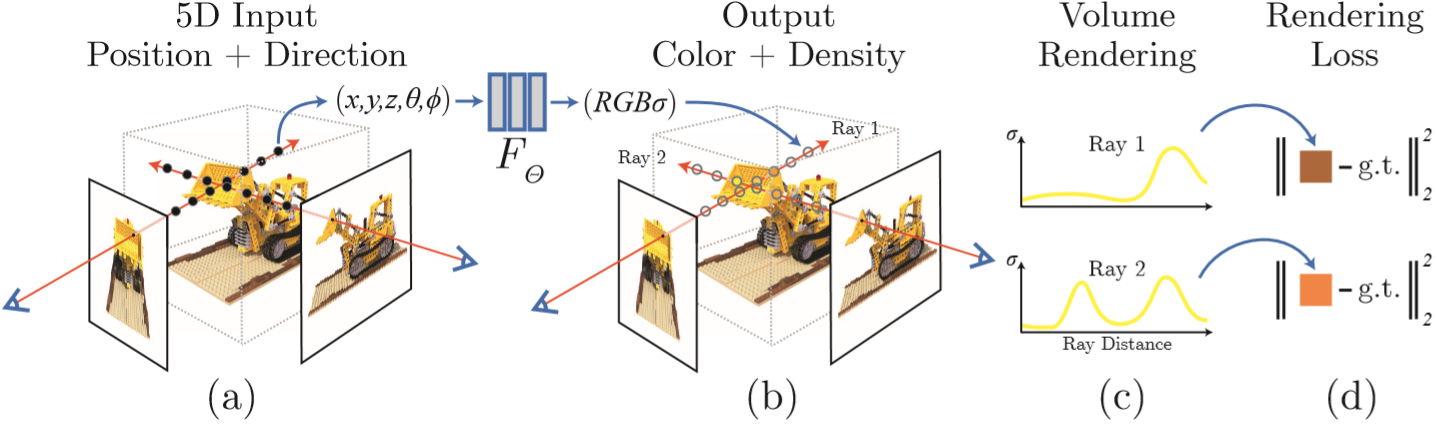
\includegraphics[scale = 1.2]{figures/nerf.png}
    \centering
    \caption{NeRF场景隐式表达与可微渲染过程,图源NeRF\cite{nerf}。沿着相机光线采样5D向量作为输入(a),通过MLP获得密度与颜色(b),最终通过体渲染的方式获得像素最终的颜色(c)。上述过程均可微,因此可以通过最小化观测值与计算值差距进行优化(d)。} \label{nerf}
\end{figure}
\subsection{符号距离场(Signed Distance Function, SDF)}
本文选择使用符号距离场函数\cite{sdf}来对场景的几何信息进行编码,而不使用体密度或占据概率。SDF是一种在空间中隐式表示表面的函数,其数学定义如下:

如果$\Omega$是以$d$为单位的度量空间$X$的子集,那么符号距离场函数$f$定义为:

$$f(x) = \left\{
\begin{aligned}
&d(x,\partial\Omega)&&if\; x\in\Omega \\
-&d(x,\partial\Omega)&&if\; x\notin\Omega\\
\end{aligned}
\right.
$$

$\partial\Omega$指$\Omega$的边界。对任意$x\in X$, $\inf$表示下确界,

$$
d(x,\partial\Omega) := \inf_{y\in \partial\Omega}d(x,y)
$$

简单的说,相较于显示的给定一个点与其法向量以表示一个表面,符号距离场函数映射了空间中一个点到某个表面的最近距离。如图如图\ref{sdf_figure}所示,值的符号取决于该位置位于平面的内部或外部。同时,为限制计算消耗与更精确的表示表面,本文使用带截断值$tr$的TSDF,即绝对值大于此值的SDF值被视为$\pm tr$。
\begin{figure}[htbp]
    \centering
    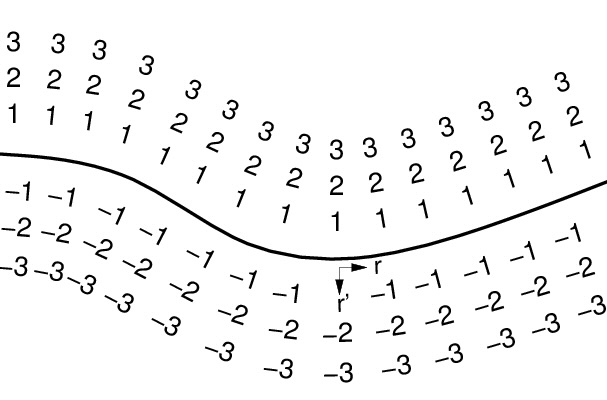
\includegraphics[scale=0.3]{figures/sdf_figure.jpeg}
    \caption{符号距离场函数}\label{sdf_figure}
\end{figure}

符号距离场不需要对几何形状进行离散化或网格化。相反,它可以在连续的空间中定义距离函数。这使得它能够更精确地捕捉到曲线、曲面和体积的几何特征。与此同时,连续的距离函数意味着可以对其进行插值和平滑操作。这使得符号距离场在生成曲线或曲面的过程中能够提供更平滑的结果。进一步,符号距离场可以捕捉到高阶几何特征,例如曲率和法线方向。这些几何信息对于许多应用非常重要,如计算机图形学中的光照和纹理映射。加之其高精度的数据表达与紧密存储特性,相比于传统的体素或网格方法,符号距离场可以更精确的表达几何信息。
\subsection{八叉树(Octree)与空间莫顿码(Morton Code)}
\begin{figure}[htbp]
    \centering
    \subfigure{
    \begin{minipage}[t]{0.47\linewidth}
    \centering
    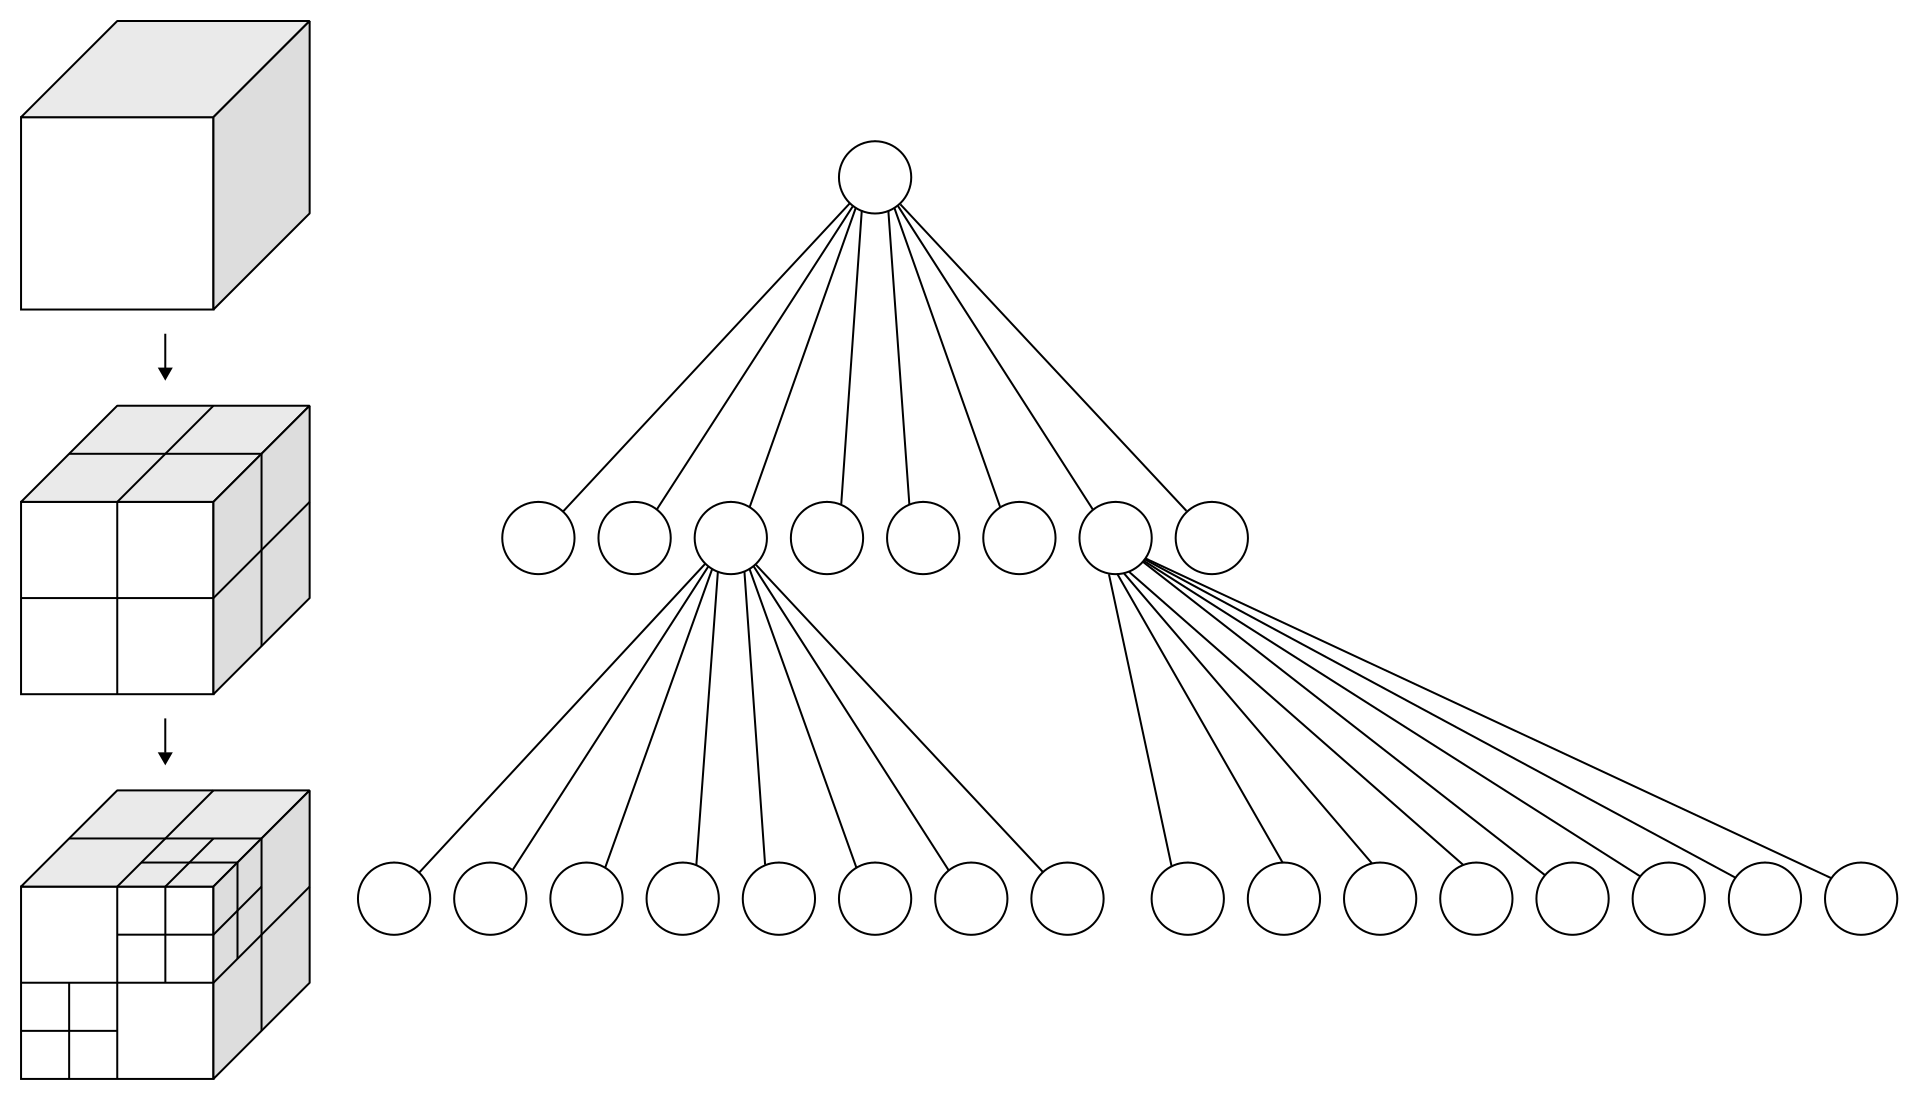
\includegraphics[width=\linewidth]{figures/octree.png}
    \caption{一个三层八叉树示例}\label{octree}
    \end{minipage}
    }
    \centering
    \subfigure{
    \begin{minipage}[t]{0.47\linewidth}
    \centering
    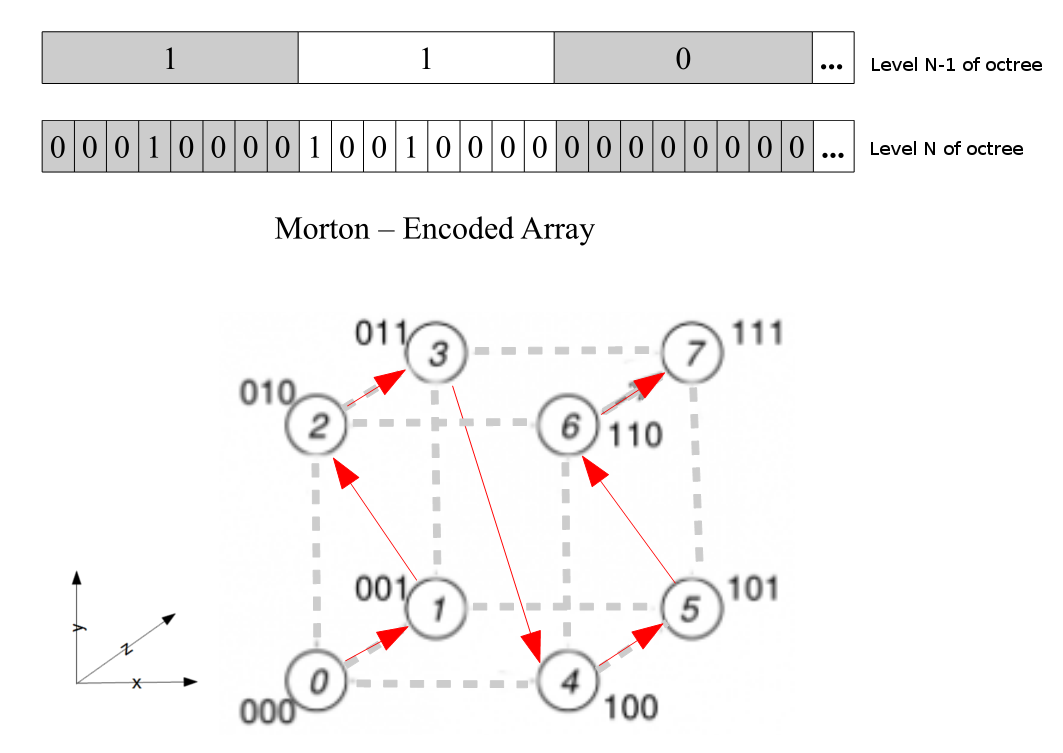
\includegraphics[width=\linewidth]{figures/morton.png}
    \caption{使用莫顿码将空间坐标编码至数组中}\label{morton}
    \end{minipage}
    }
\end{figure}
八叉树是一种用于描述三维空间的树状数据结构。如图\ref{octree},八叉树通过对三维空间的几何实体以循环递归的划分方法进行体元剖分,每个体元具有相同的时间和空间复杂度。在八叉树结构中如果被划分的体元具有相同的属性,则该体元构成一个叶节点;否则继续对该体元剖分成8个子立方体。使用八叉树可以快速进行三维目标的集合运算,如交、并、补、差等,也可快速进行临近点查询和与其他物体的碰撞检测。

为了快速的查询体素八叉树,本文使用了传统的基于体素的SLAM方法\cite{traditionalslam}中的索引方式,将体素坐标编码为莫顿码,并将体素中的信息线性存储,以此达到快速检索的目的。莫顿码是通过将坐标的二进制形式的每个维度的每个比特交叉重组的方式生成的,类似于一种哈希算法,将一个2D或3D坐标转换为一个唯一的索引。如图\ref{morton}所示,给定一个体素的3D坐标$(x,y,z)$,通过遍历其莫顿码,可以快速的找到其在八叉树中的位置。同时,也可以对当前体素的莫顿码进行变换以快速找到其相邻的体素。

\newpage
\section{算法设计}\label{algorithm}
\subsection{系统框架}
本文的系统框架如图\ref{system}所示。该系统以一系列连续的点云帧作为输入,相较于其他使用RGB-D图像作为输入的系统,无需使用相机姿态与内参。该系统维护了两个独立的线程:使用输入数据进行逐帧建图和进行关键帧选择的增量建图线程;在关键帧集合中选择优化对象进行批量训练,以对全局地图进行优化的全局建图线程。

当系统启动时,增量建图线程加载数据,根据每一帧中的点云分配体素和初始化特征。在随后进行的可微渲染过程中,生成采样光线并使用真实数据对地图特征与解码器进行监督训练。在增量线程中使用了一个关键帧选择策略,将符合条件的点云帧放入关键帧集合。全局建图线程维护一个关键帧窗口,对被随机选中的关键帧同步的进行批量采样和渲染,进而对地图进行全局的优化。两个线程共享的数据包括关键帧集合,被嵌入特征的体素网格和解码器参数。
\begin{figure}[htbp]
    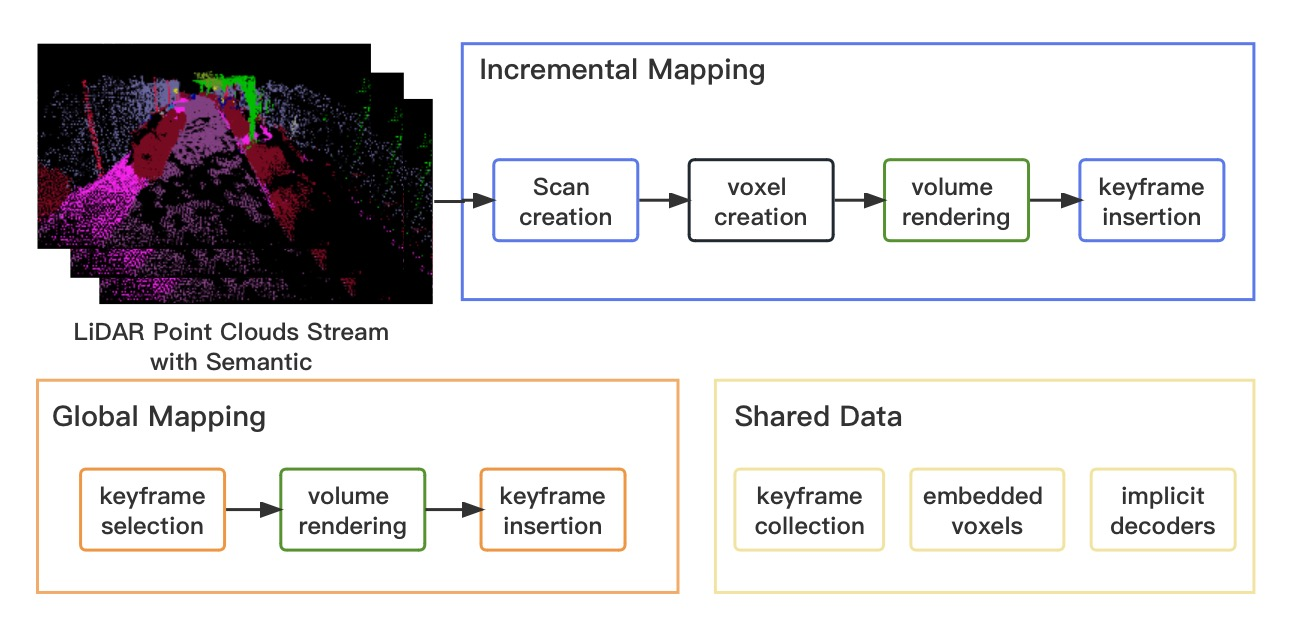
\includegraphics[scale = 0.355]{figures/system.jpg}
    \centering
    \caption{系统概览。该系统维护了两个独立的线程,以带语义的点云作为输入,分别对地图进行增量建图与全局建图。两者共享了包括地图特征在内的资源数据,同步的对地图进行优化。}\label{system}
\end{figure}
\subsection{基于点云的体渲染}
本文使用点云数据进行监督训练,将每一次激光雷达扫描(Scan)的结果作为一帧$f$,因此整个系统输入的数据为一系列连续的点云帧。每一帧包含一个激光雷达3D坐标$\mathbf{x}\in \mathbb{R}^3 $与一个点云集合$P$。其中每一个点云$p\in P$都包含其自身的3D坐标$\mathbf{x}_p\in \mathbb{R}^3$与一个语义标签索引$s\in \mathbb{R}$。
\subsubsection{体素采样}
本文使用一个隐式的SDF解码器$F_\theta$,一个隐式的语义解码器$G_\phi$(其中$\theta$和$\phi$为可优化的网络参数)和一个$N$维的存储在稀疏体素中的特征集合来表示一个场景。这些特征存储在每一个体素的8个顶点上,每一个特征都被相邻的体素共享,这些共享的特征可以优化体素边界上出现的伪影。

由于本文的体素是动态分配的,对于尚未进行建图的区域空间中存在大量的空白体素。因此,在空间中进行分层随机采样的方法会在无效的体素上浪费大量的运算资源。为了提高采样效率,对于当前点云帧中每一个被采样的点云,本文首先通过一个求交运算,检查这条沿着从雷达位置到该点的光线是否穿过了任何有效体素。没有击中任何体素的采样点云会被剔除,因为其不会对渲染产生任何影响。考虑到复杂的大规模场景可能存在较远的边界,本文设置了一个采样点所能影响到的体素的最大数量$M_h$和最大的采样距离$D_{max}$。

如图\ref{shinemapping}所示,对于模拟出的光线,本文将以固定步长在从雷达位置到最大采样距离的有效体素上进行等距采样。对于光线上的任意一个采样点,本文使用其处于的叶子节点上的8个$N$维特征进行三线性插值,得出该点的特征值。随后使用解码器进行解码。
\begin{figure}[htbp]
    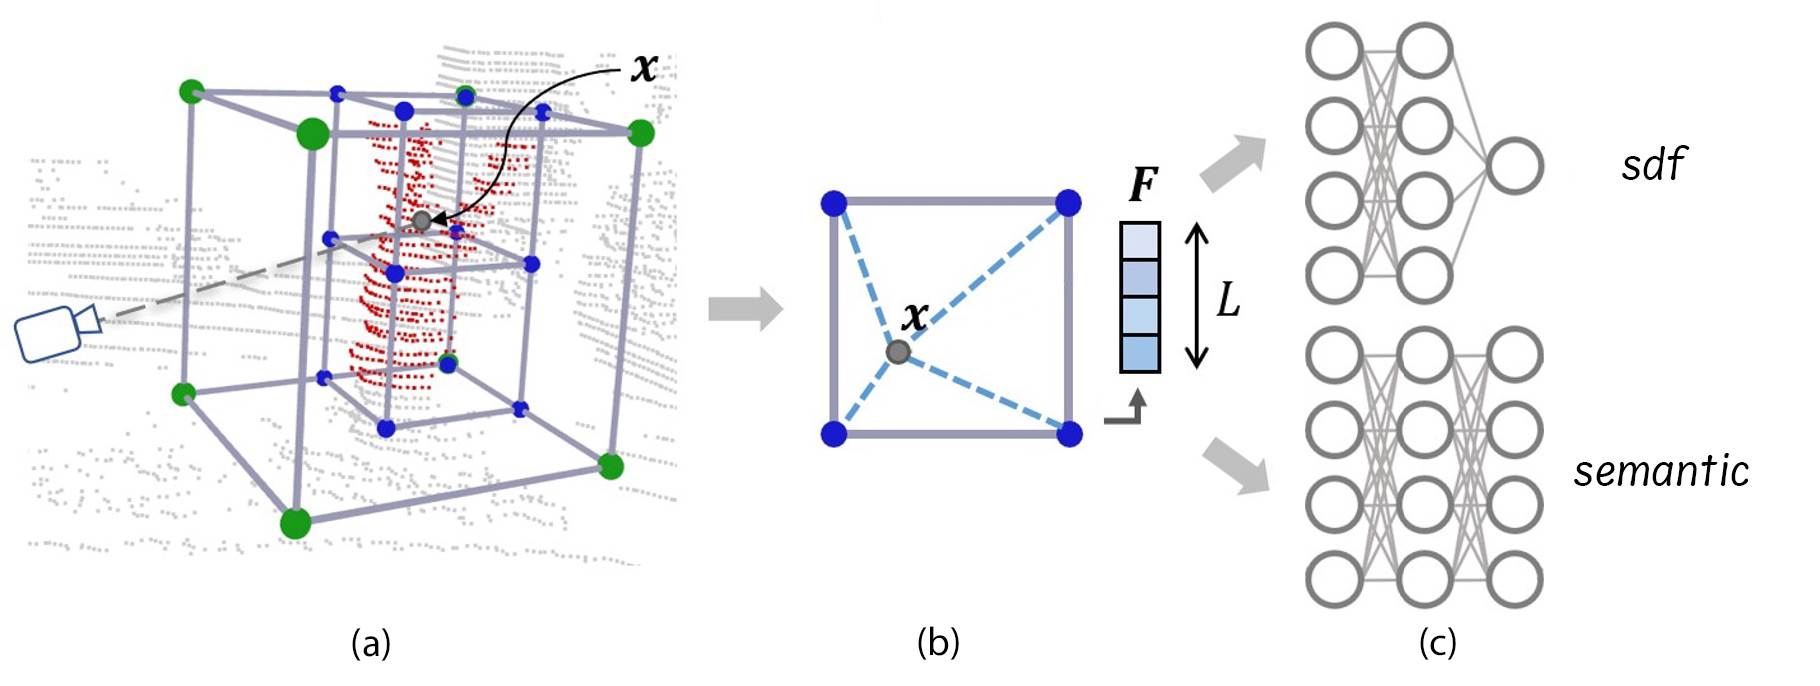
\includegraphics[scale = 0.3]{figures/shinemapping.png}
    \centering
    \caption{一次迭代中的正向传播步骤:首先模拟一条从激光雷达处发出的穿过被采样点云的光线,随后在光线上以固定步长采样(a),对于空间中每一个采样点,对叶子节点体素使用三线性插值计算出特征值(b),最后使用SDF解码器与语义解码器计算出最终结果(c)。}\label{shinemapping}
\end{figure}
\subsubsection{解码器}
如图\ref{shinemapping}所示,本文使用两个较浅的全连接层(MLP)$F_\theta$和$G_\phi$分别用来预测空间中任意一点的SDF值与语义信息。其中$F_\theta$的输出为一个SDF数值,代表该点距离最近表面的距离;$G_\phi$的输出为一个$N_{sem}$维向量,其中$N_{sem}$表示语义标签种类的个数。该向量在推理时会被执行一次argmax函数得到最终语义标签的索引。
\subsubsection{隐式表面渲染}
相较于原始NeRF中使用MLP预测空间中任意一点的体密度,也就是占据概率, SDF能更好的表达几何信息,这也是为什么可以将其用于光线追踪中等任务中,因此本文在训练中直接回归SDF值。下列渲染公式表示了如何从嵌套在体素中的特征中获得该处点云最终的深度$D$和语义向量$\mathbf{S}$。假设在一条光线上采样$N$个点:
\begin{equation}
\begin{alignedat}{2}
    &s_i&&=F_\theta(\mbox{TriLerp}(T_i\mathbf{p}_i,\mathbf{e}))\;,\\
    &\mathbf{S}_i&&=G_\phi(\mbox{TriLerp}(T_i\mathbf{p}_i,\mathbf{e}))\;,\\
    &w_i&&=\mathbf{\sigma}(\frac{s_i}{tr})\cdot\mathbf{\sigma}(-\frac{s_i}{tr})\;,\\
    &\mathbf{S} &&= \frac{1}{\sum_{j=0}^{N-1}w_j}\sum_{i=0}^{N-1}w_i\cdot\mathbf{S}_i\;,\\
    &D &&= \frac{1}{\sum_{j=0}^{N-1}w_j}\sum_{i=0}^{N-1}w_i\cdot d_i
\end{alignedat}
\end{equation}
其中$T_i$表示当前帧激光雷达的位置, $\mathbf{p}_i$表示该点在体素中的相对坐标,$\mbox{TriLerp}(\cdot , \cdot)$表示三线性插值函数, $\mathbf{e}$表示存储在体素中的特征。$F_\theta\mbox{和}G_\phi$分别为带可优化网络参数的解码器。为了计算每一个采样点的权重$w_i$, 本文使用sigmoid函数$\mathbf{\sigma}$计算sdf值$s_i$与先前设置的截断距离$tr$的比值。本文使用该权重对这条光线上的每个采样点的语义向量$\mathbf{S}_i$进行加权积分得到最终结果$\mathbf{S}$。同样的,为了得到深度值,本文对这条光线上每一个采样点的深度进行积分,其中$d_i$为第$i$个采样点的深度。
\subsection{建图}
\subsubsection{地图优化}
为了监督网络训练,本文尝试了多种损失函数,分别为semantic loss, depth loss, free-space loss, SDF loss和二元交叉熵BCE loss。其中semantic loss为多元交叉熵函数,depth loss为L1损失函数。给定采样点云集合$P$:
\begin{equation}
\begin{alignedat}{2}
    &\mathcal{L}_{sem} &&= -\frac{1}{|P|}\sum_{i=0}^{|P|}\sum_{j=0}^{N_{sum}}\mathbf{S}_i^{gt}[j]\log(\mathbf{S}_i[j])\;,\\
    &\mathcal{L}_{depth} &&= \frac{1}{|P|}\sum_{i=0}^{|P|}\| D_i-D_i^{gt}\Vert\;,
\end{alignedat}
\end{equation}
其中$\mathbf{S}_i$和$D_i$为点云帧集合中第$i$个点渲染出的语义向量和深度,与之对应的$\mathbf{S}_i^{gt}$同样为$N_{sem}$维向量,除语义标签索引位置为1之外其余位置均为0, $\mathbf{S}_i[j]$表示其中的第$j$个元素; $D_i^{gt}$为该帧中激光雷达到该点的欧式距离。 

在基于SDF的建图中,需要被关注应该是其SDF值为0的点,因为这些点定义了表面。因此,越接近采样点云的采样点应该对最终SDF值的作用更大,反之,离点云越远的点其作用也更小。本文分别使用了SHINE-Mapping中的二元交叉熵损失函数和Vox-Fusion中的free-space loss和sdf loss两个L2损失函数。

SDF二元交叉熵函数的计算过程为,首先通过带超参数$\sigma$的sigmoid函数$S(x) = 1/(1 + e^{x/\sigma})$,其中超参数$\sigma$用来控制函数的平滑度,将sdf值映射到$[0,1]$区间上。给定一个采样点$\mathbf{x}_i\in \mathbb{R}^3$,计算其投影至表面(假设每个被采样的点云均在表面上)的距离$d_i$,使用经过映射后的值$l_i=S(d_i)$作为监督值。之后应用二元交叉熵作为本文的损失函数:
\begin{equation}
    \mathcal{L}_{bce} = l_i\cdot \log(o_i)+(1-l_i)\cdot\log(1-o_i),\label{bce}
\end{equation}
其中$o_i=S(F_\theta(\mbox{TriLerp}(T_i\mathbf{p}_i,\mathbf{e})))$,即经过映射后的渲染出的SDF值。
free-space loss是为了使解码器学习截断距离$tr$,尤其是位于采样点表面附近的符号为正的截断区域内的截断值,然后使用sdf loss在截断区域内学习SDF值以此来使解码器精确的表示表面。本文在渲染时将SDF值为$-tr$的点剔除。
\begin{equation}
    \begin{alignedat}{2}
        &\mathcal{L}_{fs} &&= \frac{1}{|P|}\sum_{p\in P}\frac{1}{S_p^{fs}}\sum_{s\in S_p^{fs}}(D_s-tr)^2,\\
    &\mathcal{L}_{sdf} &&= \frac{1}{|P|}\sum_{p\in P}\frac{1}{S_p^{tr}}\sum_{s\in S_p^{tr}}(D_s-D_s^{gt})^2.\label{voxloss}
    \end{alignedat}
\end{equation}
本文在优化时对地图特征与解码器均应用了ADAM\cite{adam}优化方法,最终的损失函数为:
\begin{equation}
    \mathcal{L} = \lambda_{sem}\mathcal{L}_{sem}+\lambda_{depth}\mathcal{L}_{depth}+\lambda_{bce}\mathcal{L}_{bce}+\lambda_{fs}\mathcal{L}_{fs}+\lambda_{sdf}\mathcal{L}_{sdf}
\end{equation}
其中$\lambda$表示不同损失函数的权重。在实际情况中,对于SDF的监督通常只使用式\ref{bce}或式\ref{voxloss}中的一种损失函数。
\subsubsection{动态体素管理}
相较于在运行前就将整个场景编码,本文只关注已经被观察到的场景表面,因此使用动态体素管理方法进行体素的分配与搜索。本文将整个场景使用八叉树进行切分为互不包含的体素。这些体素与坐标轴平行,作为组成场景的元素和八叉树的叶子节点。

首先将尚未观察到的场景区域的叶子节点初始化为空,当新的一帧进入系统时,将该帧中的所有点云变化至世界坐标系。如果这些点云落在了尚未分配的体素中,系统将为这些点云分配新的体素。由于本文设置了八叉树的最大层树$L_{max}$,因此每个点云会被放置在最小的叶子节点中。该过程不需要采样,而是对所有点进行计算,因此使用八叉树结构可以更快的进行分配和索引。
\subsubsection{全局建图与关键帧选择}\label{forgettingsection}
\begin{figure}[htbp]
    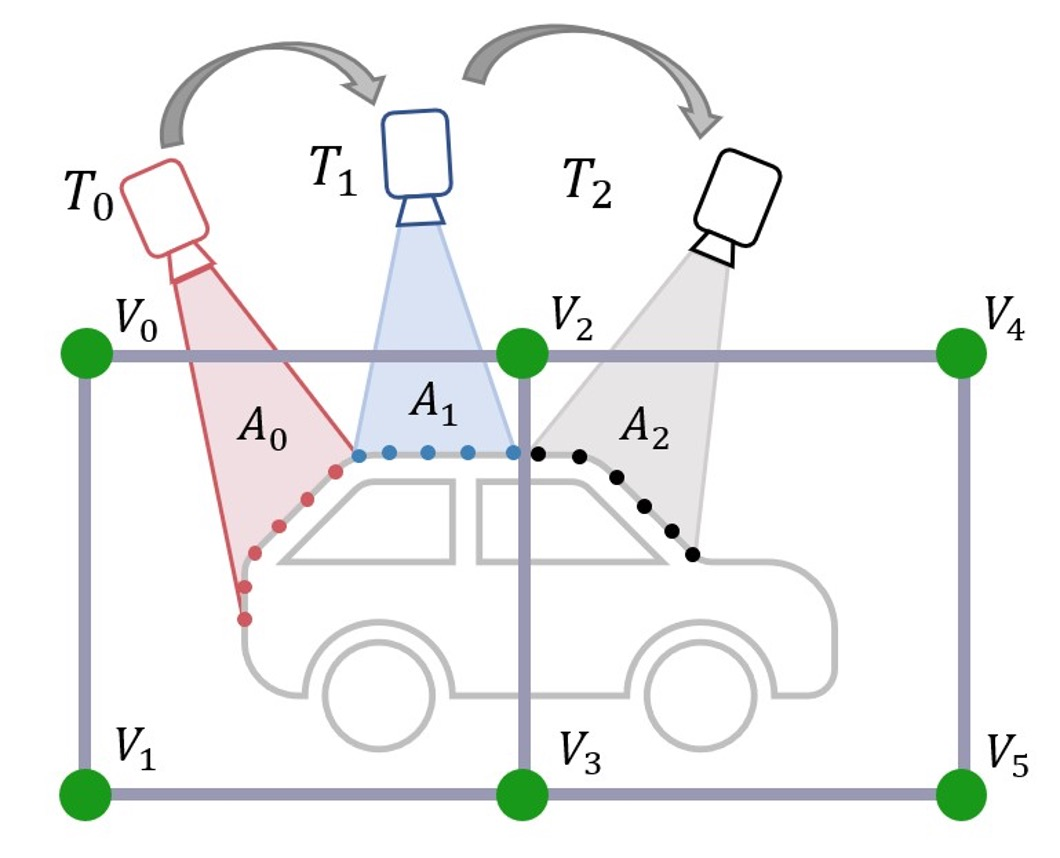
\includegraphics[scale = 0.2]{figures/forgetting.jpg}
    \centering
    \caption{在特征网格中进行增量建图时发生遗忘问题的例子,图源SHINE-Mapping\cite{shine}} \label{forgetting}
\end{figure}
将大规模场景以增量建图方法编码会受到灾难性遗忘(Catastrophic Forgetting)问题的限制。如图\ref{forgetting}所示,在每一帧中($T_0, T_1$和$T_2$),系统仅能观察到环境的部分信息。在增量建图中的第$T_0$帧,使用从区域A0获取到的信息优化存储在网格中的特征$V_0, V_1, V_2$和$V_3$,因此$V_0, V_1, V_2$和$V_3$这4个特征将能较精确的表示区域A0的几何信息。然而当相机向前移动,使用T1帧更新$V_0, V_1, V_2$和$V_3$的特征时,网络将仅关注生成$A_1$时的损失,不再关注$A_0$区域的表现。当相机进一步移动至$T_2$帧时,$V_2$和$V_3$中的特征将再次被更新,但网络无法保证不会影响到$A_0$和$A_1$区域的建图精度。这就是遗忘问题发生的原因。

为了解决灾难性遗忘问题,本文记录关键帧对网络进行重复训练。系统维护了一个关键帧集合K,使用Vox-Fusion中的策略,即八叉树体素结构的变化量决定何时插入关键帧:每当新的一帧出现时,体素管理系统会执行求交运算得出需要新分配体素的数量$N_c$,而当前存储的体素数量为$N_o$,当两者比值$p_{kf}=N_c/N_o$大于某一阈值时,当前帧将被插入关键帧集合。某种极端情况下,当相机移动处于一个循环状态时,可能出现只有极少体素或没有体素被新分配,导致永远没有关键帧被插入。因此,本文也设定了相邻关键帧的最大距离,例如,当之前的$N$帧都不是关键帧时,自动插入一个关键帧。

在第全局建图线程中,本文使用一个大小为$N_{kf}$的窗口从关键帧集合$K$中随机选取$N_{kf}$个关键帧,与当前帧一起,共$N_{kf}+1$帧作为优化目标对地图进行全局优化,与增量建图线程同步进行。在增量建图结束后,使用全局建图线程随机选择优化目标对整个地图执行$N_f$次迭代训练,完成最后的建图优化。

\newpage
\section{系统实现}\label{implement}
\subsection{增量建图与全局建图线程}
本文使用Python与C++实现该算法。八叉树相关实现,如分配,索引,求交运算,采样等使用C++完成。 Python中主要实现了IncrementalMapping与GlobalMapping两个类。为实现两个线程共享数据,本文使用Python多线程管理工具multiprocessing.managers进行通讯,将地图体素,地图特征,关键帧集合与解码器及其参数共享,使得两个线程能够对上述数据进行同步更新。两个主要线程算法的伪代码如算法\ref{incrementalmapping}和算法\ref{globalmapping}所示。在具体的实现过程中,本文构造了一个用于激光雷达数据的转换器,将激光雷达数据转换为附带语义标签的点云数据,以此读入不同格式的激光雷达数据集。

为了保证增量建图线程与全局建图线程在获取与修改共享资源,即体素网格,地图特征,解码器参数时,不发生资源竞争导致错误,本文使用了锁对上述资源进行管理。当进程访问和修改上锁的资源时会发生阻塞,等待其他线程操作结束后释放锁。除此之外,在训练结束后,本文实现了对模型进行采样推理并提取网格地图,并使用相关算法对结果进行精度评估,该部分将在\ref{metric}节详细介绍。
\begin{algorithm}
    \caption{增量建图}\label{incrementalmapping}
    \begin{algorithmic}[1]
      \Require
        包含位姿和语义信息的点云帧集合$S_{frame}$
      \Ensure
        体素集合$S_{voxel}$;
        地图特征集合$S_{feature}$;
        解码器网络参数$\theta, \phi$;
        关键帧集合$S_{keyframe}$
      \Function{IncrementalMapping}{$S_{frame}$}
      \For{each $frame\in S_{frame}$}
      \State $S_{voxel}\gets S_{voxel}+$ \Call{CreateVoxel}{$frame$}
      \State $S'_{feature}, \theta', \phi'\gets$\Call{Mapping}{$frame$}
      \State $S_{feature},\theta,\phi\gets$\Call{UpdateSharedData}{$S'_{feature}, \theta', \phi'$}
      \If{\Call{IsKeyFrame}{$frame$}}
      \State $S_{keyframe}\gets S_{keyframe}+frame$
      \EndIf
      \EndFor
      \State \Return{$S_{voxel},S_{feature},\theta,\phi,S_{keyframe}$}
      \EndFunction

      \Function{Mapping}{$frame$}
      \State $rays \gets$\Call{SampleRays}{$frame$}
      \For{each $ray\in rays$}
      \If{\Call{IsIntersect}{$ray,S_{voxel}$}}
      \State $points\gets$\Call{SamplePoints}{$ray$}
      \State \Call{Render}{$points,S_{feature},\theta,\phi$}
      \State $S'_{feature}, \theta', \phi'\gets$\Call{Optimize}{$S_{feature}, \theta, \phi$}
      \EndIf
      \EndFor
      \State \Return{$S'_{feature}, \theta', \phi'$}
      \EndFunction
    \end{algorithmic}
\end{algorithm}

\begin{algorithm}
    \caption{全局建图}\label{globalmapping}
    \begin{algorithmic}[1]
      \Require
        关键帧集合$S_{keyframe}$
      \Ensure
        体素集合$S_{voxel}$;
        地图特征集合$S_{feature}$;
        解码器网络参数$\theta, \phi$
        
      \Function{GlobalMapping}{$S_{keyframe}$}
      \State$optimizeTargets\gets$\Call{RandomSelectFrames}{$S_{keyframe}$}
      \State $S'_{feature}, \theta', \phi'\gets$\Call{Mapping}{$optimizeTargets$}
      \State $S_{feature},\theta,\phi\gets$\Call{UpdateSharedData}{$S'_{feature}, \theta', \phi'$}
      \State \Return{$S_{voxel},S_{feature},\theta,\phi,S_{keyframe}$}
      \EndFunction
    \end{algorithmic}
\end{algorithm}

\subsection{采样与渲染流程}
\begin{figure}[htbp]
    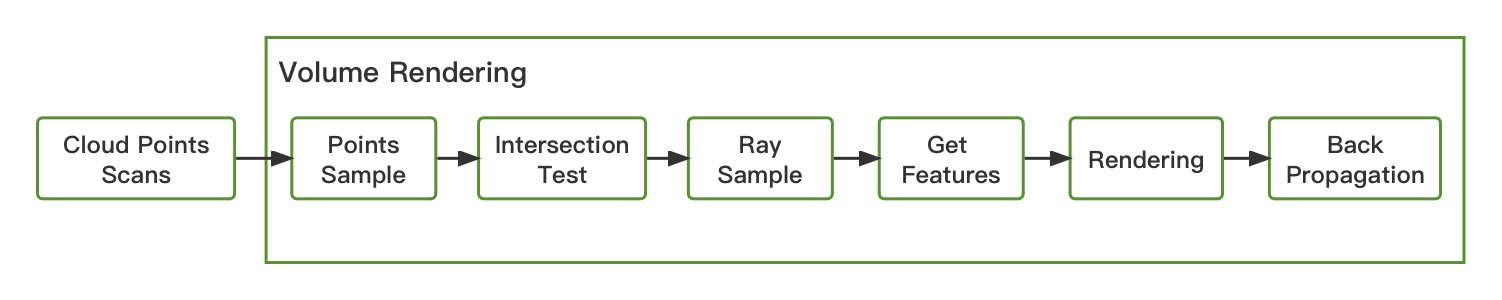
\includegraphics[scale = 0.31]{figures/renderpipeline.jpg}
    \centering
    \caption{采样与渲染流水线。}\label{renderpipeline}
\end{figure}
为了加快系统运行速度,除去算法在无效空间内的运算,本文针对体素分配的策略,对与渲染相关的无效采样点进行了剔除。如图\ref{renderpipeline}所示,首先对一次扫描的结果进行采样,随机选择作为优化目标帧中的点构造光线。为除去对渲染结果无影响的点,对每一条光线进行与已分配体素的求交运算。该求交运算将返回每条光线所碰撞体素的索引与数量,碰撞数量为0的光线将被剔除。

根据在上一步得到的体素索引中,对每条光线进行等距采样,得到一系列采样点的空间坐标。系统将根据体素索引获取特征值索引。通过得到已分配体素的特征值进行三线性插值,进入解码器进行特征提取。最终计算损失函数后进行反向传播优化地图与解码器。
\clearpage
\section{实验}\label{numerical experiments}
\subsection{地图提取}
本文使用训练完毕的地图特征与解码器进行推理并导出地图的顶点与面元数据,以网格格式对结果进行评估。对于网格中每一个被分配的体素,本文将其再次细分为$N \times N \times N$个部分,直接推理出其内部$N^3$个点的SDF值和语义信息。如图\ref{marching}所示最终使用marching cubes\cite{marchingcubes}等值面提取算法提取出地图的所有顶点与表面,并将语义信息映射为顶点颜色。
\begin{figure}[htbp]
    \centering
    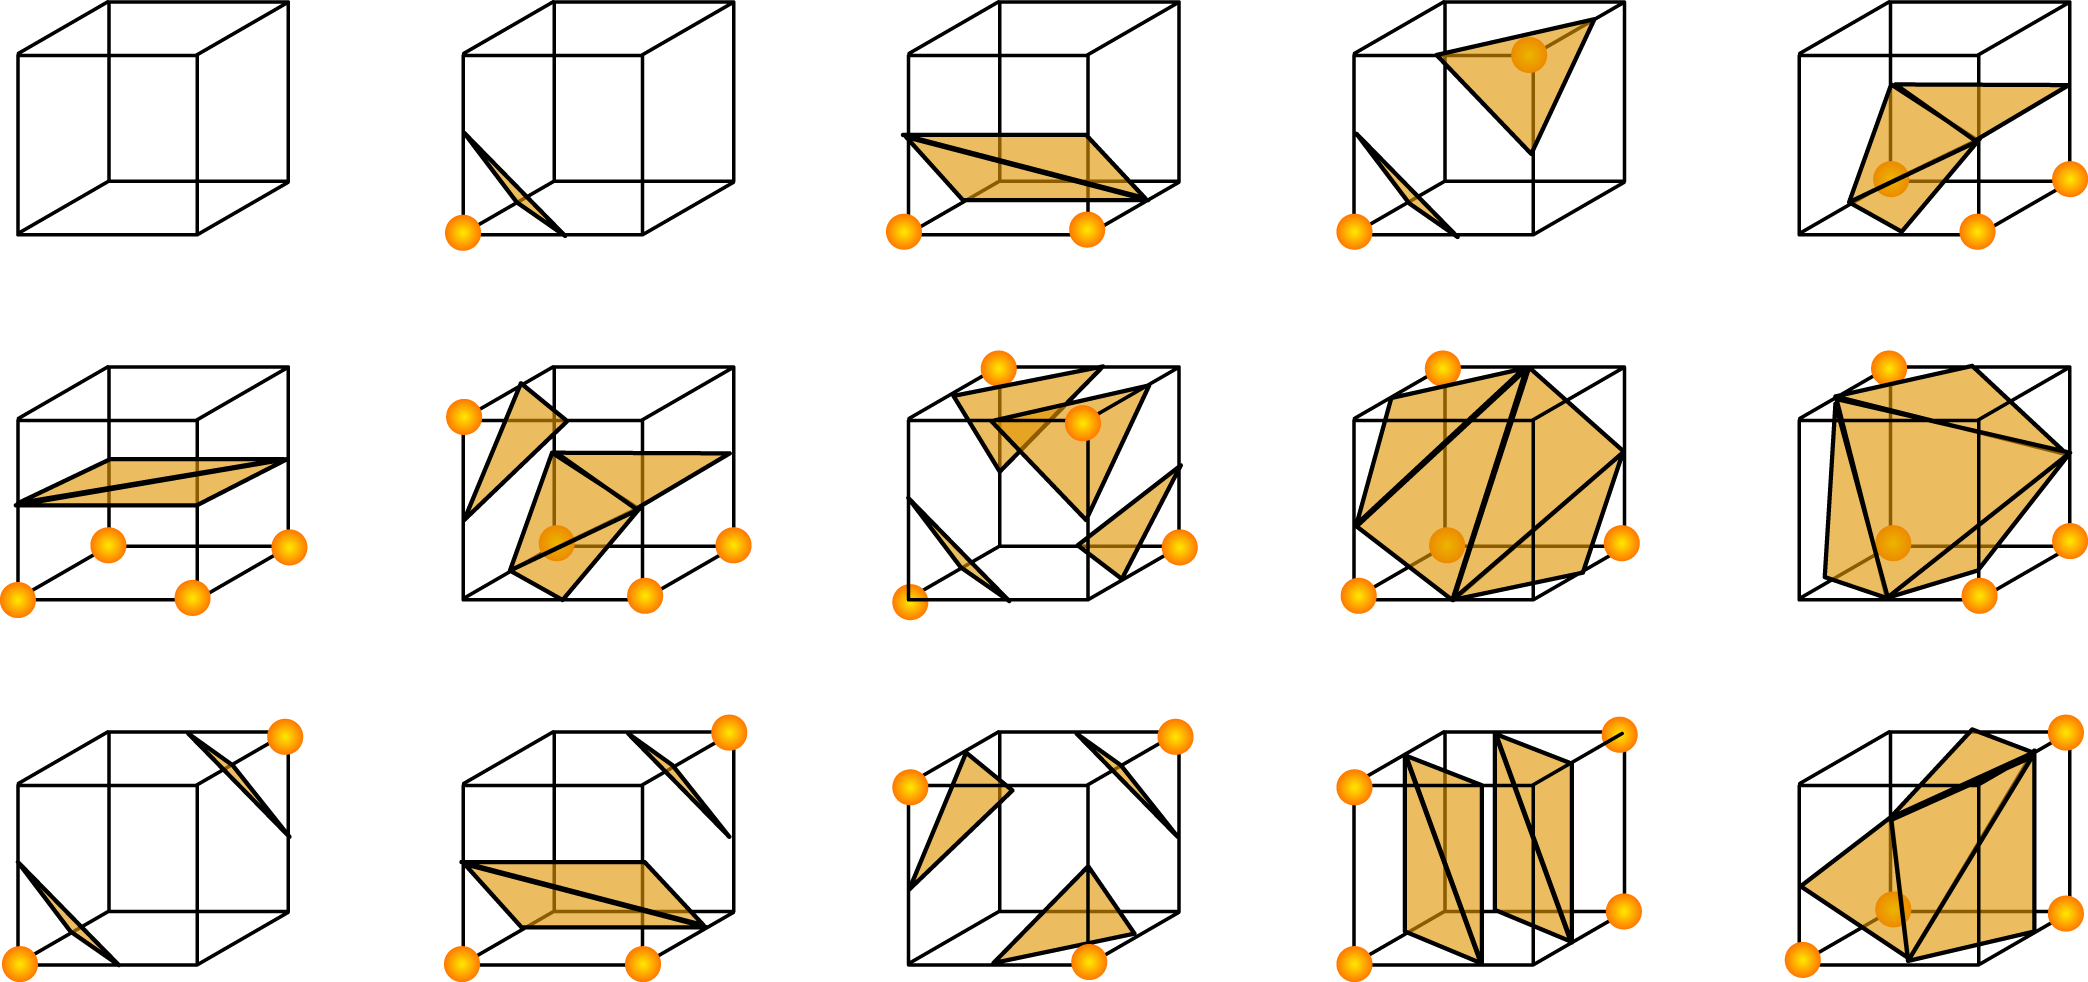
\includegraphics[scale=0.7]{figures/MarchingCubes.png}
    \caption{marching cube算法\cite{marchingpicture}。首先将空间划分为立方体网格,根据顶点处数值与等值面的关系将立方体分为14种状态。最后根据等值面穿过边的状态生成相应的三角片元。}\label{marching}
\end{figure}
\subsection{评价指标}\label{metric}
为评价重建地图的几何精度,本文使用KD树\cite{kd}(K-Dimension Tree)和KNN\cite{knn}(K-Nearest Neighbors)算法分别从两组顶点数据中计算最邻近点的距离,并使用以下5个指标对重建结果进行评价:距离误差,准确率,召回率, L1倒角距离(Chamfer-L1)和F1-score。进一步,本文将距离误差称为完成度(Completeness),将召回率称为完成率(Completeness Ratio)。

完成度指的是Ground Truth中每个点与其预测结果中的对应点的平均距离。Chamfer-L1距离,也称为曼哈顿倒角距离或L1倒角距离,用于衡量两个集合之间的最短距离。其计算方式是取目标形状的每个边缘点或曲线上的点与参考形状的边缘点或曲线上的点曼哈顿距离后计算平均值或求和。本文设置了一个阈值$threshold$以表示两个点是否重合,若两点距离$d<threshold$,则表示两者重合,即重建成功。使用该方法得出重建结果的准确率与召回率。

具体地说,对于Ground Truth顶点集合与由本文方法重建出的顶点,分别对其进行下采样得到顶点集合$V_{gt}$和$V_{pred}$。接下来对$V_{gt}$中的每一个顶点执行KNN算法,找到其到$V_{pred}$中最近点的距离,得到一个距离集合$D_{r}$。同样的,对$V_{pred}$中的每一个点找到其在$V_{gt}$中距离最近的点,将其距离记录为$D_{p}$。上述各项指标的计算公式如下所示:
\begin{equation*}
\begin{alignedat}{2}
D'_{p} &= \{d \in D_{p} \mid d < threshold\}\;,\\
D'_{r} &= \{d \in D_r\mid d<threshold\}\;,\\
Completeness &= \frac{1}{|D_{r}|}\sum_{i=0}^{|D_{r}|}D_{r}[i]\;\\
Accuracy&= \frac{1}{|D'_{p}|}\sum_{i=0}^{|D'_{p}|}D'_{p}[i]\;,\\
Recall &=\frac{1}{|D'_{r}|}\sum_{i=0}^{|D'_{r}|}D'_{r}[i]\;,\\
Chamfer\_L1 &= \frac{1}{2}\left(Completeness + \frac{1}{|D_{p}|}\sum_{i=0}^{|D_{p}|}D_{p}[i]\right)\;,\\
F1\_score &= \frac{2\times Accuracy\times Recall}{Accuracy + Recall}
\end{alignedat}
\end{equation*}

为评估重建语义建图的精度,本文在数据集点云中进行采样,使用采样点的坐标在完成建图的模型中进行推理得到采样点语义。随后将其与采样点数据集的label进行比较计算得到。本文使用的指标为准确率和交并比,其计算公式为:
\begin{equation*}
    \begin{alignedat}{2}
    \mbox{AUC} &=\quad\;\frac{TP}{TP+FP}\\
    \mbox{IoU} &=\frac{TP}{TP + FP + FN}
    \end{alignedat}
\end{equation*}
\subsection{实验设置}
\subsubsection{数据集}
本文的方法在3个公开的户外激光雷达数据集上进行了定性和定量的测试:(1)人工合成的MaiCity数据集\cite{maicity},模拟使用64线无噪声激光雷达对城市场景扫描序列组成。(2)真实世界的Newer College数据集\cite{ncd},该数据集在牛津大学内使用手持激光雷达记录,具有厘米级测量噪声和大量运动失真。其地面数据使用地面扫描仪获得。两者均带有地面附近的Ground Truth网格数据用作评估。(3) KITTI\cite{KITTI}是目前最大的无人驾驶场景下的计算机视觉算法评测数据集, SemanticKITTI\cite{SemanticKITTI}为其点云数据标注了语义信息。其数据包括激光雷达与RGB-D数据流等,每一帧中出现多个车辆或行人,包含超过20种语义标签类型。
\subsubsection{参数选择}
本文中的两个解码器均为两层全连接层,其中SDF解码器每层有128个节点,语义解码器有256个节点。对于每一帧数据采样1024个点进行训练,设定关键帧窗口大小为5。对于不同的数据集,本文使用表\ref{parameters}中设定的超参数进行训练:
\begin{table}[htbp]
    \centering
    \caption{对于不同数据集,本文方法设定的参数列表}\label{parameters}
    \begin{tabular}[htbp]{llcccc}
        \toprule
        \multicolumn{2}{l}{数据集} & 体素大小(m) & 采样间距(m) & 截断距离(m) &最大碰撞体素数 \\
        \midrule
        \multicolumn{2}{l}{KITTI} & 0.4 & 0.2 &0.3 &20\\
        \multicolumn{2}{l}{Mai City} & 0.2 &0.1&0.2&10\\
        \multicolumn{2}{l}{New College} & 0.4 &0.2&0.3&20\\
        \bottomrule
    \end{tabular}
\end{table}
\subsection{实验设计}

无人驾驶仿真系统需要高精度的地图,包括道路与车辆的几何信息等。这些环境信息将提供给无人驾驶系统以帮助其做出准确的决策并进行评估。语义信息可以使无人驾驶系统更好的理解环境。因此准确的语义信息可以在无人驾驶系统进行语义分割与预测任务时作为监督信息与评估指标。在无人驾驶系统使用地图进行仿真时,实时的模型推理是必需的。最后,准备数据集,即在为无人驾驶系统创建大规模室外真实地图以验证其算法时,需要可接受的时间成本。针对以上需求,本文设置了以下定性与定量实验以验证\ref{algorithm}章中提出的优化算法的有效性。同时证明在建图精细度与时间空间代价上,相较于传统建图算法与其他神经隐式表达建图算法,本文在不同场景下具有优势:
\begin{itemize}
	\item 是否使用关键帧选择策略进行全局建图,以证明该优化算法克服遗忘问题的有效性。
	\item 使用式\ref{bce}或式\ref{voxloss}中的损失函数监督SDF训练的对比实验,以证明使用二元交叉熵可以更好的使网络学习场景表面。
	\item 使用不同方法在合成场景与真实世界场景的数据集中与本文方法进行定性的测量与比较,以证明本文方法在几何与语义建图精度的各项指标中具有优势。
	\item 测量系统关键步骤进行的耗时与评估系统性能,证明本文加速优化算法的有效性与对整体性能的提升;计算不同方法的内存消耗以证明本文在相同分辨率与精细度下使用较低的内存。
\end{itemize}
\subsection{实验结果}
本文进行了是否使用关键帧进行全局建图的对比实验。如图\ref{replay}所示,在左图中只使用增量建图线程对KITTI数据集00序列进行建图。地图重建的精细度与准确度随着当前帧位置而变化,即当前帧与当前帧紧邻的帧所影响到的部分场景效果较好。在增量建图线程运行至50帧时,地图右侧新观察到的部分建图效果较好,左侧首先建图的部分已经出现了遗忘问题,地图特征出现缺失,不再连续。当建图线程运行至100帧时,可以看到地图左侧大部分区域的地图细节已经被遗忘,只能解码出大致的轮廓,仅仅只有地图右侧正在建图的区域有较好的建图效果。

当使用\ref{forgettingsection}节描述的关键帧选择策略与开启全局建图线程后,如右图所示,即使激光雷达移动至100帧所在位置时,场景中所有已被观察部分的地图特征均被完整保留,遗忘问题得到了明显改善。实验证明通过这种方法可以降低神经网络的遗忘问题对增量建图的影响。
\begin{figure}[p]
	\centering
	\begin{minipage}{0.5\linewidth}
		\centering
		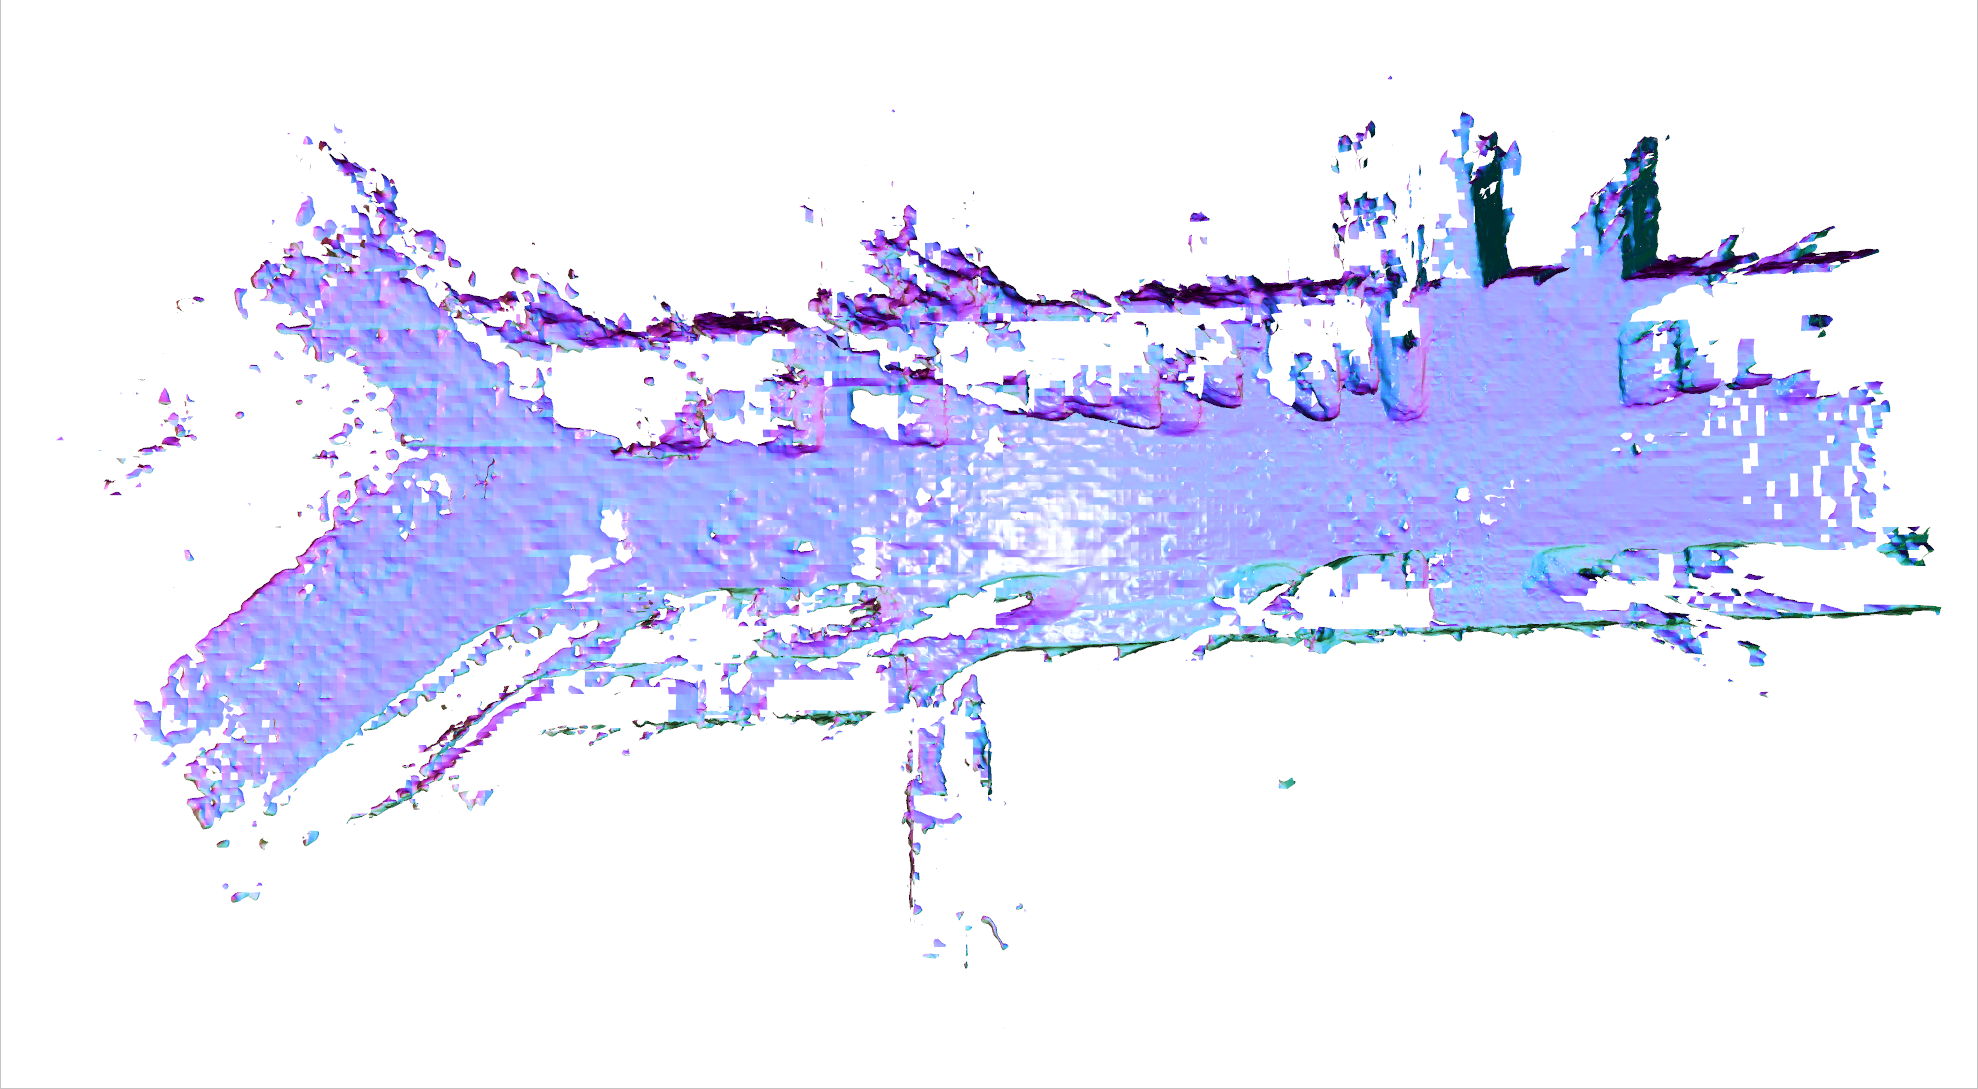
\includegraphics[width=1\linewidth]{figures/50w.png}
        \caption*{不使用replay策略训练50帧}
	\end{minipage}\hfill
	\begin{minipage}{0.5\linewidth}
		\centering
		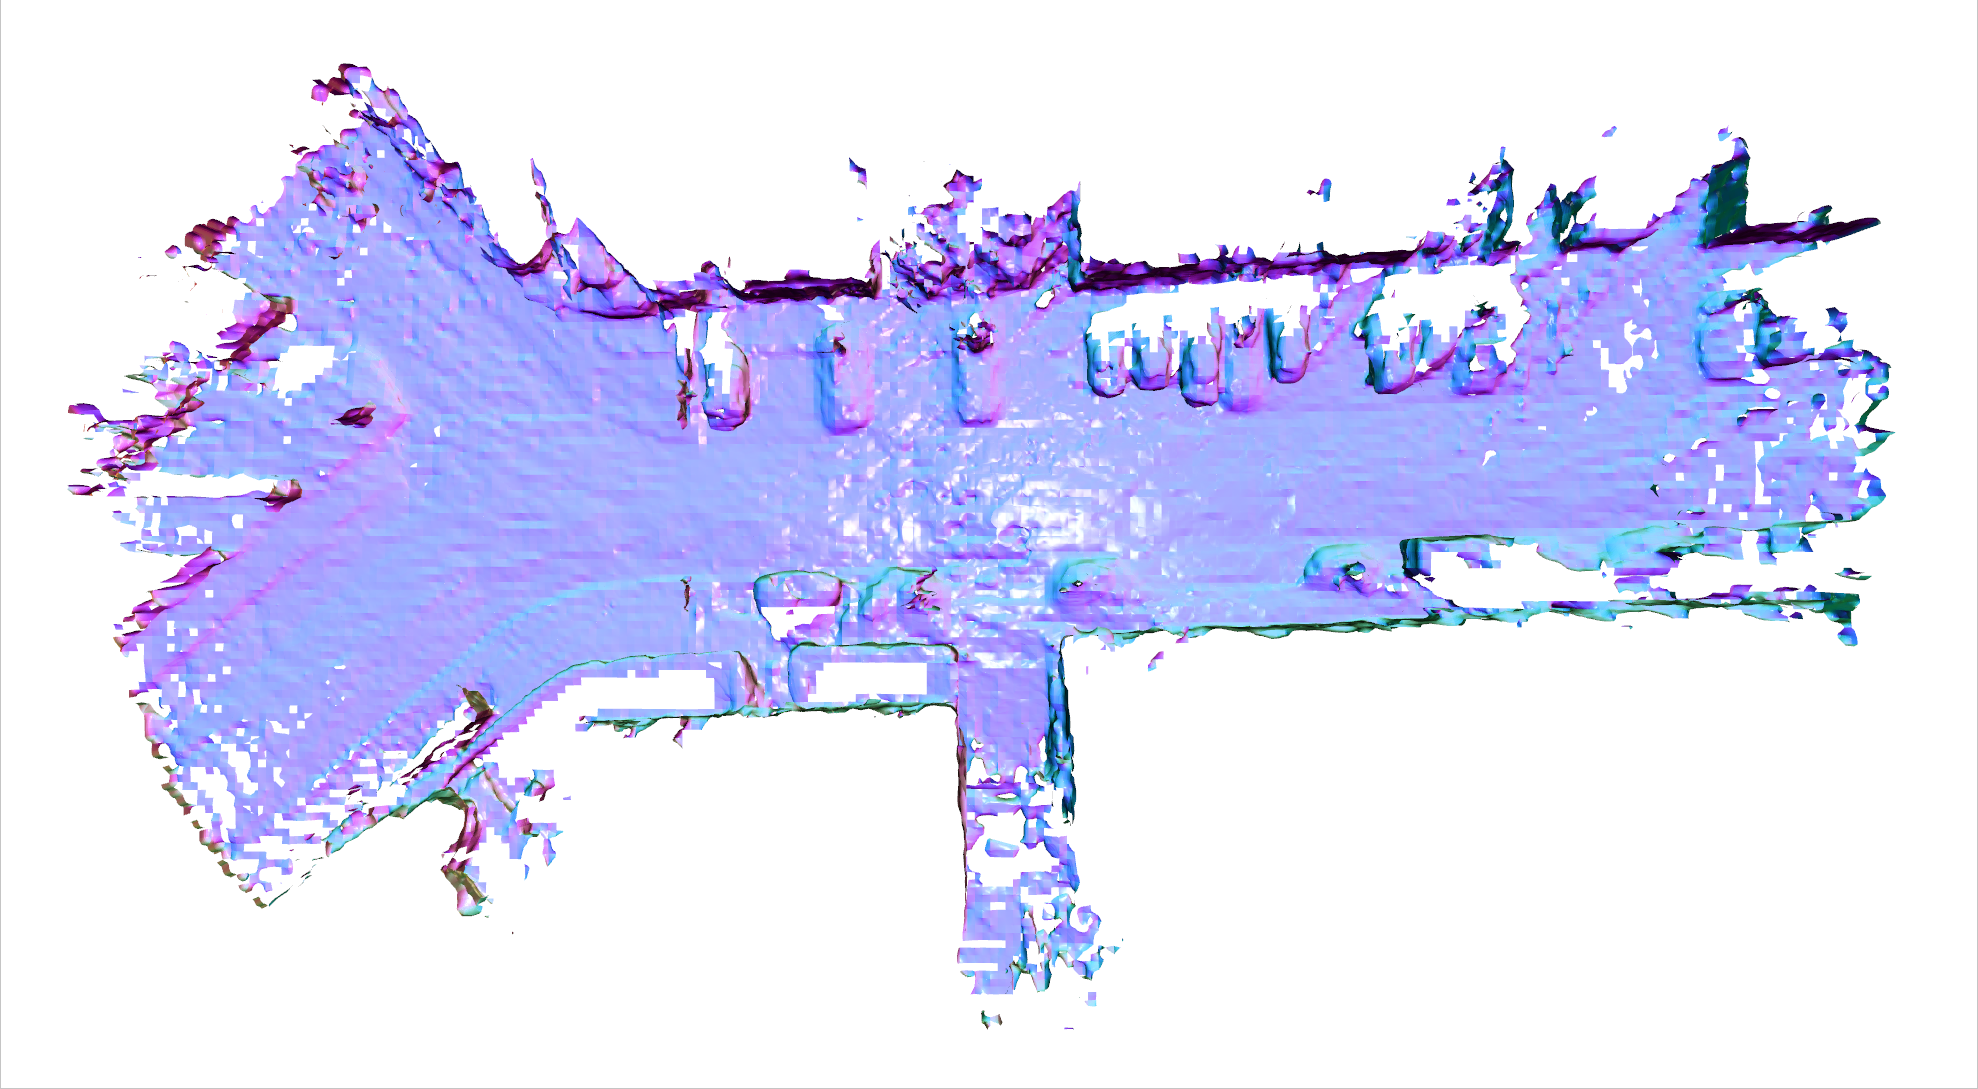
\includegraphics[width=1\linewidth]{figures/50o.png}
        \caption*{使用replay策略训练50帧}
	\end{minipage}
    \vfill
	\begin{minipage}{0.5\linewidth}
		\centering
		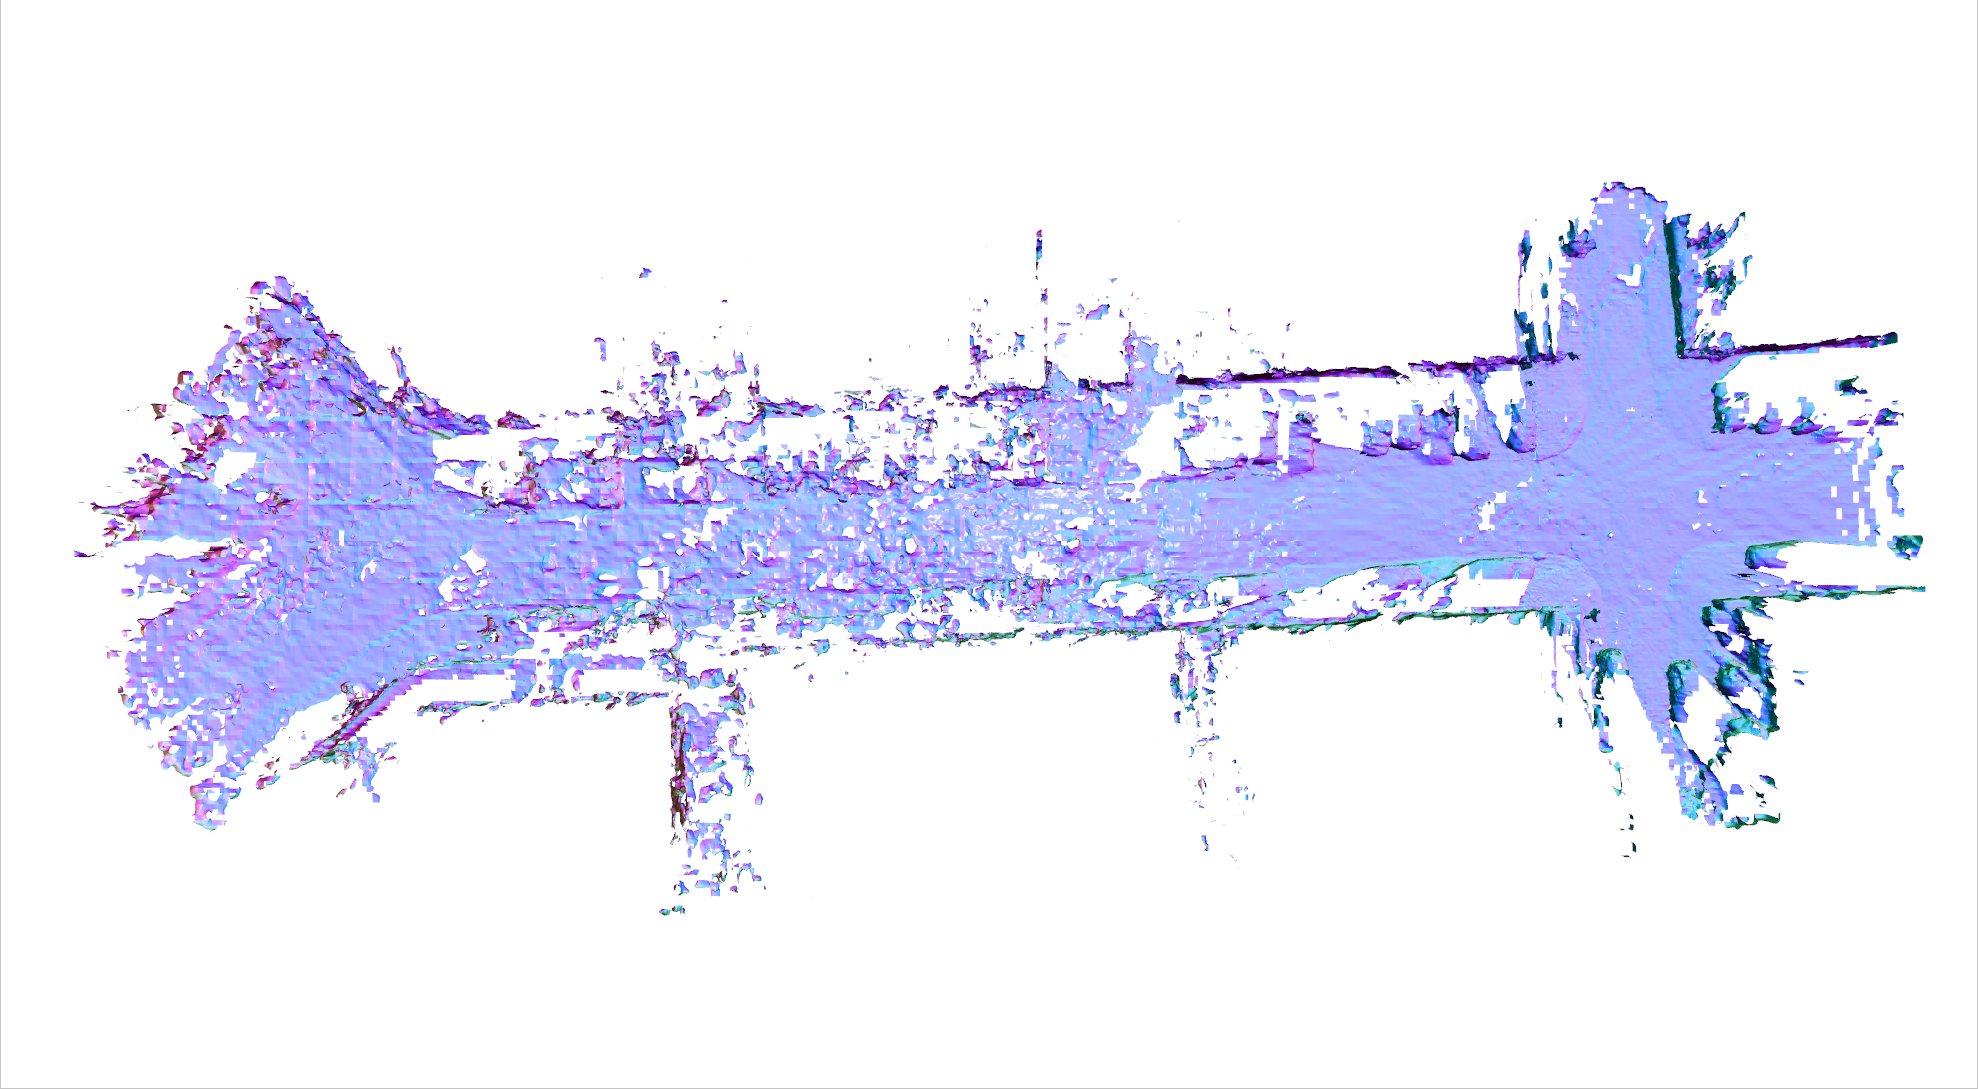
\includegraphics[width=1\linewidth]{figures/100w.png}
        \caption*{不使用replay策略训练100帧}
	\end{minipage}\hfill
	\begin{minipage}{0.5\linewidth}
		\centering
		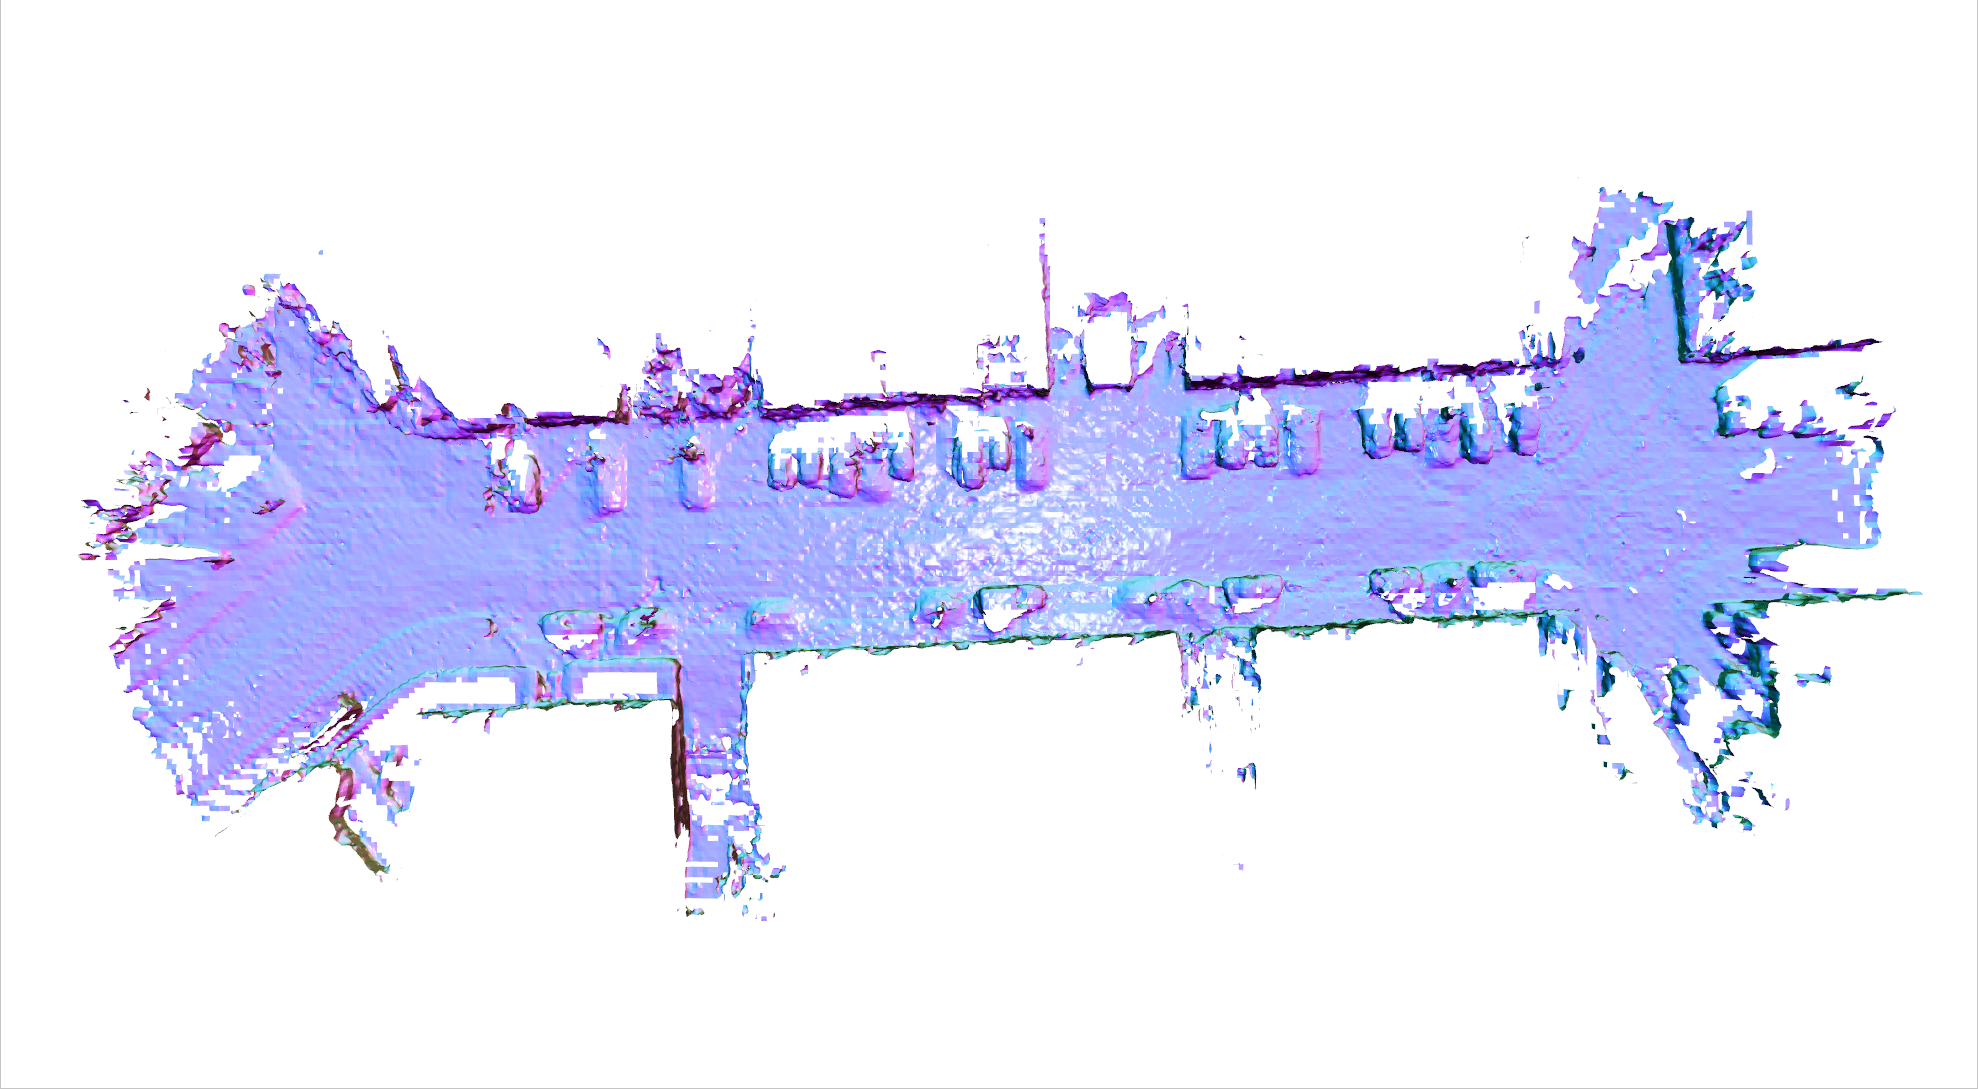
\includegraphics[width=1\linewidth]{figures/100o.png}
        \caption*{使用replay策略训练100帧}
	\end{minipage}
    \caption{在KITTI数据集上是否使用关键帧replay策略的对比实验。在没有使用全局建图线程选择关键帧进行建图的情况下,即使激光雷达只前进50帧时,之前训练的地图部分也会出现遗忘问题。当激光雷达前进100帧时,前50帧所内存的地图信息已经变得非常稀疏。右图使用关键帧选择与全局建图方法后,遗忘问题得到了明显改善,先前的建图准确度与当前帧所在位置无显著联系。}\label{replay}
\end{figure}

\begin{figure}[htbp]
	\centering
	\begin{minipage}{0.45\linewidth}
		\centering
		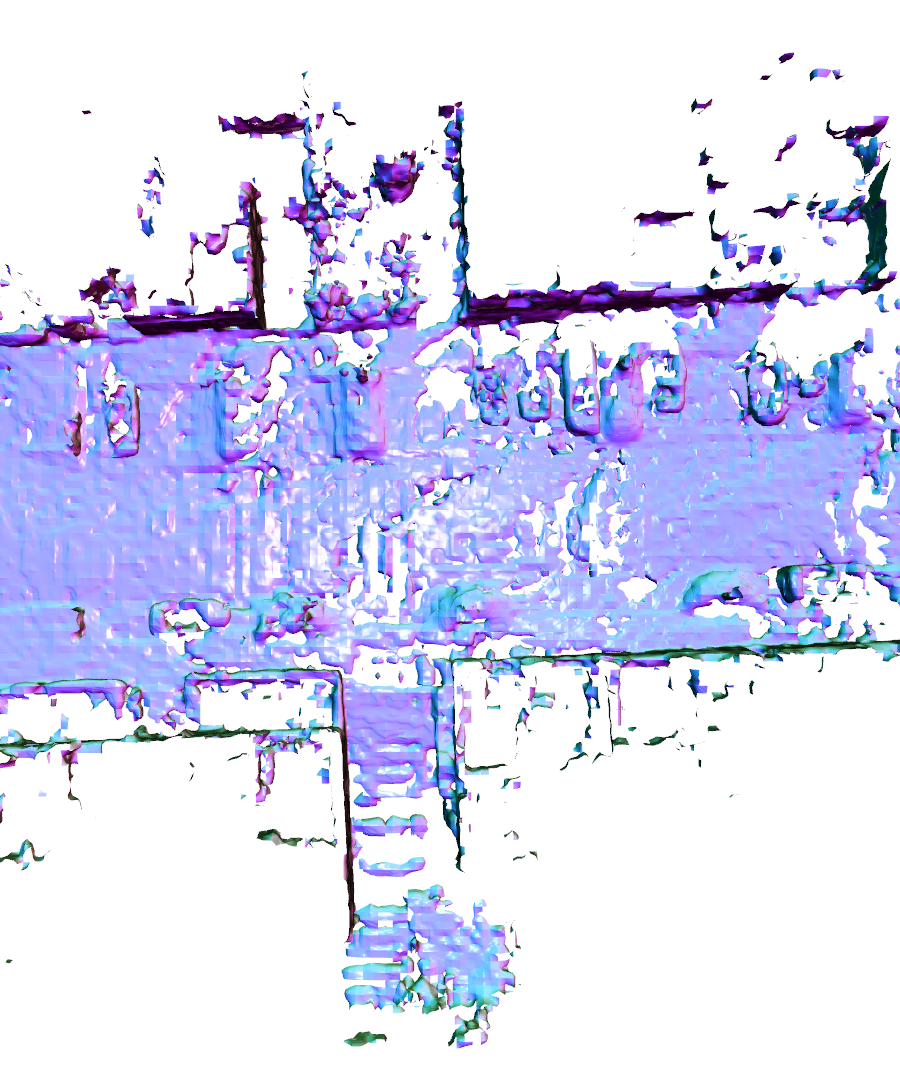
\includegraphics[width=1\linewidth]{figures/kittiwbce.png}
        \caption*{使用sdf loss与free-space loss}
	\end{minipage}
	\begin{minipage}{0.45\linewidth}
		\centering
		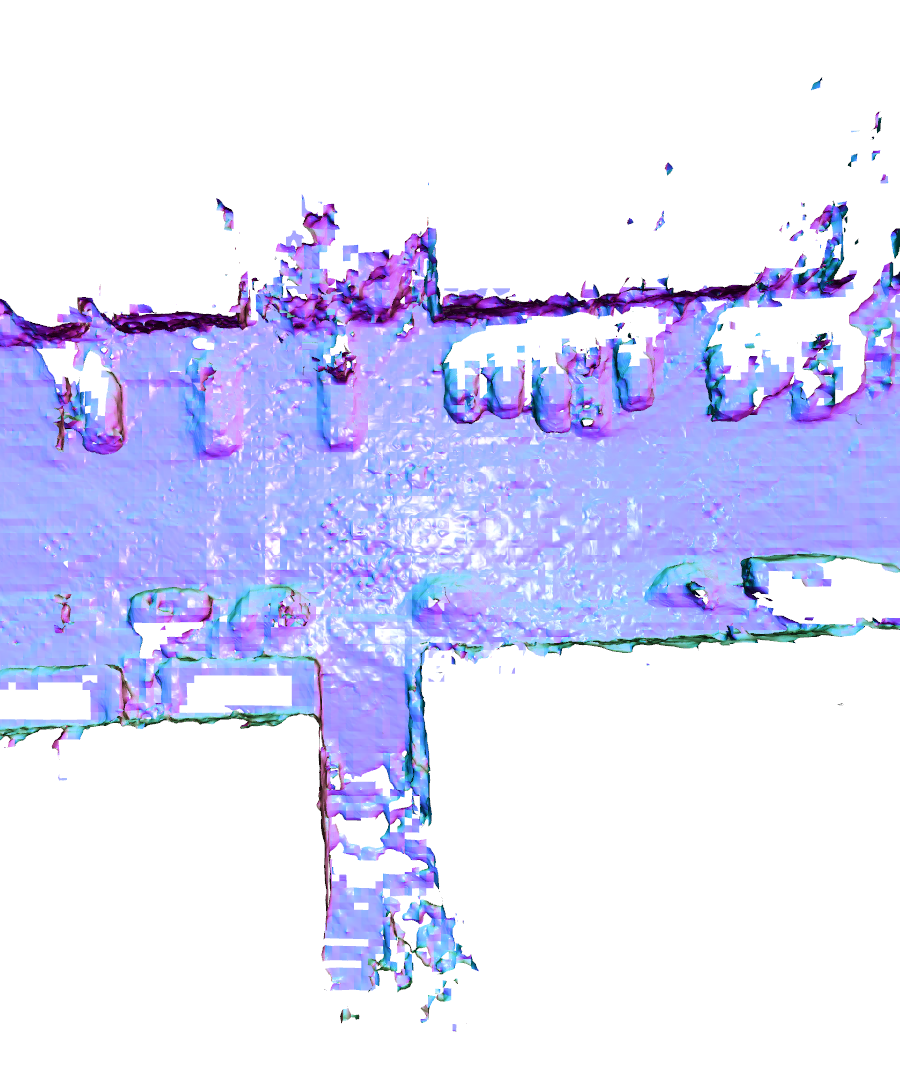
\includegraphics[width=1\linewidth]{figures/kittiobce.png}
        \caption*{使用二元交叉熵BCE loss}
	\end{minipage}
    \caption{在KITTI数据集上使用sdf loss与free-space loss和使用BCE loss的对比实验。左图结果显示特征网络和解码器并未精确学习到地图物体表面,所重建出的场景中地面与墙壁也远远不够平滑。当使用BCE loss对SDF值进行监督训练时,建图效果得到明显改善,如右图所示。}\label{becornot}
\end{figure}

同时本文使用式\ref{bce}中的二元交叉熵BCE loss和式\ref{voxloss}中sdf loss与free-space loss结合的方式进行了对比,在KITTI数据集上的结果如图\ref{becornot}所示。在左图中,将sdf loss与free-space loss设置相等的权重,结果显示网络并没有准确的学习到场景的表面信息,部分地图区域出现不连续的现象,且地面与墙壁的平滑度没有达到令人满意的程度。在右图中,关闭了对前两者损失函数的计算,只采用SDF的二元交叉熵函数对SDF值进行监督,可以看到地图的大部份表面处于连续状态,地面与墙壁等区域较为光滑。这说明网络较好的学习到了SDF值以复原出表面。

基于上述结果,可以得出在监督SDF训练时,使用Sigmoid函数将其映射到[0,1]的区间并使用二元交叉熵损失函数可以使网络更好的学习到场景表面。原因在于Sigmoid函数可以自动的为预测出的SDF值设置截断距离$tr$,以代替sdf loss。并且在物体的表面附近,也就是SDF值期望为0的区域, Sigmoid函数的梯度非常大,使得损失函数输出的结果显著,这也是训练过程中所期望的。
\clearpage
本文使用Voxblox和VDB Fusion,两种基于TSDF的传统视觉SLAM方法与SHINE-Mapping和 Vox-Fusion,两种基于神经隐式表达的建图方法在上述3种数据集上与本文方法进行了比较,该实验基于相同的分辨率配置。除Vox-Fusion外,其余三种方法均可在点云数据集上运行。本文将Vox-Fusion从读取RGB-D数据流扩展至点云数据输入。在3种数据集中, Mai City数据集和New College数据集拥有目标网格的Ground Truth数据,因此可以进行几何精度评估。此外,本文使用SemanticKITTI数据集进行了语义建图的精度评估。本文将实验结果分为无噪声的合成场景与更具挑战性的真实场景进行讨论。
\subsubsection{合成场景}
对于无噪声的合成数据集Mai City,本文使用3种基于神经网络隐式表达的建图方法在Seq01序列上进行实验。实验结果如图\ref{mairesult}所示。即使在无噪上的场景上,本文方法在细节部分仍优于Vox-Fusion,可以连续的保留车辆轮廓等细节信息。本文使用Mai City的Ground Truth网格数据对几何建图效果进行了评估,结果如表\ref{maicitymetric}所示。在各项指标上,本文方法优于Vox-Fusion。

\begin{figure}[htbp]
    \centering
    (a)
\begin{minipage}{0.322\linewidth}
    \centering
    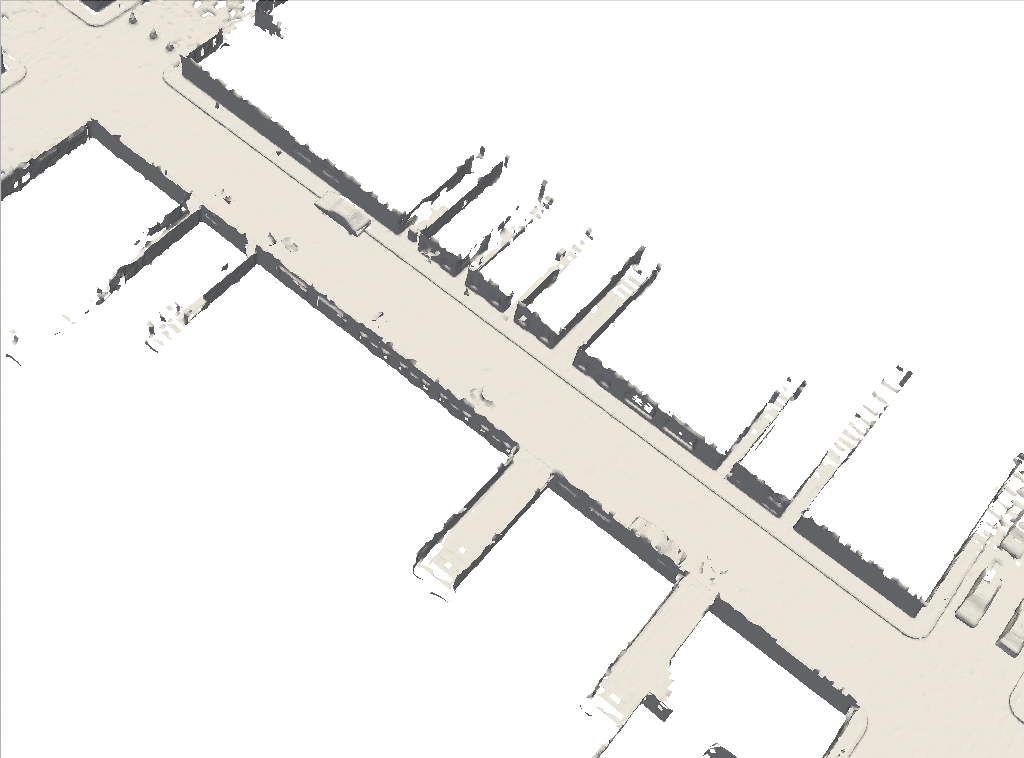
\includegraphics[width=1\linewidth]{figures/mai_3_vox.png}
\end{minipage}\hfill
\begin{minipage}{0.322\linewidth}
    \centering
    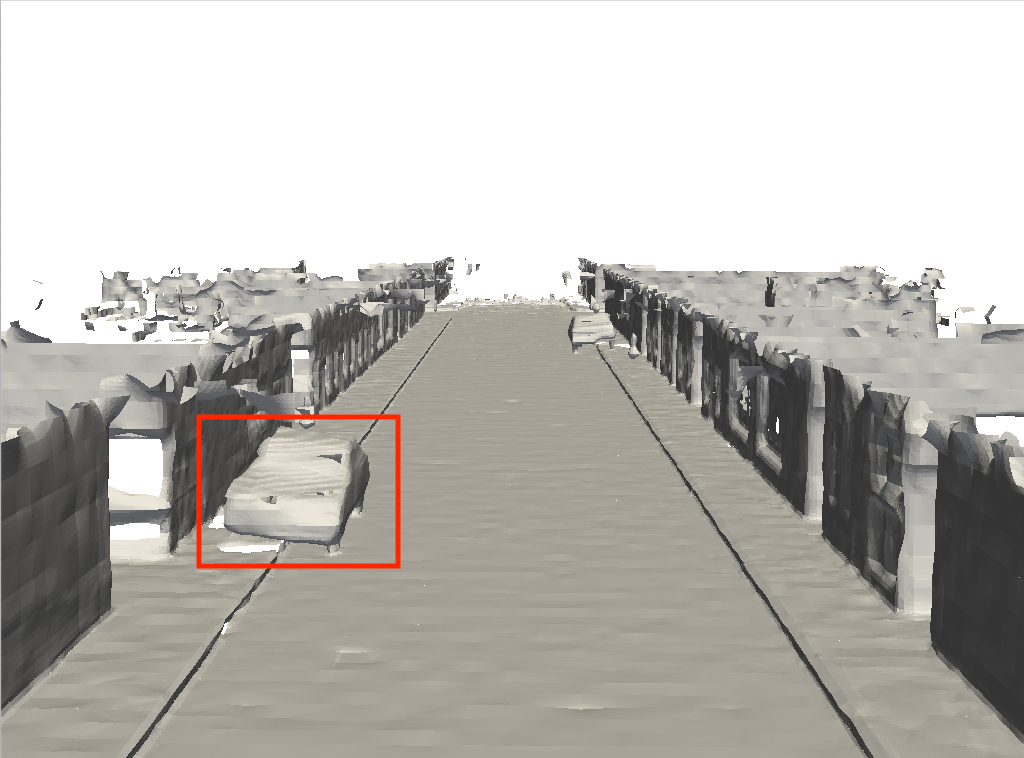
\includegraphics[width=1\linewidth]{figures/mai_1_vox.png}
\end{minipage}\hfill
\begin{minipage}{0.322\linewidth}
    \centering
    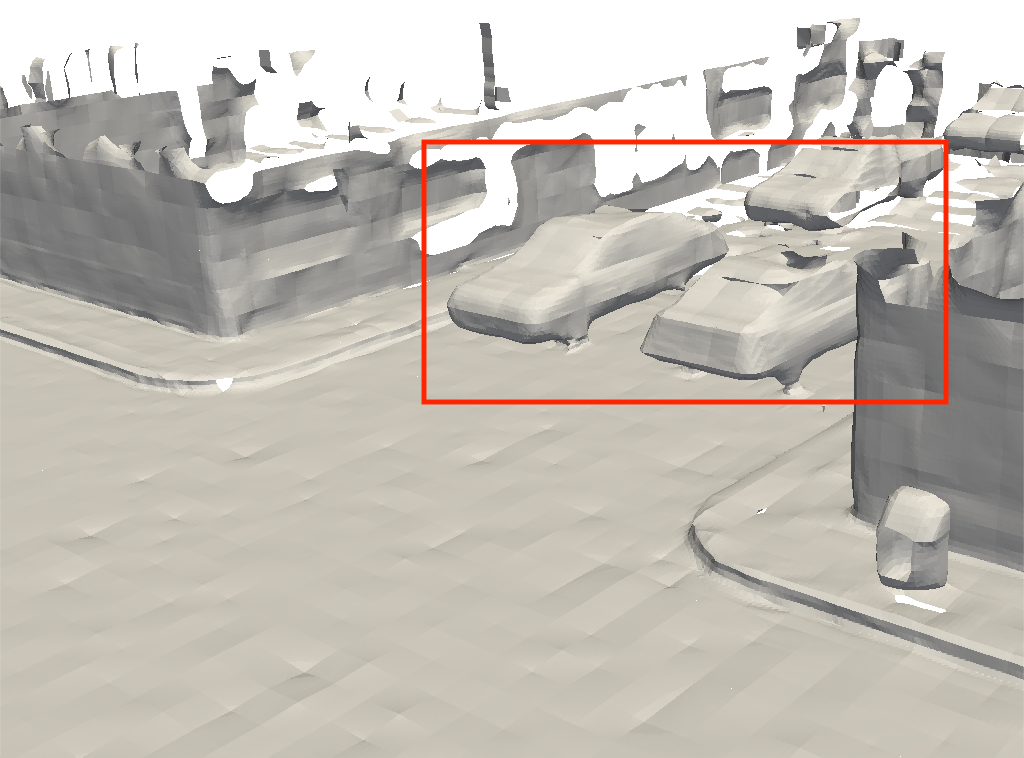
\includegraphics[width=1\linewidth]{figures/mai_2_vox.png}
\end{minipage}\vfill
(b)
\begin{minipage}{0.322\linewidth}
    \centering
    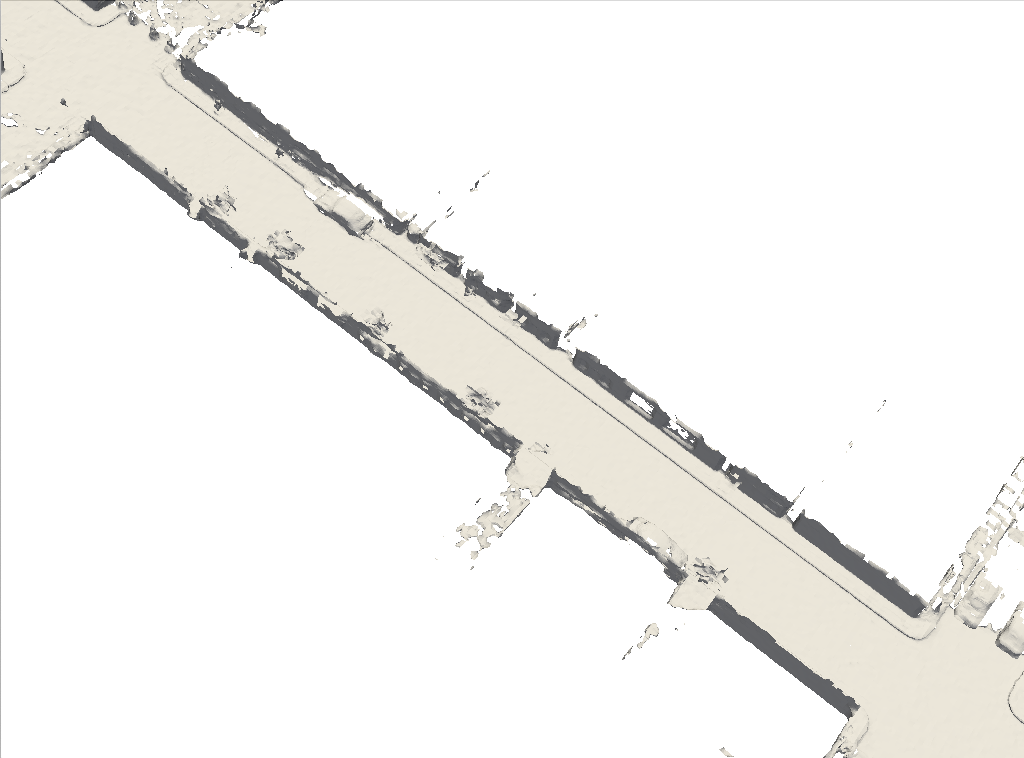
\includegraphics[width=1\linewidth]{figures/mai_3_bce.png}
\end{minipage}\hfill
\begin{minipage}{0.322\linewidth}
    \centering
    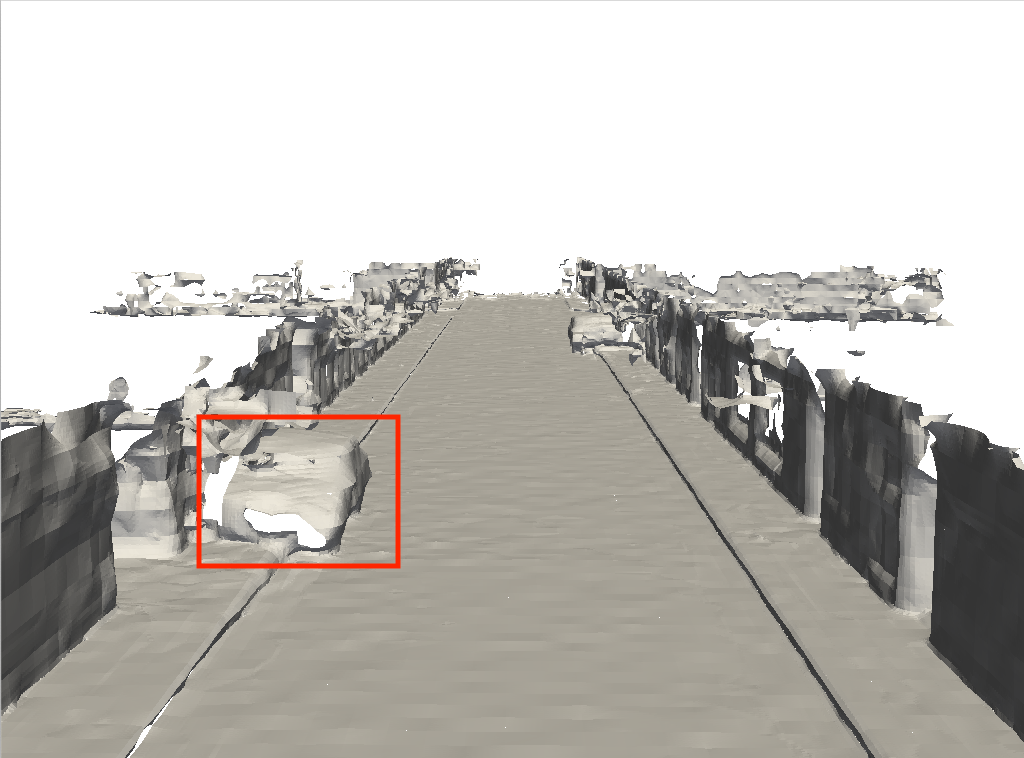
\includegraphics[width=1\linewidth]{figures/mai_1_bce.png}
\end{minipage}\hfill
\begin{minipage}{0.322\linewidth}
    \centering
    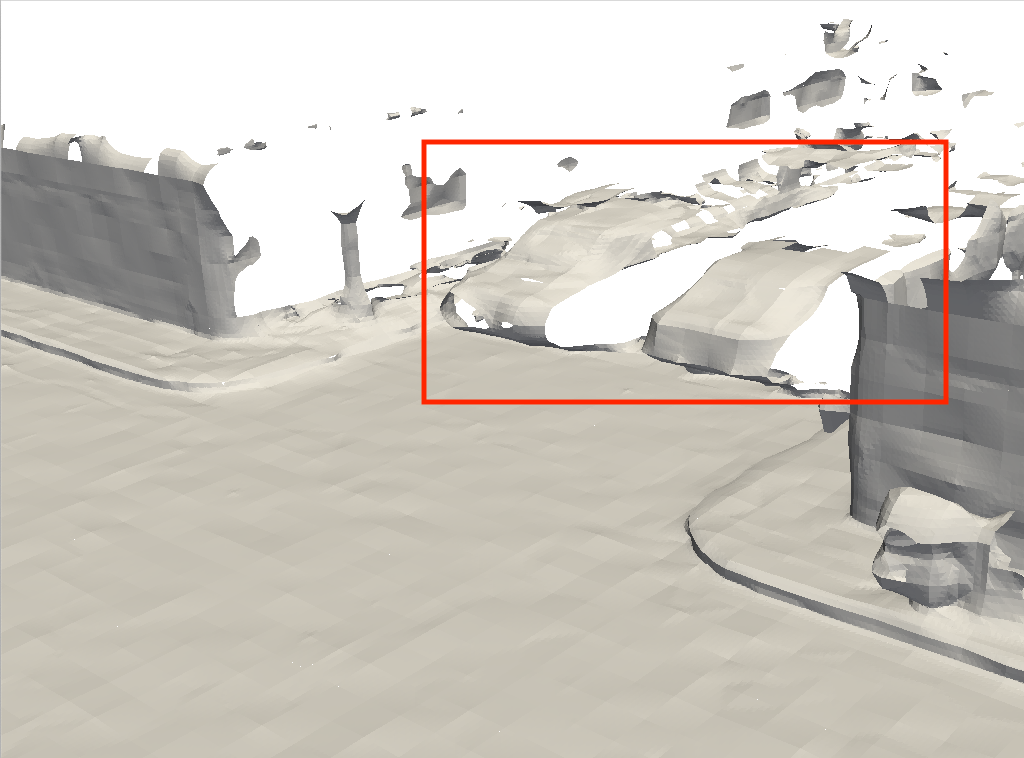
\includegraphics[width=1\linewidth]{figures/mai_2_bce.png}
\end{minipage}\vfill
(c)
\begin{minipage}{0.322\linewidth}
    \centering
    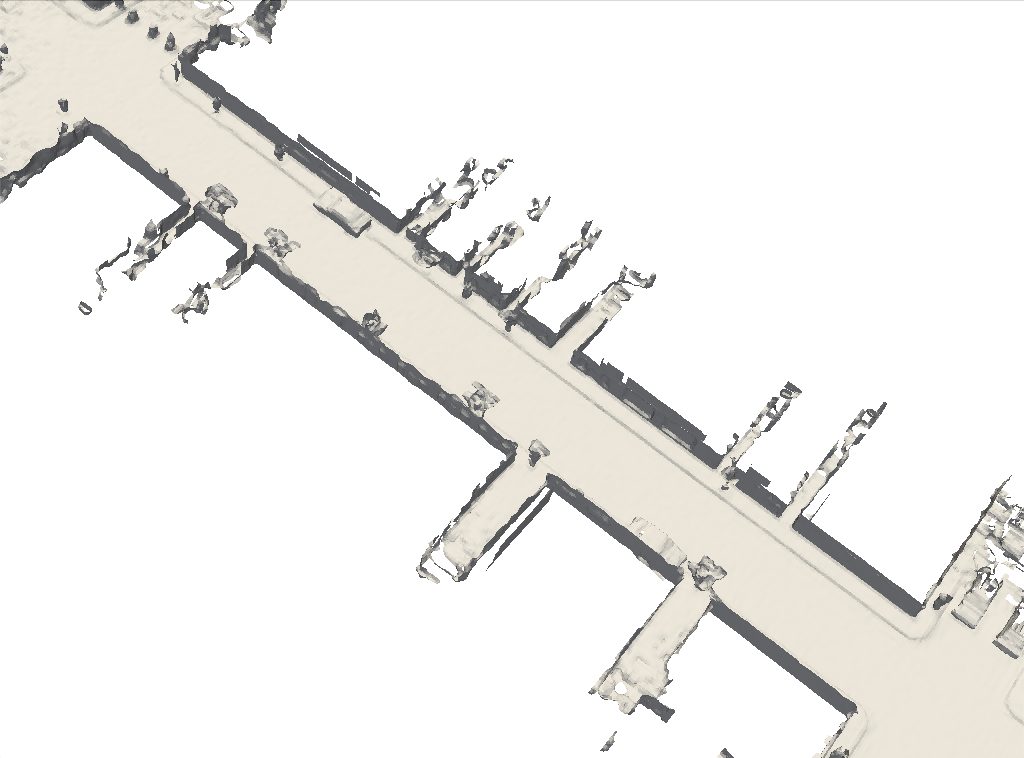
\includegraphics[width=1\linewidth]{figures/mai_3_shine.png}
    \end{minipage}\hfill
    \begin{minipage}{0.322\linewidth}
    \centering
    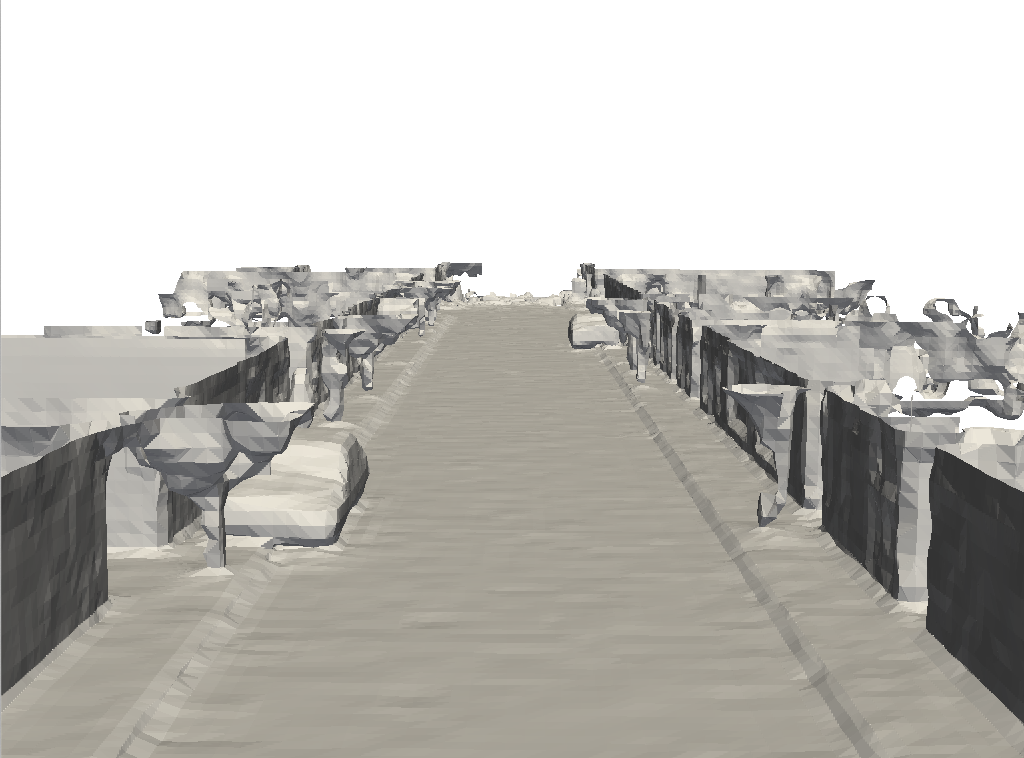
\includegraphics[width=1\linewidth]{figures/mai_1_shine.png}
    \end{minipage}\hfill
    \begin{minipage}{0.322\linewidth}
    \centering
    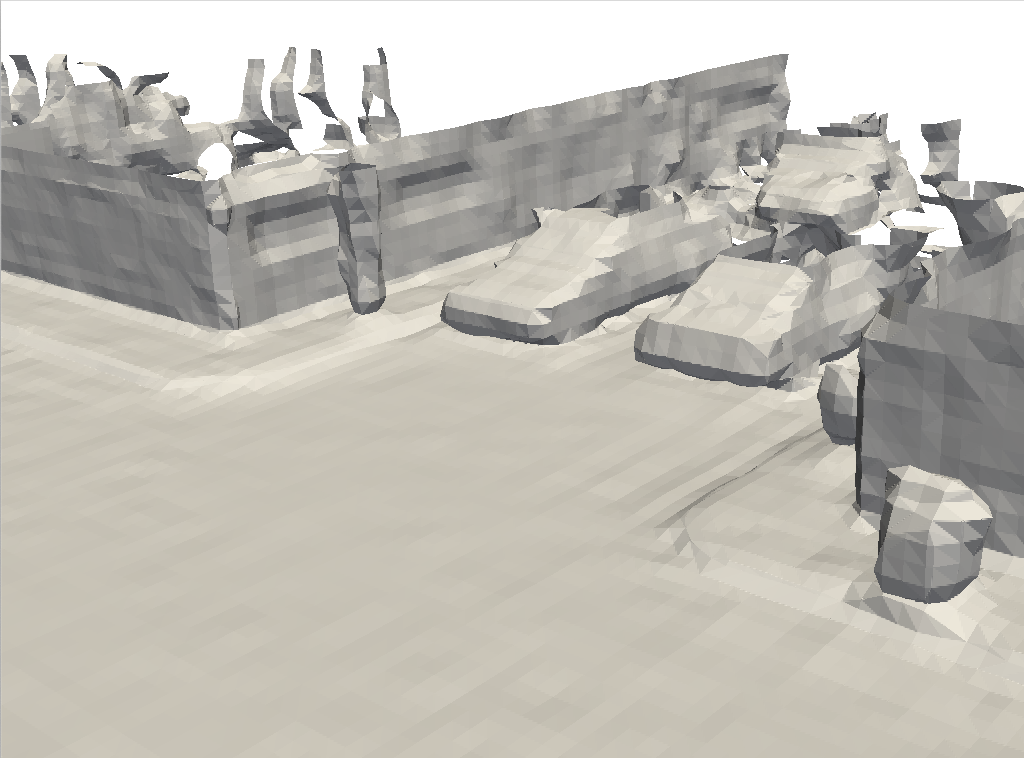
\includegraphics[width=1\linewidth]{figures/mai_2_shine.png}
    \end{minipage}
\caption{3种基于神经网络的隐式建图方法在Mai City数据集上的结果。分别为(a)本文方法, (b)Vox-Fusion与(c)SHINE-Mapping。}\label{mairesult}
\end{figure}

\begin{table}[htbp]
    \centering
    \caption{定性测量的不同方法在Mai City数据集上建图的几何精度,将目标地图与重建地图之间对应点重合的阈值$threshold$设置为10cm。}\label{maicitymetric}
    \begin{tabular}[htbp]{llccccc}
        \toprule
        \multicolumn{2}{l}{方法} & $\mathbf{Comp.}$(cm) & $\mathbf{Acc.}(\%)$ & $\mathbf{C-l1}$(cm) &  $\mathbf{Comp. Ratio}$(\%) &$\mathbf{F1-score}$\\
        \midrule
        \multicolumn{2}{l}{Voxblox} & 7.1 & 93.3 & 4.8 &84.0&90.0\\
        \multicolumn{2}{l}{VDB Fusion} & 6.9&92.1&4.5&90.2&94.1 \\
        \multicolumn{2}{l}{SHINE-Mapping} & 3.2&94.6&2.9&95.2&95.9 \\
        \multicolumn{2}{l}{Vox-Fusion} & 18.0 & 90.3 &11.2&76.3&82.8\\
        \midrule
        \multicolumn{2}{l}{Ours+bce} & 12.5&95.2 &8.3&85.7&90.2\\
        \bottomrule
    \end{tabular}
\end{table}
\subsubsection{真实场景}
本文使用5种方法在KITTI数据集Seq00序列的前200帧上进行建图。实验结果如图\ref{kittiresult}所示。可以看到本文方法在建图效果上媲美SHINE-Mapping与VDB Fusion,以相同的建图速度和更低的分辨率达到了相同的效果。本文使用的优化方法在地图细节处理上效果优于Vox-Fusion,如车辆,墙壁等细节。实验证明本文方法可以在真实无人驾驶数据集上对室外大规模地图进行实时建图,在保留细节的同时保持地图的连续性。
\begin{figure}[htbp]
	\centering
    (a)
	\begin{minipage}{0.322\linewidth}
		\centering
		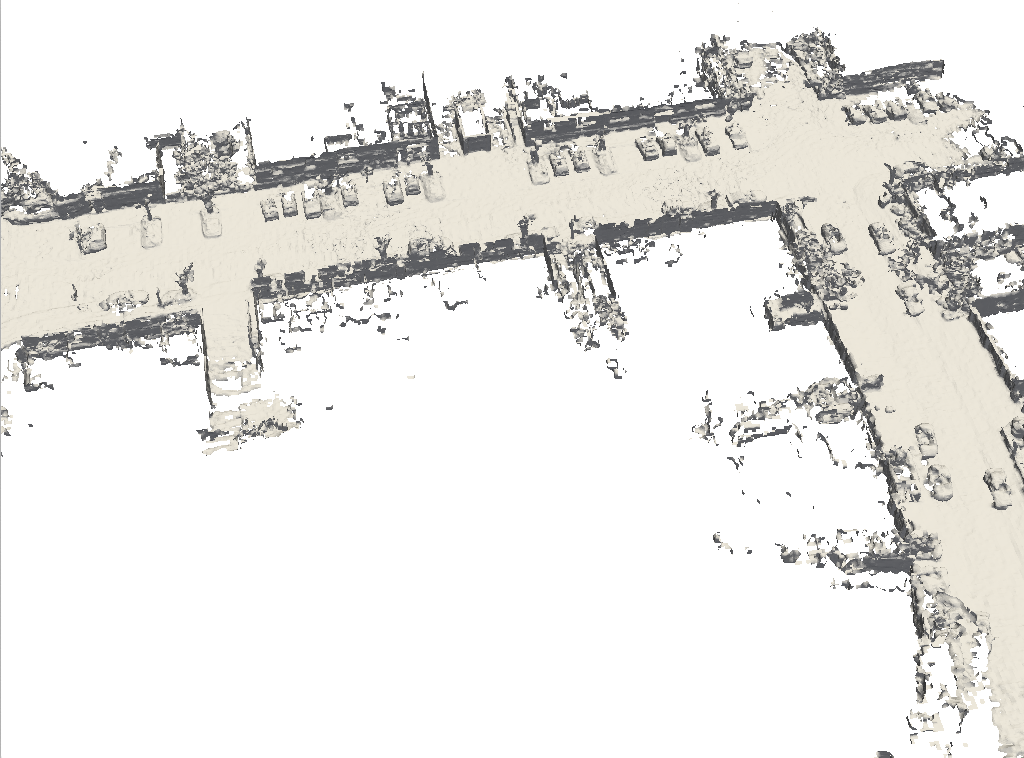
\includegraphics[width=1\linewidth]{figures/kitti_1_vox.png}
	\end{minipage}\hfill
	\begin{minipage}{0.322\linewidth}
		\centering
		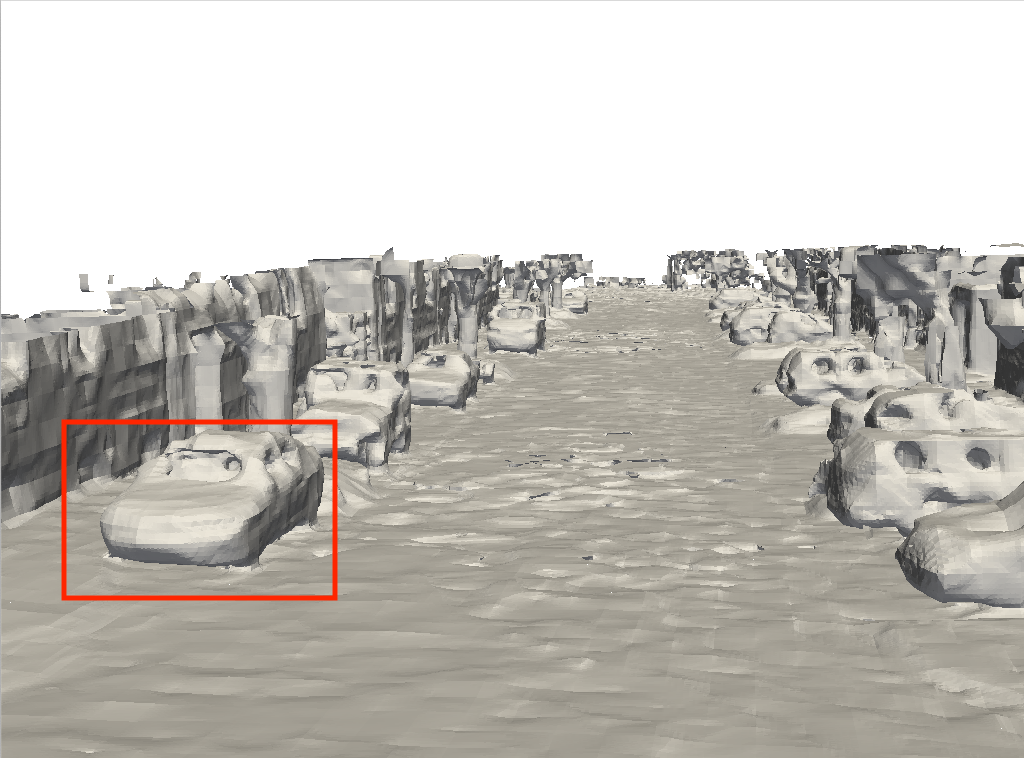
\includegraphics[width=1\linewidth]{figures/kitti_2_vox.png}
	\end{minipage}\hfill
    \begin{minipage}{0.322\linewidth}
		\centering
		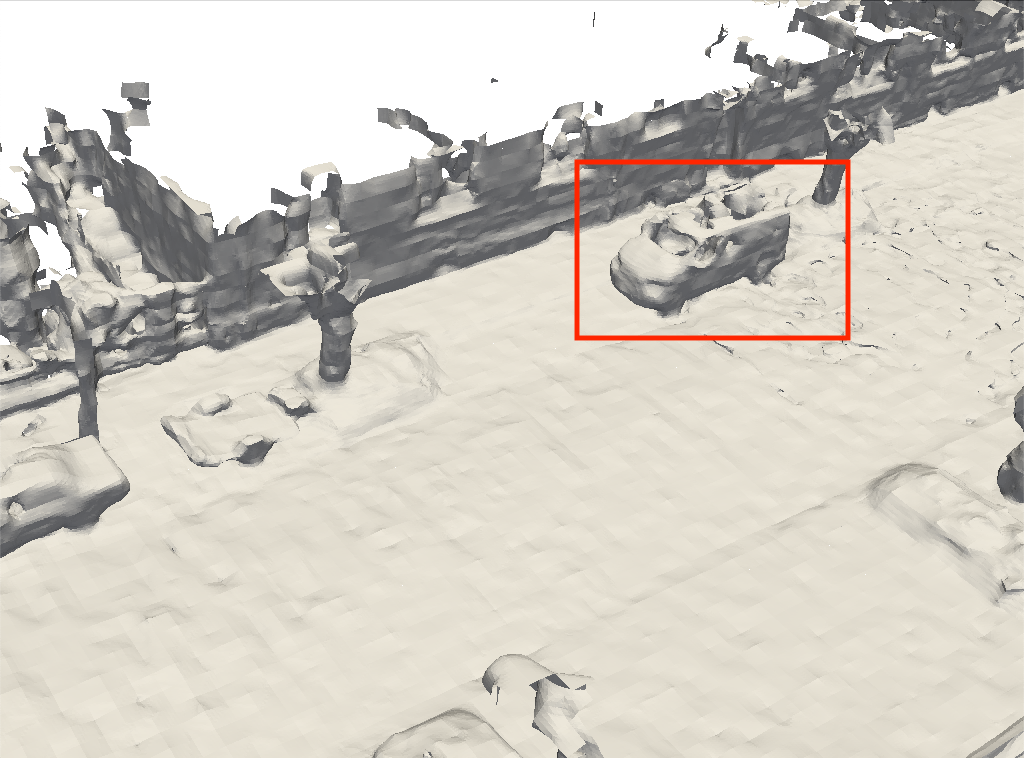
\includegraphics[width=1\linewidth]{figures/kitti_3_vox.png}
	\end{minipage}\vfill
    (b)
	\begin{minipage}{0.322\linewidth}
		\centering
		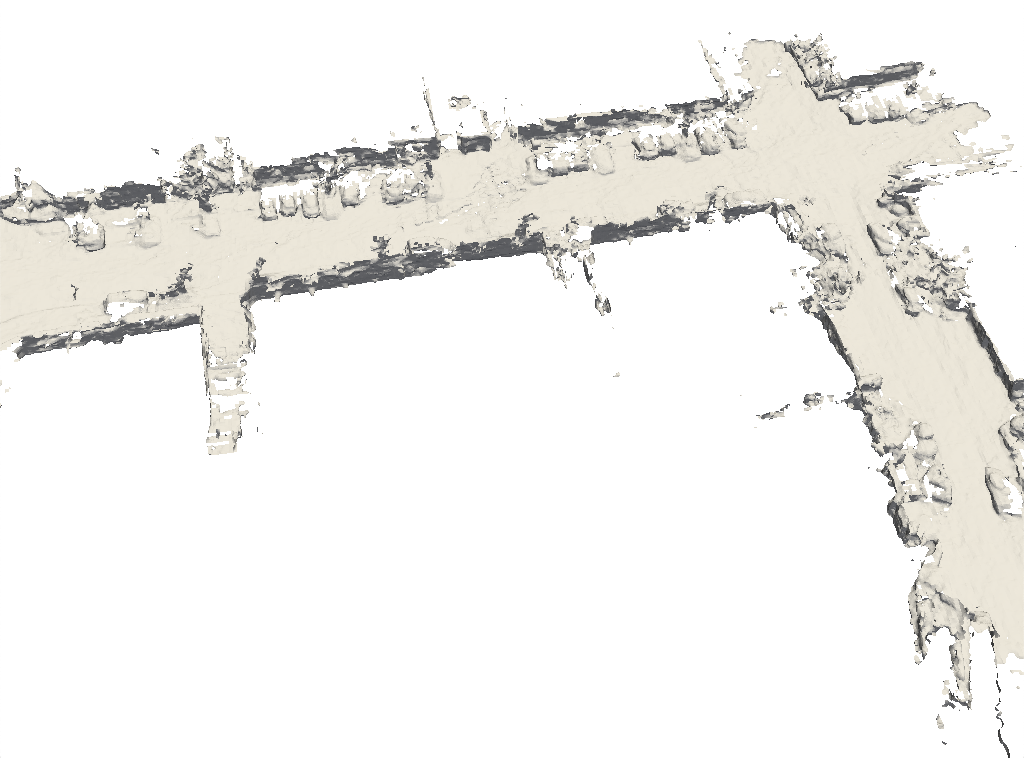
\includegraphics[width=1\linewidth]{figures/kitti_1_bce.png}
	\end{minipage}\hfill
	\begin{minipage}{0.322\linewidth}
		\centering
		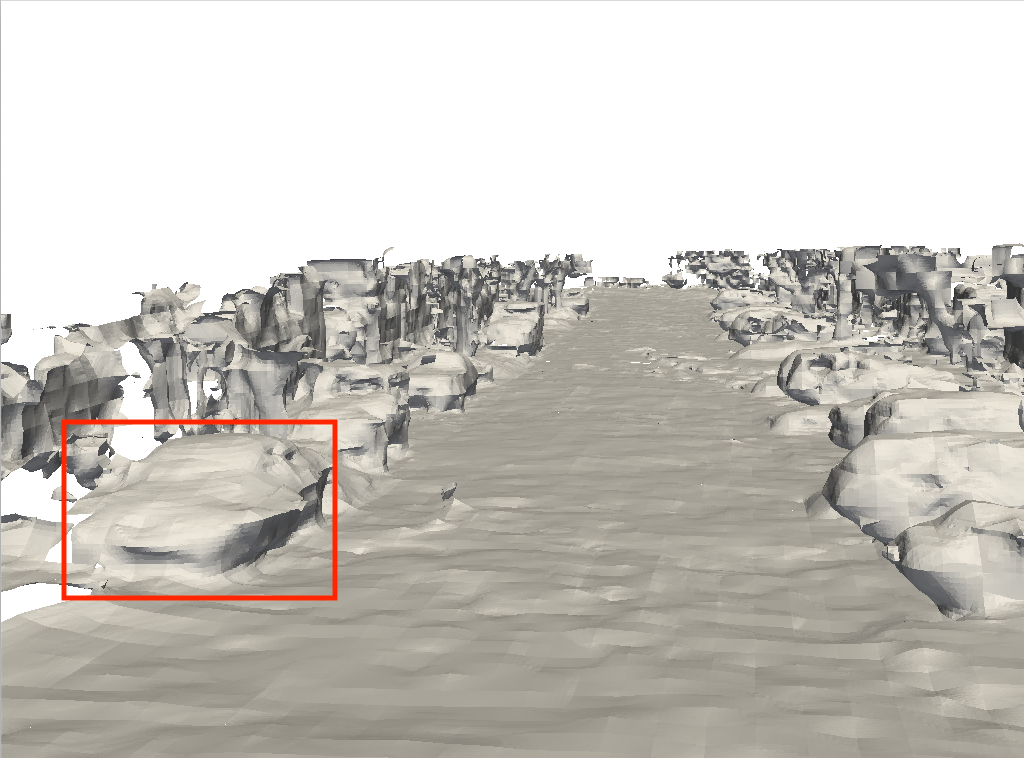
\includegraphics[width=1\linewidth]{figures/kitti_2_bce.png}
	\end{minipage}\hfill
    \begin{minipage}{0.322\linewidth}
		\centering
		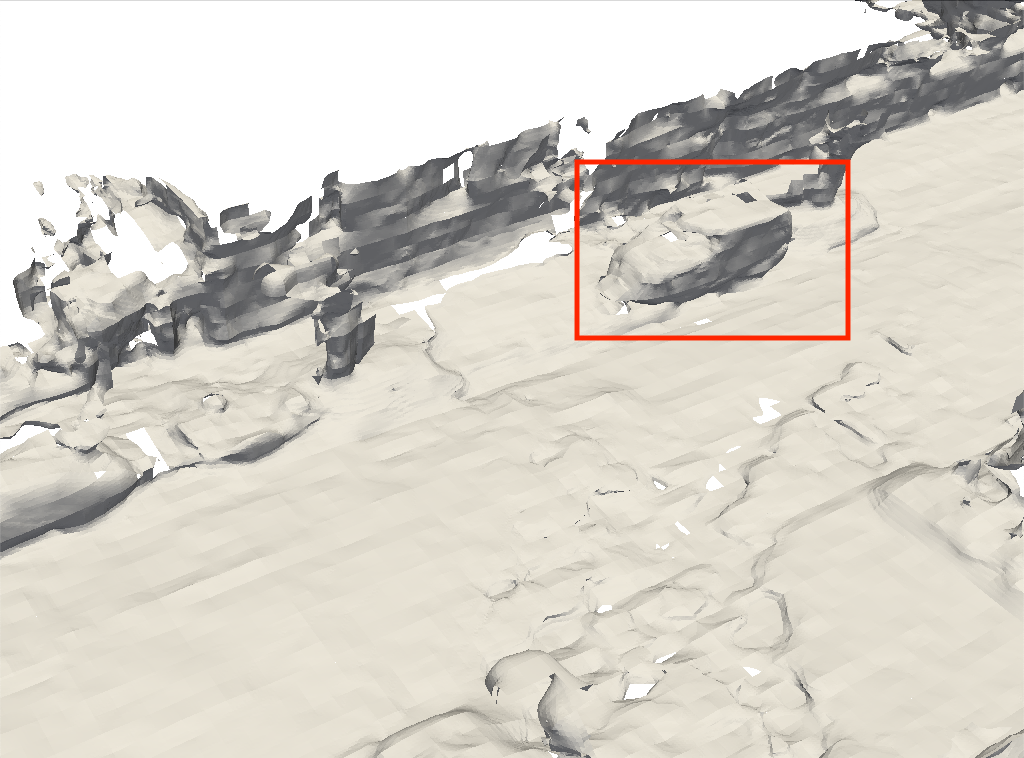
\includegraphics[width=1\linewidth]{figures/kitti_3_bce.png}
	\end{minipage}\vfill
    (c)
    \begin{minipage}{0.322\linewidth}
		\centering
		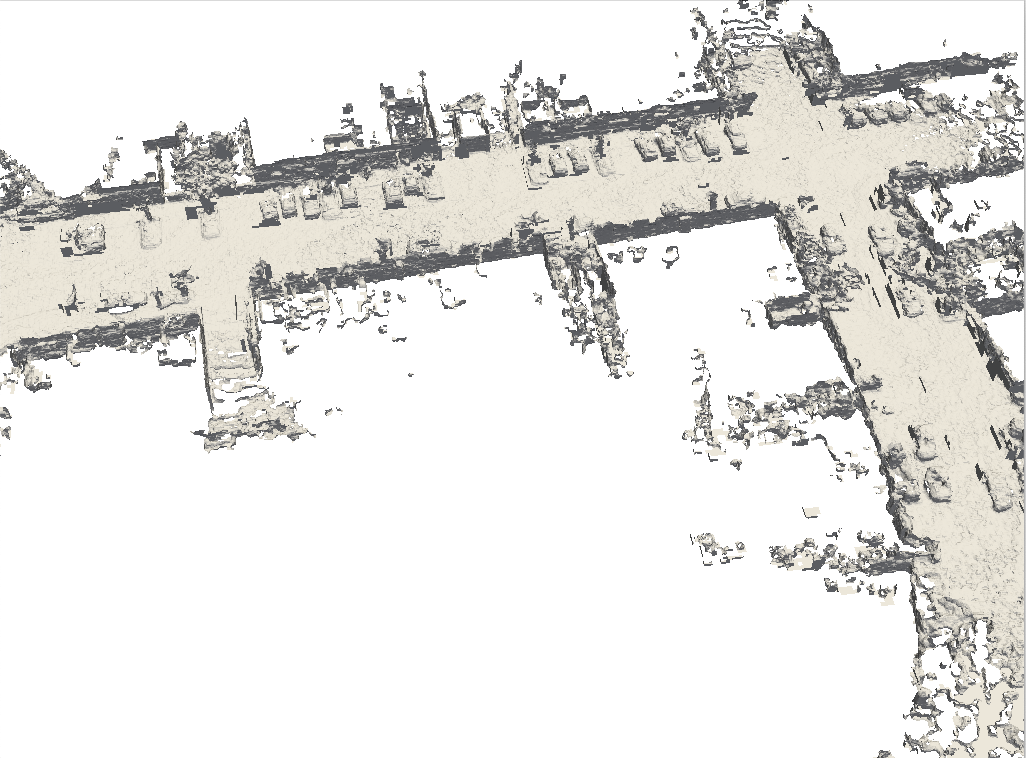
\includegraphics[width=1\linewidth]{figures/kitti_1_shine.png}
	\end{minipage}\hfill
	\begin{minipage}{0.322\linewidth}
		\centering
		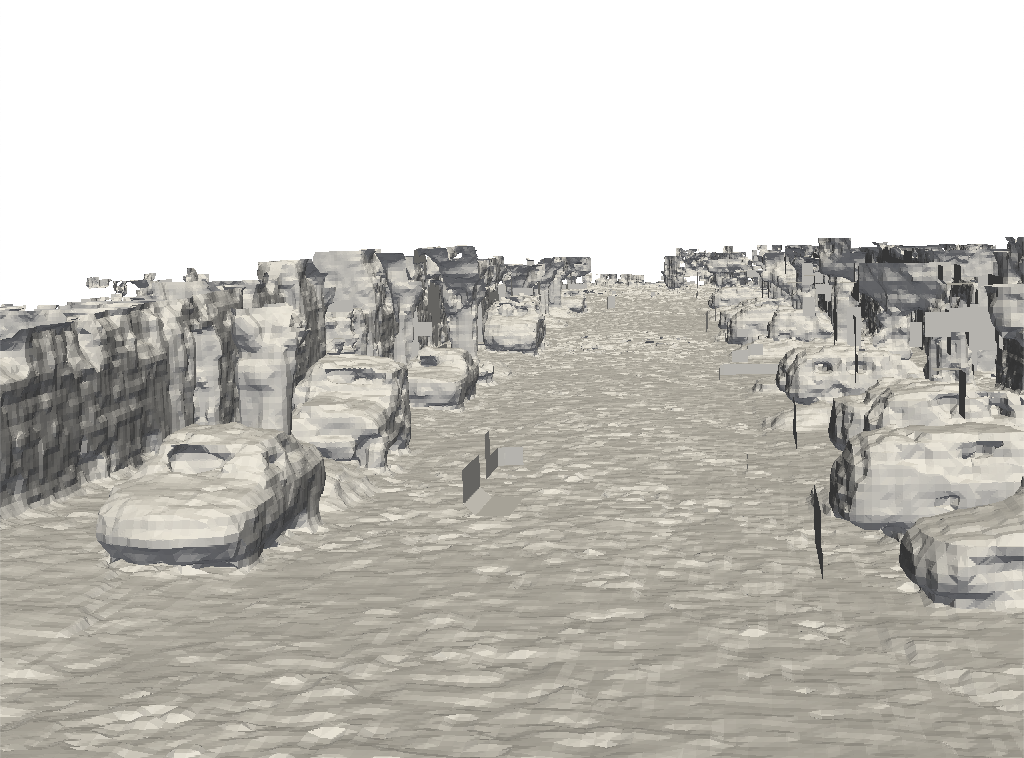
\includegraphics[width=1\linewidth]{figures/kitti_2_shine.png}
	\end{minipage}\hfill
    \begin{minipage}{0.322\linewidth}
		\centering
		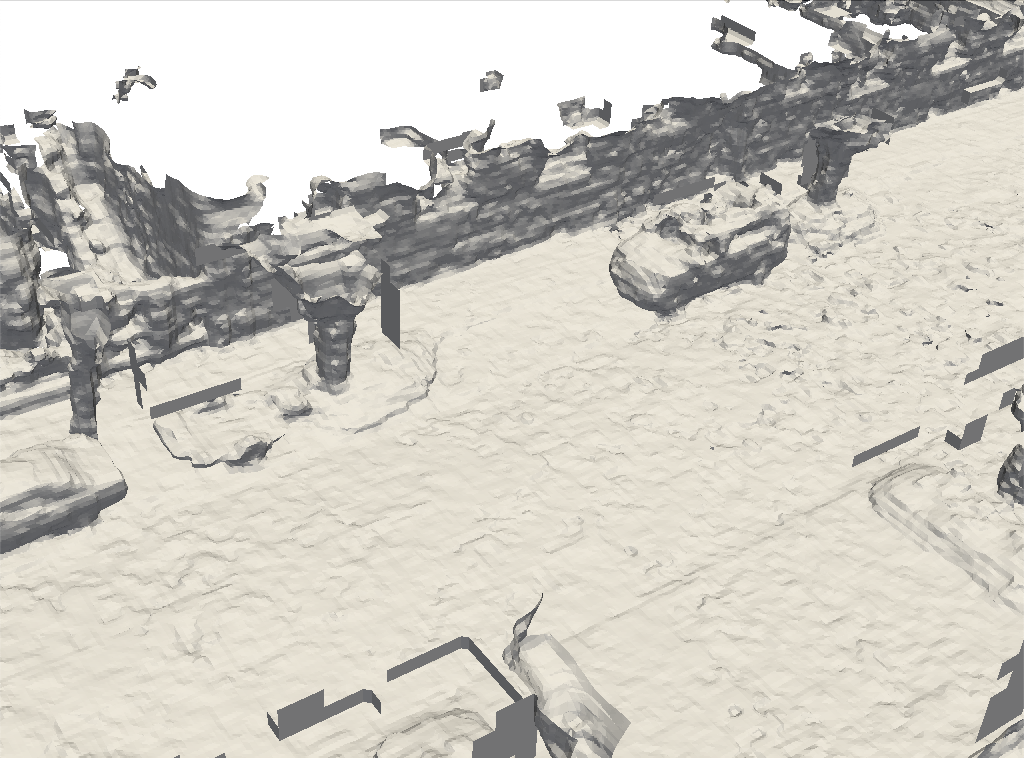
\includegraphics[width=1\linewidth]{figures/kitti_3_shine.png}
	\end{minipage}\vfill
    (d)
	\begin{minipage}{0.322\linewidth}
		\centering
		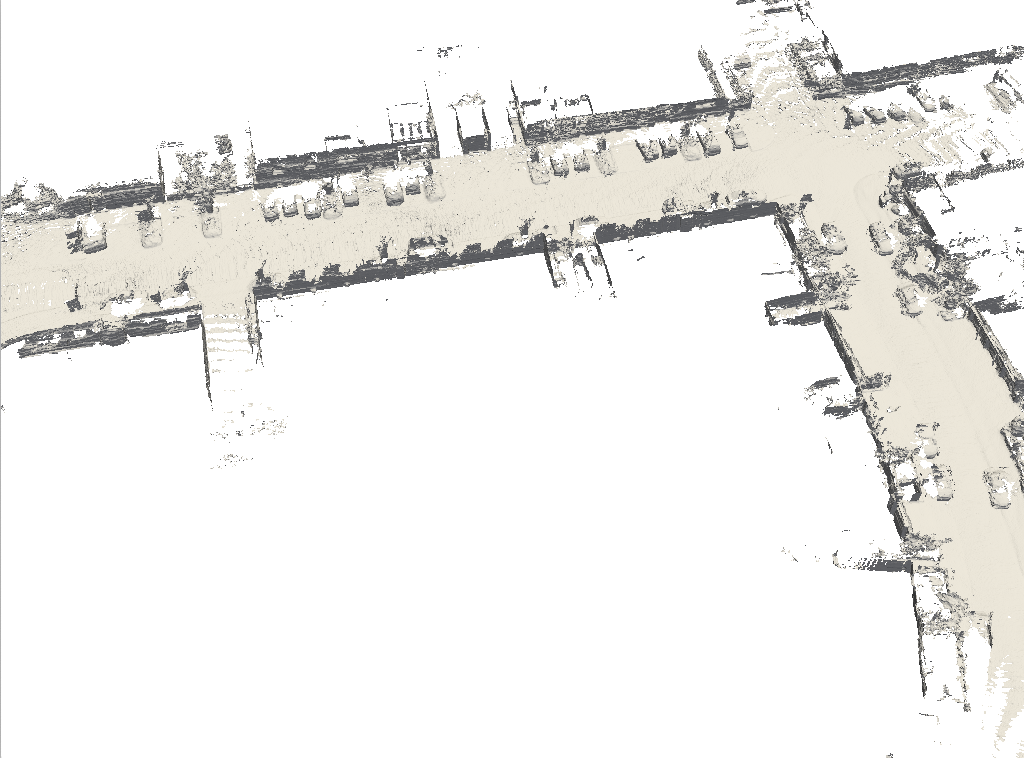
\includegraphics[width=1\linewidth]{figures/kitti_1_vdb.png}
	\end{minipage}\hfill
	\begin{minipage}{0.322\linewidth}
		\centering
		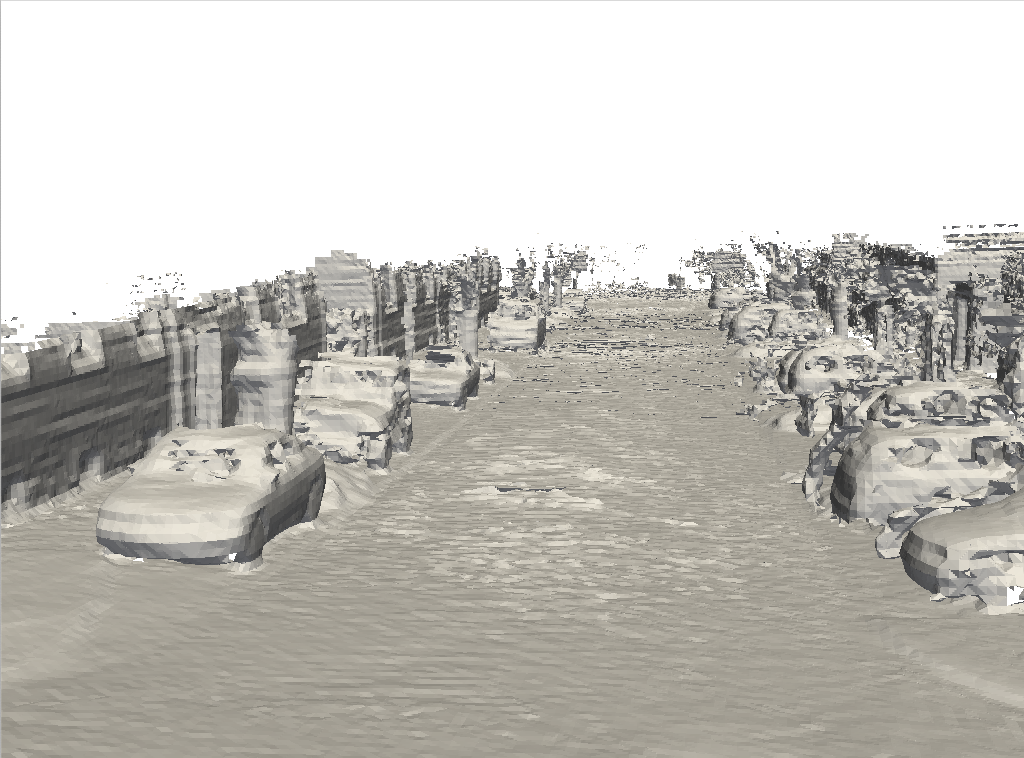
\includegraphics[width=1\linewidth]{figures/kitti_2_vdb.png}
	\end{minipage}\hfill
    \begin{minipage}{0.322\linewidth}
		\centering
		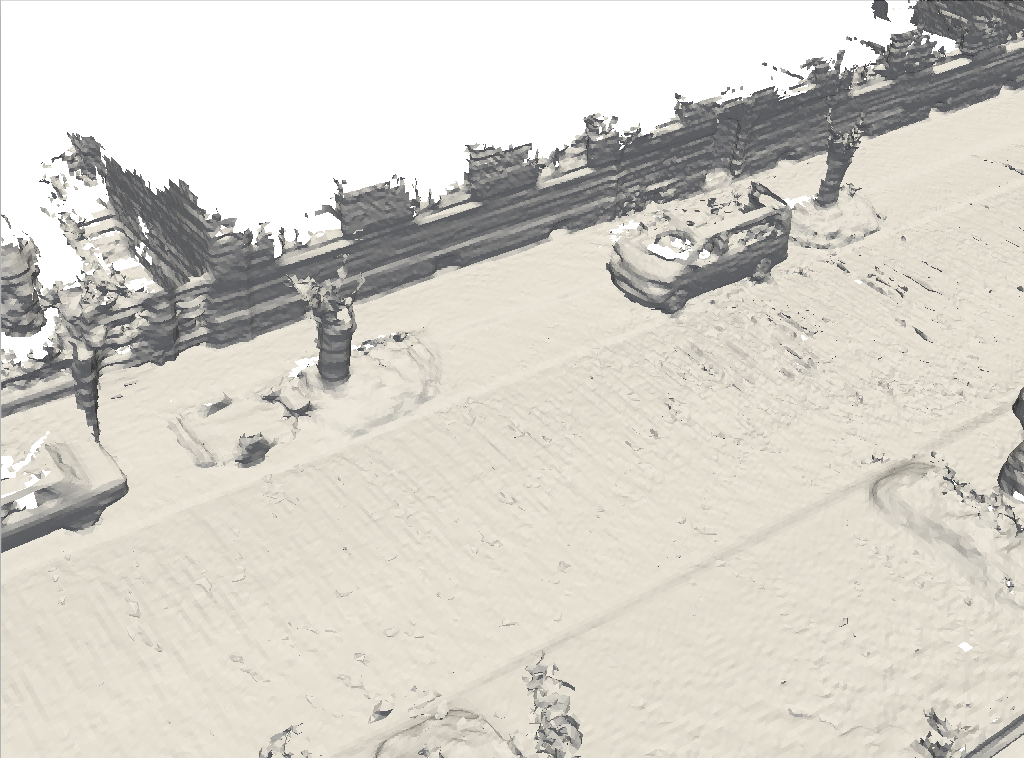
\includegraphics[width=1\linewidth]{figures/kitti_3_vdb.png}
	\end{minipage}\vfill
    (e)
    \begin{minipage}{0.322\linewidth}
        \centering
        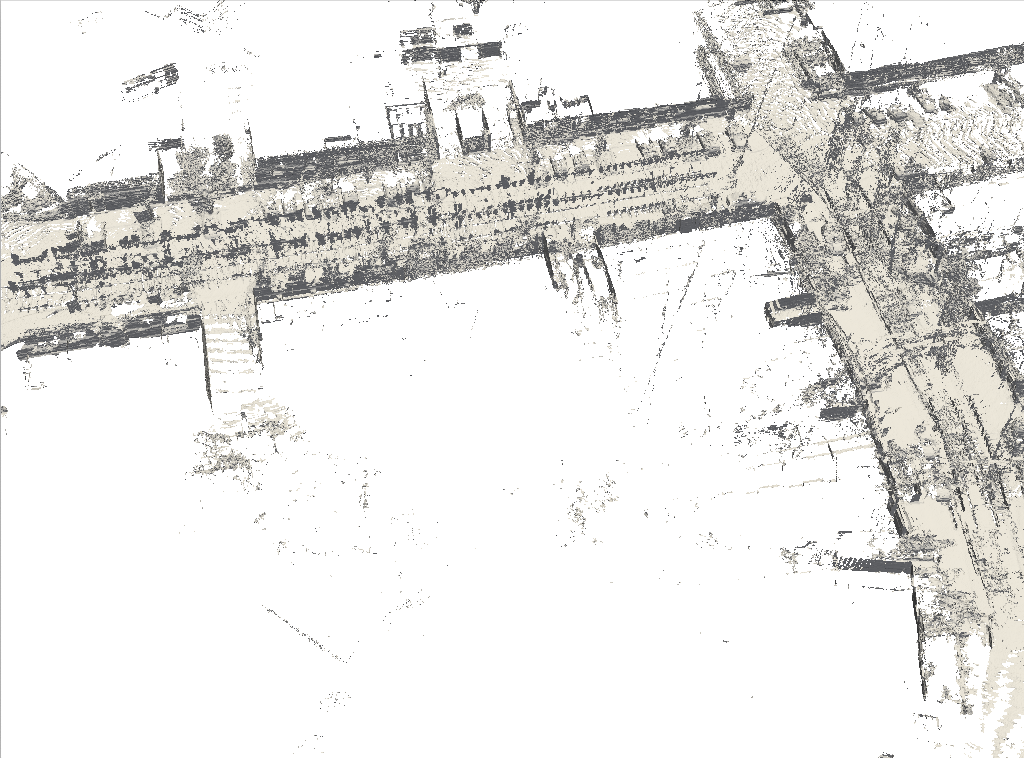
\includegraphics[width=1\linewidth]{figures/kitti_1_voxblox.png}
        \end{minipage}\hfill
        \begin{minipage}{0.322\linewidth}
        \centering
        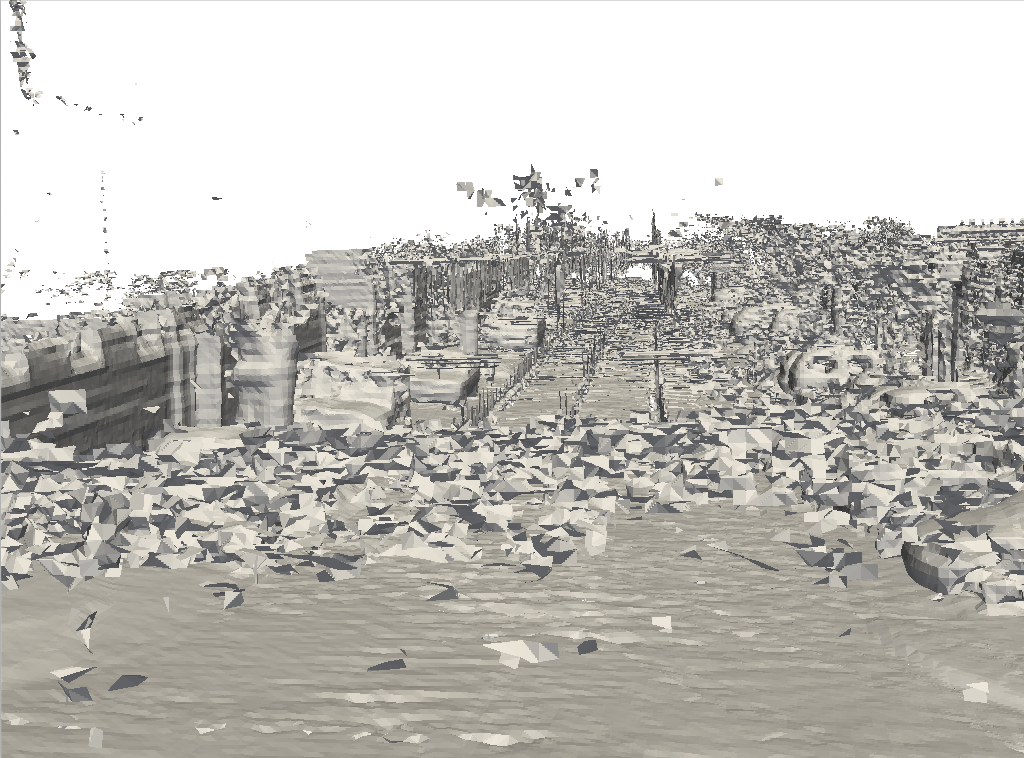
\includegraphics[width=1\linewidth]{figures/kitti_2_voxblox.png}
        \end{minipage}\hfill
        \begin{minipage}{0.322\linewidth}
        \centering
        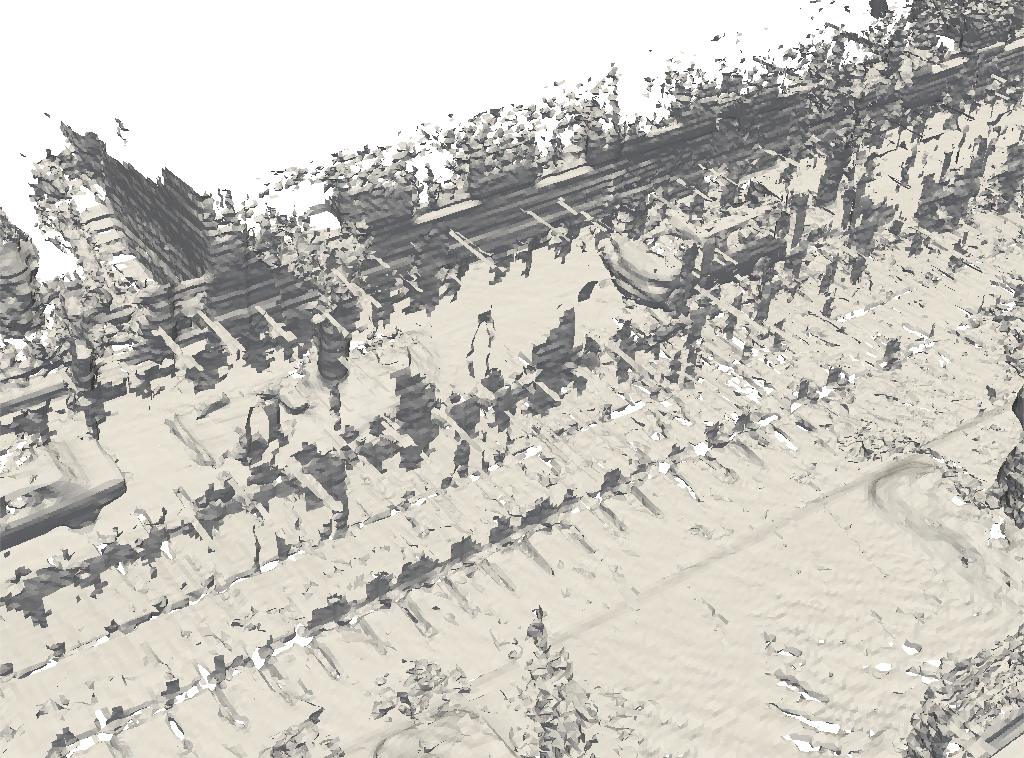
\includegraphics[width=1\linewidth]{figures/kitti_3_voxblox.png}
        \end{minipage}
    \caption{5种不同方法在KITTI数据集Seq00序列上的结果。分别为(a)本文方法, (b)Vox-Fusion, (c)SHINE-Mapping, (d)VDB Fusion与(e)Voxblox}\label{kittiresult}
\end{figure}

同样的,本文使用3种基于神经隐式表达的建图方法在New College数据集的Seq01序列上进行了实验实验结果如图\ref{ncdresult}所示。在具有更多噪声的场景中建图是具有挑战性的,所有方法的效果均低于在合成场景与相对噪声较小的真实场景。由于该数据集拥有网格地图的真实数据,本文对其几何建图精度进行了评估,结果如表\ref{ncdmetric}所示。由于噪声较大,该评估将阈值$threshold$设置为20cm。本文算法在几何精度指标上与SHINE-Mapping相近,效果远优于Vox-Fusion。
\begin{figure}[htbp]
    \centering
    (a)
\begin{minipage}{0.322\linewidth}
    \centering
    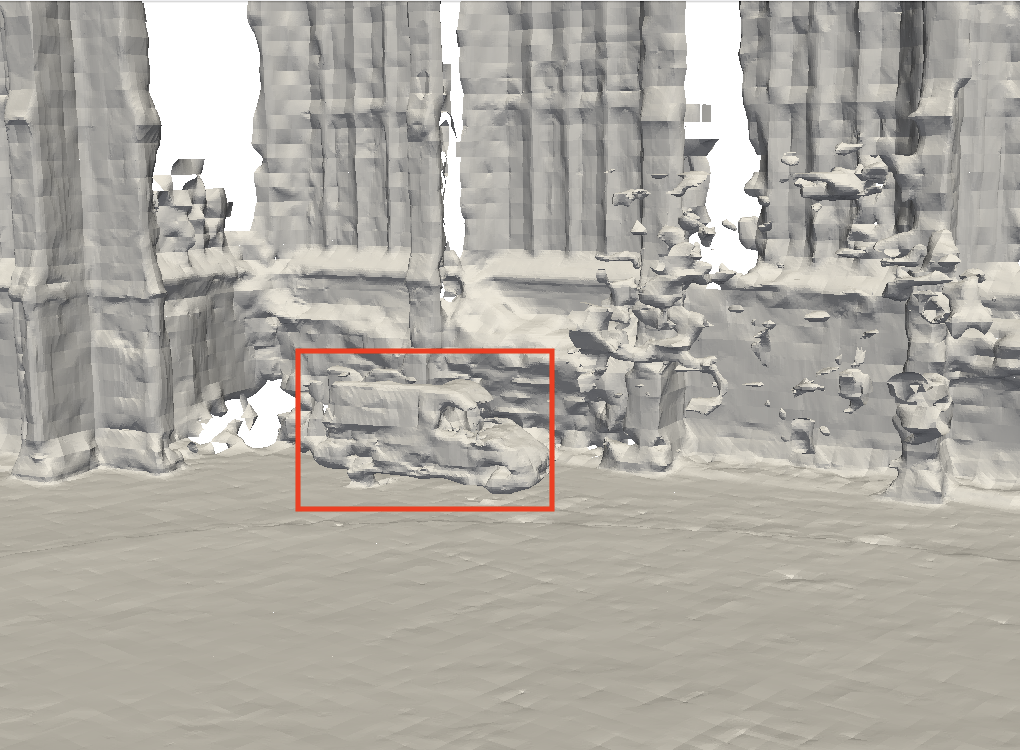
\includegraphics[width=1\linewidth]{figures/ncd_3_vox.png}
\end{minipage}\hfill
\begin{minipage}{0.322\linewidth}
    \centering
    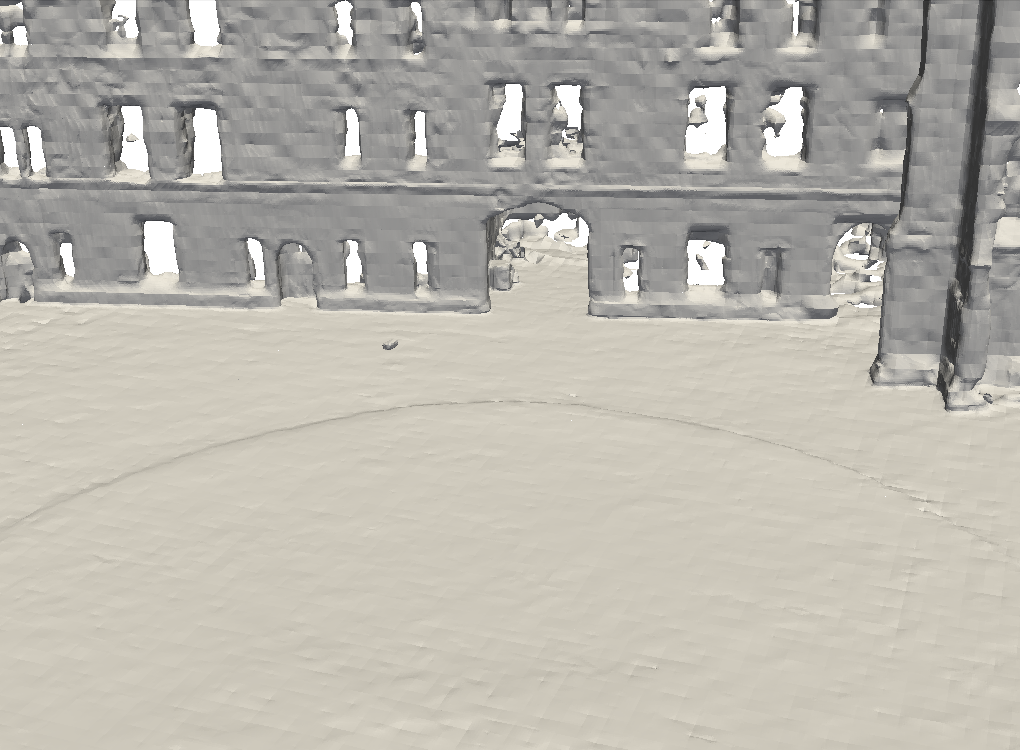
\includegraphics[width=1\linewidth]{figures/ncd_2_vox.png}
\end{minipage}\hfill
\begin{minipage}{0.322\linewidth}
    \centering
    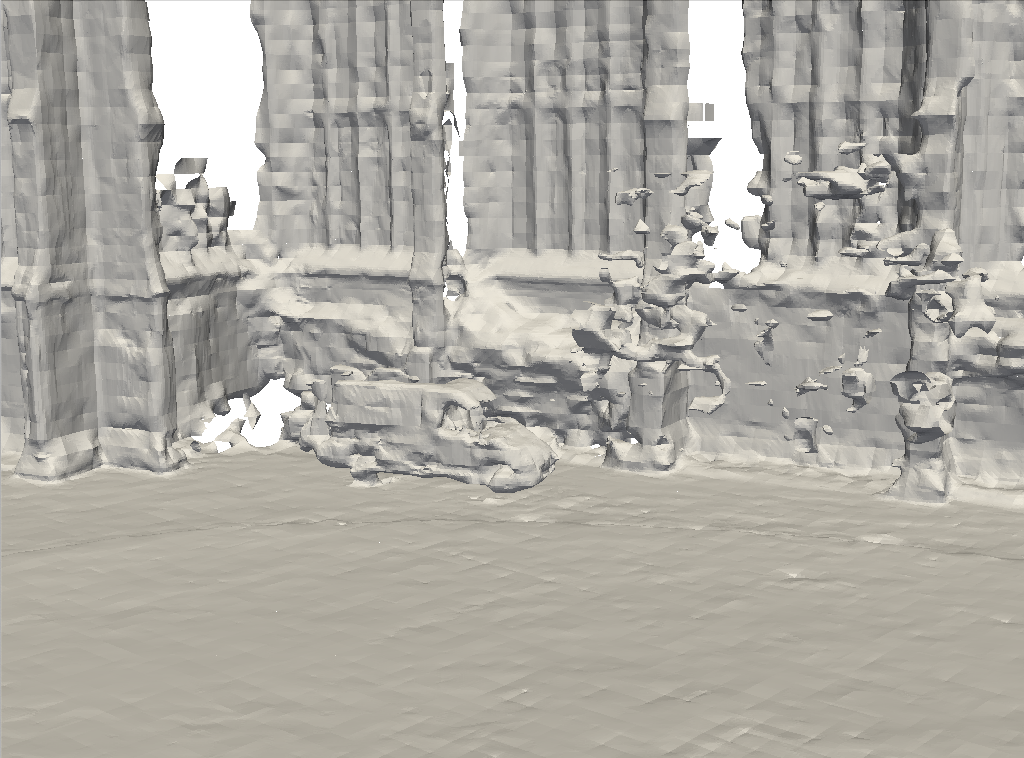
\includegraphics[width=1\linewidth]{figures/ncd_1_vox.png}
\end{minipage}\vfill
(b)
\begin{minipage}{0.322\linewidth}
    \centering
    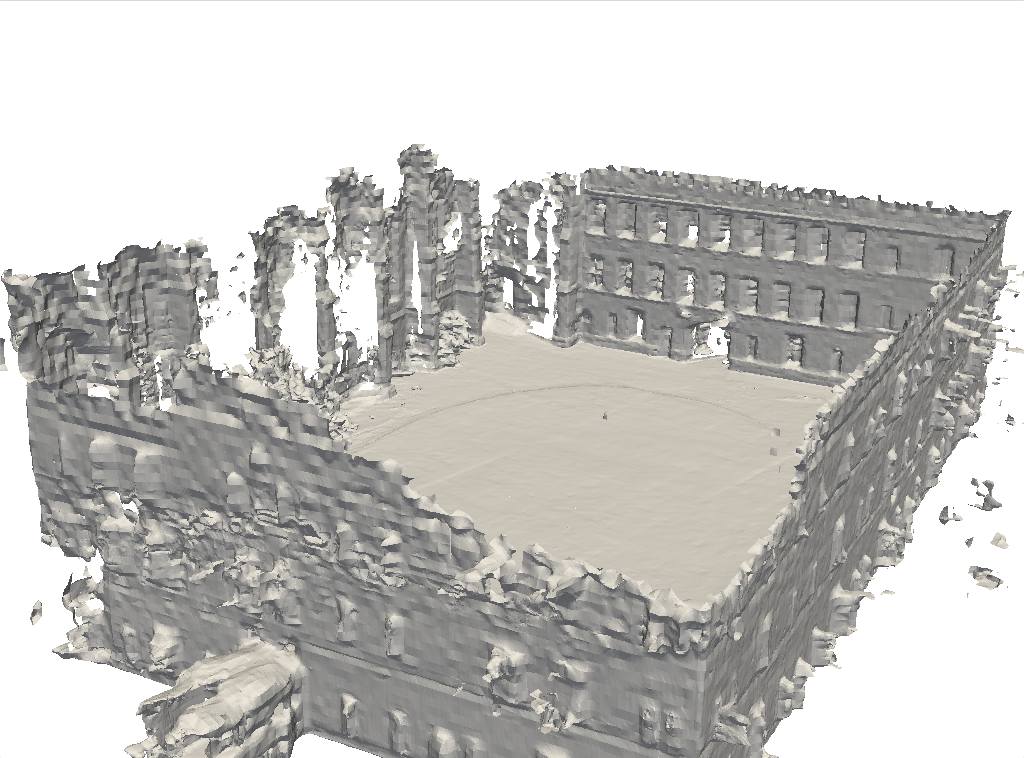
\includegraphics[width=1\linewidth]{figures/ncd_3_bce.png}
\end{minipage}\hfill
\begin{minipage}{0.322\linewidth}
    \centering
    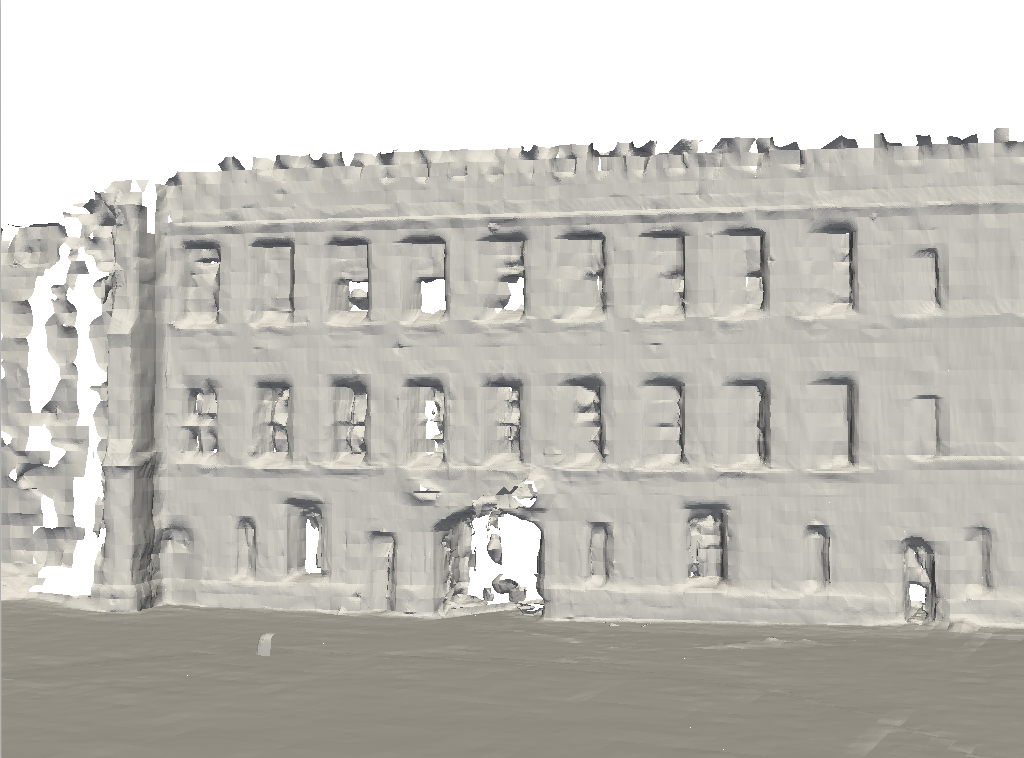
\includegraphics[width=1\linewidth]{figures/ncd_2_bce.png}
\end{minipage}\hfill
\begin{minipage}{0.322\linewidth}
    \centering
    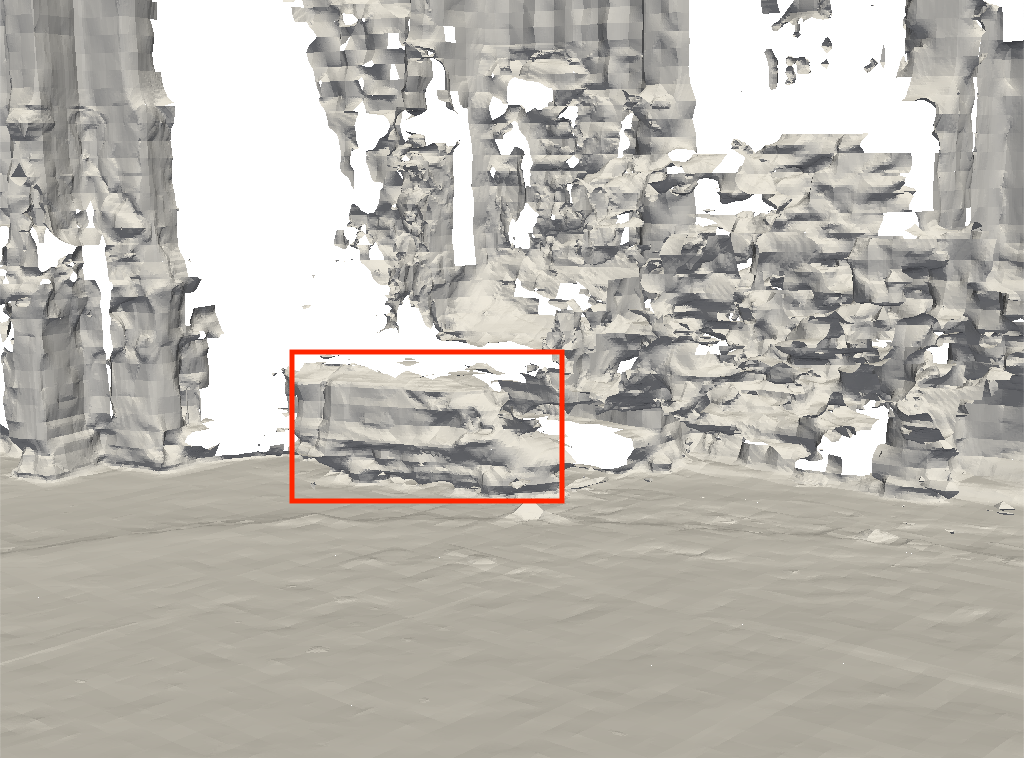
\includegraphics[width=1\linewidth]{figures/ncd_1_bce.png}
\end{minipage}\vfill
(c)
\begin{minipage}{0.322\linewidth}
    \centering
    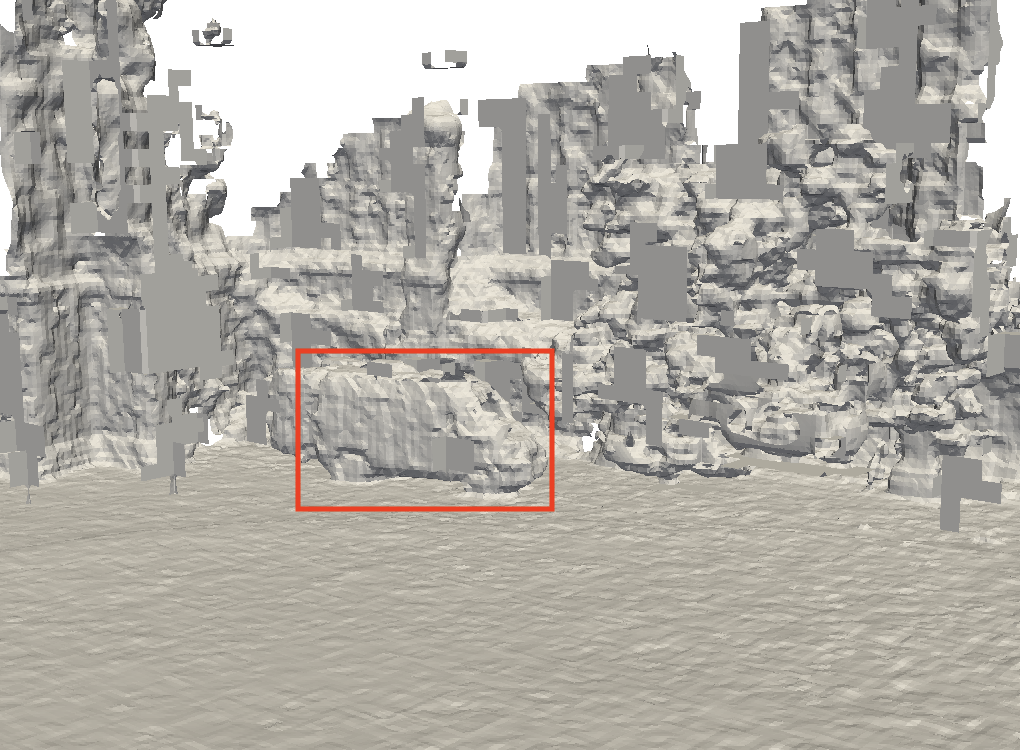
\includegraphics[width=1\linewidth]{figures/ncd_3_shine.png}
    \end{minipage}\hfill
    \begin{minipage}{0.322\linewidth}
    \centering
    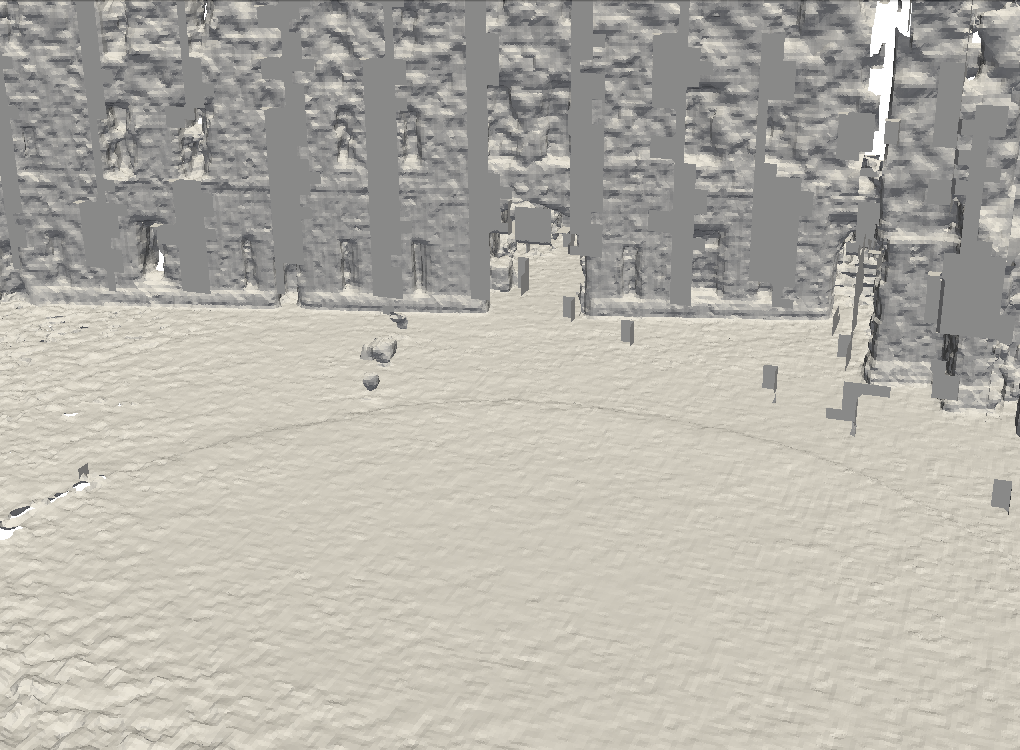
\includegraphics[width=1\linewidth]{figures/ncd_2_shine.png}
    \end{minipage}\hfill
    \begin{minipage}{0.322\linewidth}
        \centering
        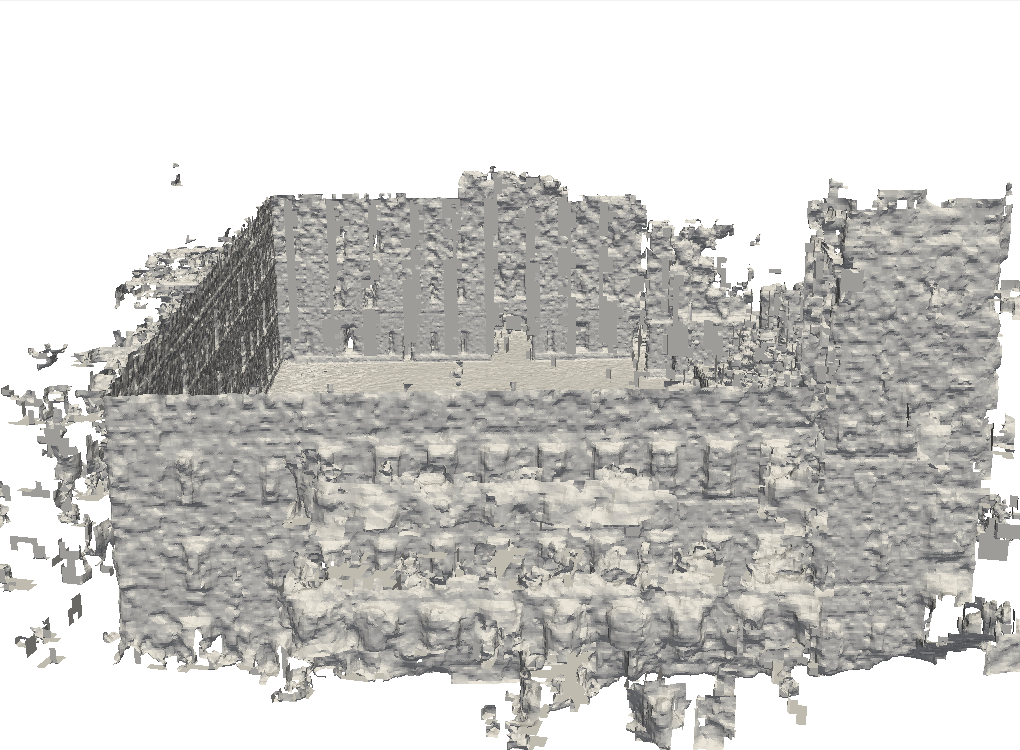
\includegraphics[width=1\linewidth]{figures/ncd_1_shine.png}
        \end{minipage}
    \caption{3种基于神经网络的隐式建图方法在New College数据集上的结果。分别为(a)本文方法, (b)Vox-Fusion与(c)SHINE-Mapping。}\label{ncdresult}
\end{figure}

\begin{table}[htbp]
    \centering
    \caption{定性测量的不同方法在New College数据集上建图的几何精度,将目标地图与重建地图之间对应点重合的阈值$threshold$设置为20cm。}\label{ncdmetric}
    \begin{tabular}[htbp]{llccccc}
        \toprule
        \multicolumn{2}{l}{方法} & $\mathbf{Comp.}$(cm) & $\mathbf{Acc.}(\%)$ & $\mathbf{C-l1}$(cm) &  $\mathbf{Comp. Ratio}$(\%) &$\mathbf{F1-score}$\\
        \midrule
        \multicolumn{2}{l}{Voxblox} & 14.9 & 90.6 &12.1 &87.8&87.9\\
        \multicolumn{2}{l}{VDB Fusion} & 12.0&92.1&9.4&91.3&92.6 \\
        \multicolumn{2}{l}{SHINE-Mapping} & 10.0&93.5&8.4&93.6&93.7 \\
        \multicolumn{2}{l}{Vox-Fusion} & 14.2 & 89.7& 13.6&89.4&89.0\\
        \midrule
        \multicolumn{2}{l}{Ours+bce} &10.3& 93.2 & 7.9 &93.5&91.3\\
        \bottomrule
    \end{tabular}
\end{table}
本文在KITTI数据集上进行了语义建图精度评估实验。如表\ref{kittimetrics}所示,在KITTI数据集的8个序列上,本文对每个关键帧采样1000个点云,使用训练完成的模型与解码器进行推理得到采样点的语义标签,并与SemanticKITTI数据集的语义标签进行比较以计算语义建图精度。结果显示在室外大规模场景下,本文语义建图方法可以达到约90\%的准确率。将预测出的语义标签映射为不同颜色后的效果如图\ref{semresult}所示。这些精确的语义信息可以为无人驾驶系统做出决策提供关键信息。

\begin{table}[htbp]
    \centering
    \caption{本文方法在KITTI数据集上的语义建图精度评估。}\label{kittimetrics}
    \begin{tabular}[htbp]{cccccccccc}
        \toprule
        \multicolumn{2}{l}{指标} & Seq00 & Seq01 & Seq02 &Seq03&Seq04&Seq05&Seq06&Seq07 \\
        \midrule
        \multicolumn{2}{l}{AUC\%} & 91.4 & 92.0 & 89.7 & 90.6 &87.6&88.7&91.2&92.5\\
        \multicolumn{2}{c}{IoU\%} & 83.2& 84.3&79.8&86.2&75.4&77.8&87.3&87.1 \\
        \bottomrule
    \end{tabular}
\end{table}
\begin{figure}[htbp]
	\centering
	\begin{minipage}{0.5\linewidth}
		\centering
		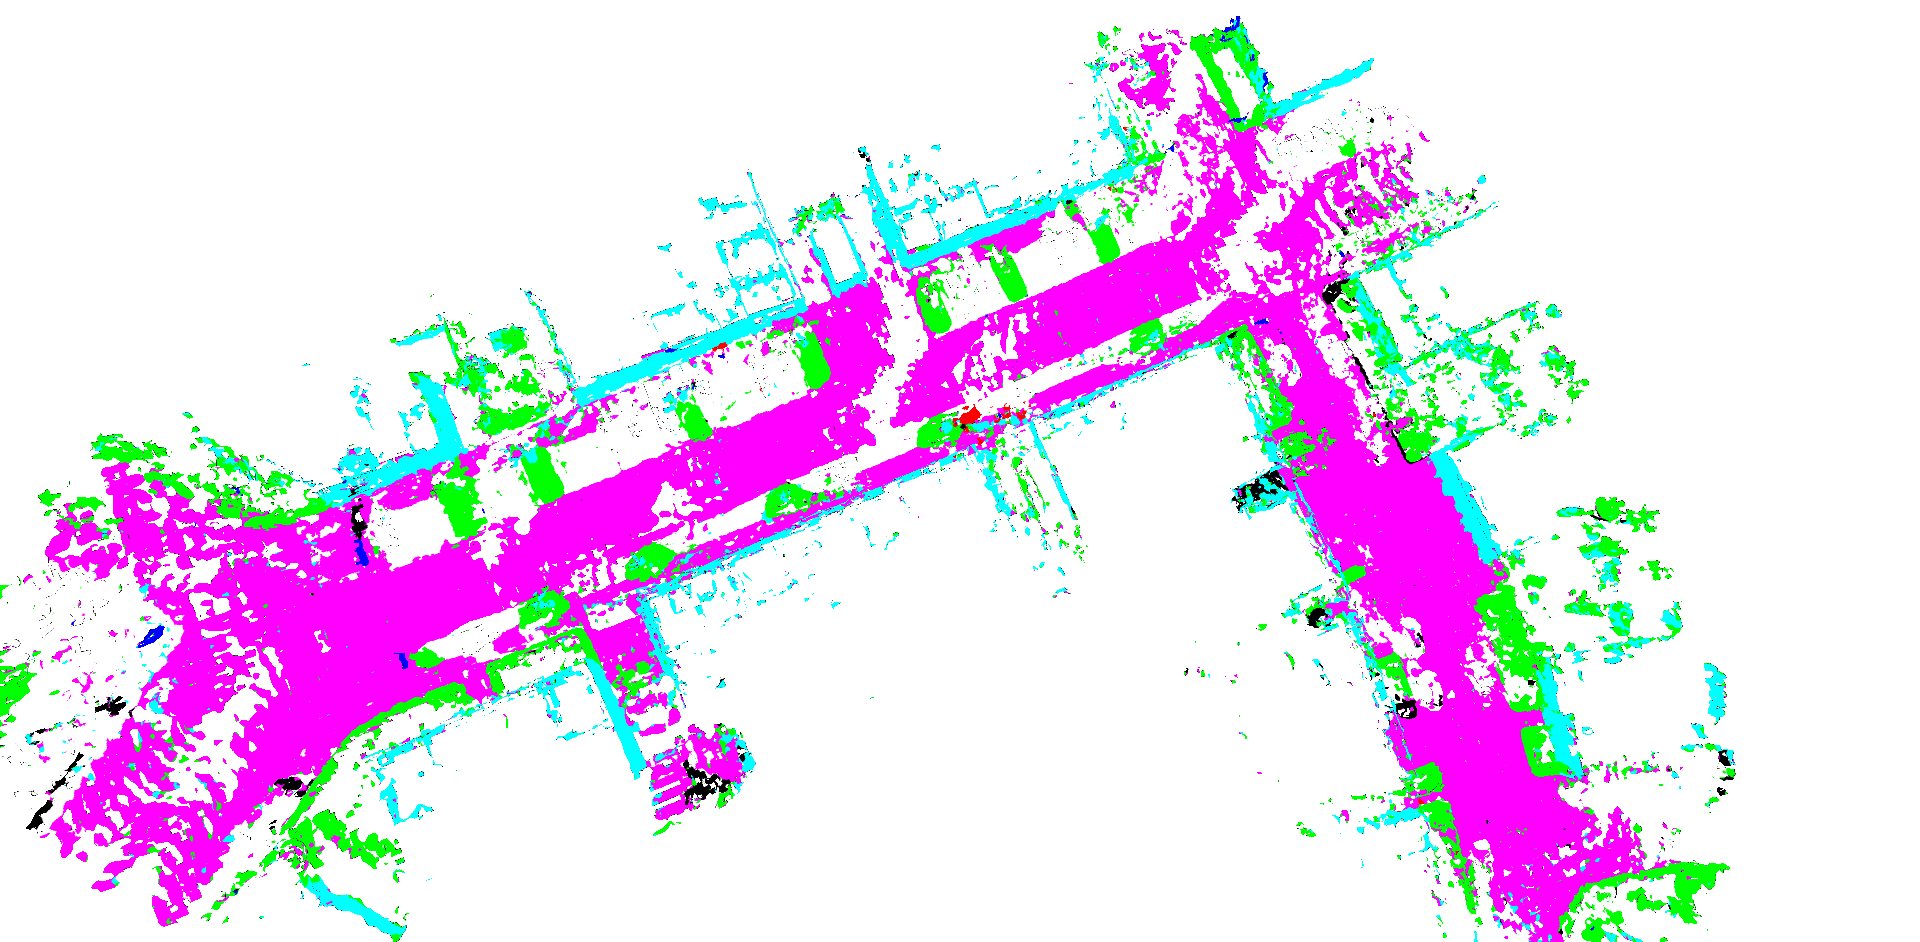
\includegraphics[width=1\linewidth]{figures/sem1.png}
	\end{minipage}\hfill
	\begin{minipage}{0.5\linewidth}
		\centering
		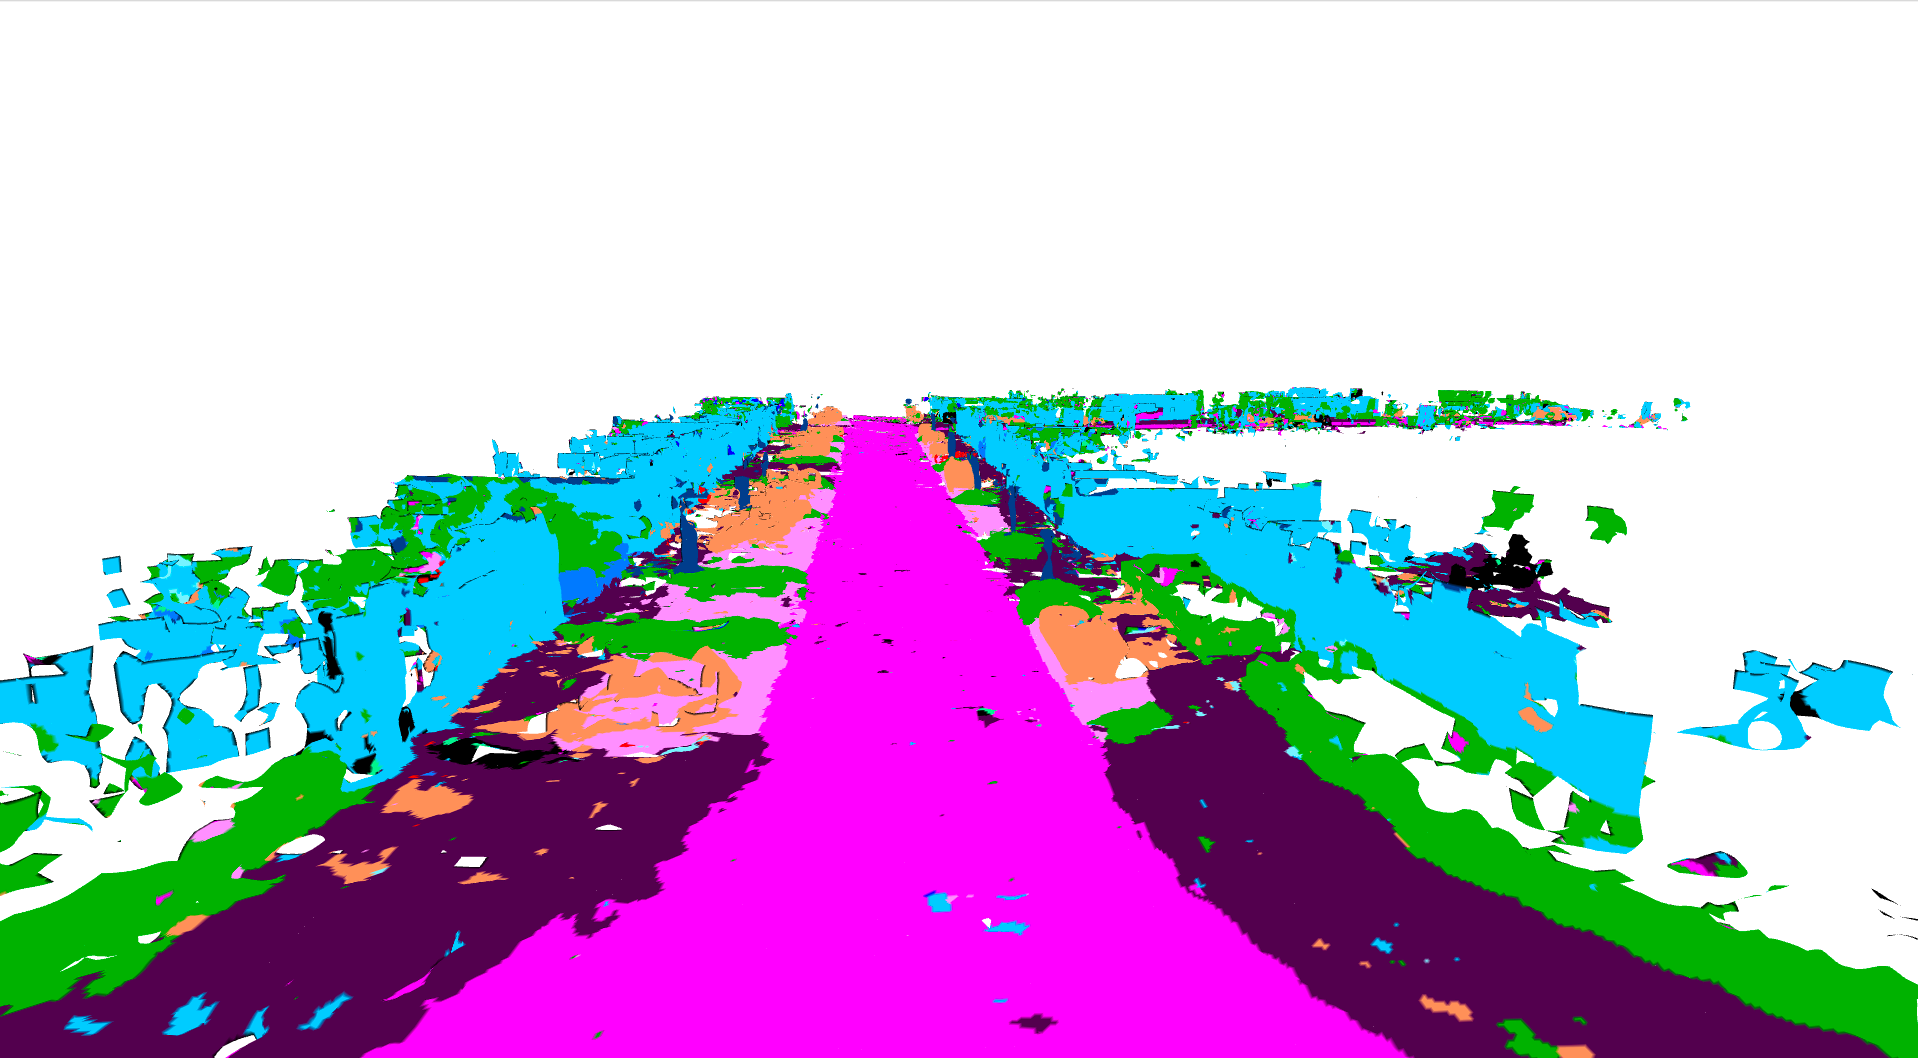
\includegraphics[width=1\linewidth]{figures/sem2.png}
	\end{minipage}
    \caption{在KITTI数据集上进行语义建图后,使用模型预测每一顶点的语义标签并将其映射为不同颜色。其中黑色表示unlabeled顶点,占比极小。本文方法的语义建图可以达到较高的准确率与交并比。}\label{semresult}
\end{figure}

\subsubsection{算法时间与内存占用}
为了加速本文方法,除了使用多线程并行实现增量建图与全局建图外,本文测量了渲染和训练过程中关键步骤的耗时,如体素分配,求交运算和体渲染等步骤,并进行了分析。本文实验在单张Nvidia RTX 3090显卡上进行,结果列于表\ref{times}中。可以看出使用C++实现的体素相关操作运行速度较快,在系统运行中耗时占比远小于其他操作。在采样1024条光线的情况下,本文系统中单次建图迭代需要40-50ms。设置每次建图过程中迭代10-50次,本文系统最快可以达到2Hz的建图速度。
\begin{table}[htbp]
    \centering
    \caption{系统中关键步骤平均耗时。}\label{times}
    \begin{tabular}[htbp]{llc}
        \toprule
        \multicolumn{2}{l}{步骤} & 时间\\
        \midrule
        \multicolumn{2}{l}{增量建图} & 50ms\\
        \multicolumn{2}{l}{全局建图} & 50ms \\
        \midrule
        \multicolumn{2}{l}{体素分配} & 0.1ms \\
        \multicolumn{2}{l}{光线体素求交} & 0.9ms \\
        \multicolumn{2}{l}{体渲染} & 4ms \\
        \multicolumn{2}{l}{参数优化} & 6ms \\
        \bottomrule
    \end{tabular}
\end{table}

相较于同样使用基于体素的八叉树的SHING-Mapping方法,本文方法的内存消耗与其几乎相同。但NICE-SLAM方法使用4个网格地图并需要在系统启动前分配所有地图空间,与之相比本文方法在内存消耗上占据优势。详细结果如图\ref{memory}所示,本文方法可以在显著使用更少内存的同时实现更精细的建模。
\begin{table}[htbp]
    \centering
    \caption{不同方法在Mai City数据集01序列上建图的理论内存消耗。由于NICE-SLAM使用了4个特征网格,每一个特征网格对地图所有区域分配内存,因此内存消耗巨大。本文方法只使用一个特征网格,且只对观察到的地图区域分配体素与特征,使用较小的内存可以达到精细度更高的建图效果。}\label{memory}
    \begin{tabular}[htbp]{llcc}
        \toprule
        \multicolumn{2}{l}{方法} &解码器 & 地图特征\\
        \midrule
        \multicolumn{2}{l}{SHINE-Mapping} & 0.56MB & 7.09MB\\
        \multicolumn{2}{l}{NICE-SLAM} & 0.22MB & 560MB\\
        \midrule
        \multicolumn{2}{l}{Ours} & 1.04MB & 7.09MB\\
        \bottomrule
    \end{tabular}
\end{table}


\newpage
\section{总结与未来工作展望}\label{sec:conclusion}

本节通常用于对论文进行总结和归纳,并提出未来工作的展望和建议。

在总结部分,需要回顾研究内容和方法,对研究结果进行分析和归纳,并阐述研究工作的贡献。同时,也要对研究过程中存在的问题和不足进行反思和总结,为未来的研究提供参考和启示。

在未来工作展望部分,需要具体提出研究计划和建议,为后续研究提供方向和指导。同时,也要对本文提出的方法和技术进行展望,探索其在未来研究中的应用前景和发展方向。此外,还可以指出当前领域中存在的未解决问题,为未来研究提供新的研究思路和方向。

此外,未来工作展望中还可以对本文研究的局限性进行讨论和说明,提出改进和扩展的方向。同时,也要注意将未来工作展望与本文研究内容相互关联,以确保研究的连续性和完整性。

最后,需要强调本文研究的意义和价值,并对读者进行总结和启示,为相关领域的研究提供借鉴和参考。在撰写总结与未来工作展望时,需要遵循逻辑清晰、表达准确、语言简练的原则,使得整篇论文的结论和建议具有可读性和可信度。

\newpage

\addcontentsline{toc}{section}{参考文献}
\bibliography{graduation_thesis}

\newpage
\section*{谢\ 辞}
\addcontentsline{toc}{section}{谢辞}

谢谢支持本项目的所有朋友们。并且希望选用该模板的朋友们都能顺利通过查重与答辩。


\end{document}
